\documentclass{thesis}

\usepackage{rlipsum} % Only needed for Lorem Ipsum dummy text.
\usepackage[T1]{fontenc}
\usepackage{booktabs}

\usepackage{xcolor}

\thesisTitle{Abstraction Discovery in Shape Programs}
\thesisType{Master Thesis}
\thesisAuthor{Amogh Warkhandkar}
\thesisStudentID{442481}
\thesisMonth{February 2026}
\thesisAdvisor{Leonard Schramm}
\thesisPrimaryReviewer{Prof. Dr. Leif Kobbelt}
\thesisSecondaryReviewer{Dr. Isaak Lim}

\begin{document}
\makeFrontMatter

\chapter*{}
\begin{center}
    \textbf{Abstract}\\
\end{center}

A central challenge in neurosymbolic graphics is the automated discovery of programmatic abstractions from hierarchical 3D shape representations. While procedural models provide structural clarity, real-world objects often exhibit complex relationships that rigid symbolic templates cannot capture. Traditional approaches rely on a greedy parametric search over a fixed combination of variables, creating a ``symbolic bottleneck'' where non-linear dependencies remain uncompressed. This thesis introduces a neurosymbolic framework that replaces discrete symbolic matching with the neural modeling of parametric data extracted from a functional DSL. By utilizing parameter clustering and intrinsic dimensionality estimation techniques, the framework identifies the intrinsic degrees of freedom within the data and models them using neural networks like Autoencoders to learn non-linear dependencies between parameters for high-fidelity reconstruction, and Variational Autoencoders for increased latent interpretability and editability. When integrated into an E-graph for structural refactoring, this approach successfully resolves complex parametric variations that symbolic solvers might miss. Evaluated on diverse 3D shape categories, our framework demonstrates the power of combining neural flexibility with symbolic structure to achieve improved program compression as measured by the minimum description length principle.

\mainmatter

%%%%%%%%%%%%%%%%%%%%%
% INTRODUCTION
%%%%%%%%%%%%%%%%%%%%%

\chapter{Introduction}\label{ch:introduction}

Procedural modeling is a powerful method for representing 3D geometry through compact and editable algorithmic descriptions \cite{Ritchie2023}. By encoding shapes as executable programs, these models allow for high-level geometric changes and consistent variations across large datasets. Recent advancements in visual program induction, such as the ShapeCoder framework \cite{ShapeCoder}, have established effective workflows for discovering these programs from unstructured sets of primitives. ShapeCoder uses an iterative process to discover programs, utilizing a Transformer-based recognition network \cite{Vaswani2017} to infer code and E-graphs \cite{Willsey2021} to refactor them into compressed forms. However, while these methods are effective in identifying structural logic, a major problem remains in how parameters are handled, specifically the complex relationships between attributes like position, scale, and rotation.

Currently, parametric discovery is typically treated as a symbolic search problem \cite{ShapeMOD}. This process attempts to match part variations against a fixed library of symbolic templates, which are mostly limited to simple equations. This strategy has two main limitations when used for complex datasets like PartNet \cite{Yu_2019_CVPR, Mo_2019_CVPR}. First, symbolic search is often too rigid to capture the complex, non-linear relationships found in varied object designs. Second, as the number of parameters increases, the search becomes too slow, forcing the use of simplifications that often miss important patterns. When a relationship does not match a predefined formula, the system is forced to treat every variable as independent, which leads to uncompressed programs and fails to reach the optimal Minimum Description Length (MDL) \cite{Rissanen1978}.

This thesis proposes a move from rigid symbolic matching toward neural abstractions. This approach is based on the idea that high-dimensional data often follows a simpler, lower-dimensional structure, known as the Manifold Hypothesis. Our system uses the E-graph as the core tool for structural discovery but replaces traditional symbolic matching with learned data distributions. Instead of searching for a perfect equation in a limited library, we model the parameter space as a continuous distribution. By using Local Intrinsic Dimensionality (LID) \cite{IntrinsicDim, faccotwonn} to determine how much the data can be simplified, the system identifies the underlying variables directly from the data. These relationships are then modeled using neural networks like Autoencoders (AEs) and Variational Autoencoders (VAEs). This approach allows us to discover abstractions that are structurally consistent but flexible enough to capture complex geometric relationships.

To address these limitations, this thesis introduces a neurosymbolic framework with two main contributions:

\begin{itemize}
    \item \textbf{LID-Guided Parameter Analysis:} A method for finding the underlying variables within part parameters using Local Intrinsic Dimensionality (LID). This provides a solid foundation for grouping parameters using \textbf{HDBSCAN} and ensures the neural networks are trained on stable and meaningful patterns.
    \item \textbf{Neural Parametric Abstractions:} A set of neural compression models that replace fixed equations with stable latent representations. By utilizing Lipschitz-constrained VAEs, these ``neural macros'' achieve better compression while ensuring the model remains stable for smooth geometric editing.
\end{itemize}

These components are combined in a pipeline that uses the \texttt{egglog} engine to refactor the program structure. By using a weighted cost model, the system finds the best place for neural abstractions to minimize the total program length across the dataset.

We evaluate our framework on the PartNet dataset, showing that neural abstractions can handle complex design variations where traditional symbolic methods fail. Our results show that by moving from fixed templates to learned distributions, we significantly reduce the program length while maintaining high reconstruction accuracy, especially on high-precision datasets. 

The thesis is structured as follows: Chapter \ref{ch:background} provides the background on procedural modeling, E-graphs, and intrinsic dimensionality. Chapter \ref{ch:related_work} reviews existing work in program induction and the ShapeCoder framework. Chapter \ref{ch:methods} presents our main technical contribution, detailing how we extract structure and train the neural models. Chapter \ref{ch:evaluation} evaluates our approach with both qualitative and quantitative comparisons. Finally, Chapter \ref{ch:conclusion} summarizes our findings and discusses future work.

%%%%%%%%%%%%%%%%%%%%%
% BACKGROUND
%%%%%%%%%%%%%%%%%%%%%

\chapter{Background}\label{ch:background}

%%%%%%%%%%%%%%%%%%%%%
% BACKGROUND >>> Procedural Modeling
%%%%%%%%%%%%%%%%%%%%%

\section{Procedural Modeling}\label{back_procedural}

\begin{figure}[htbp]
    \centering
    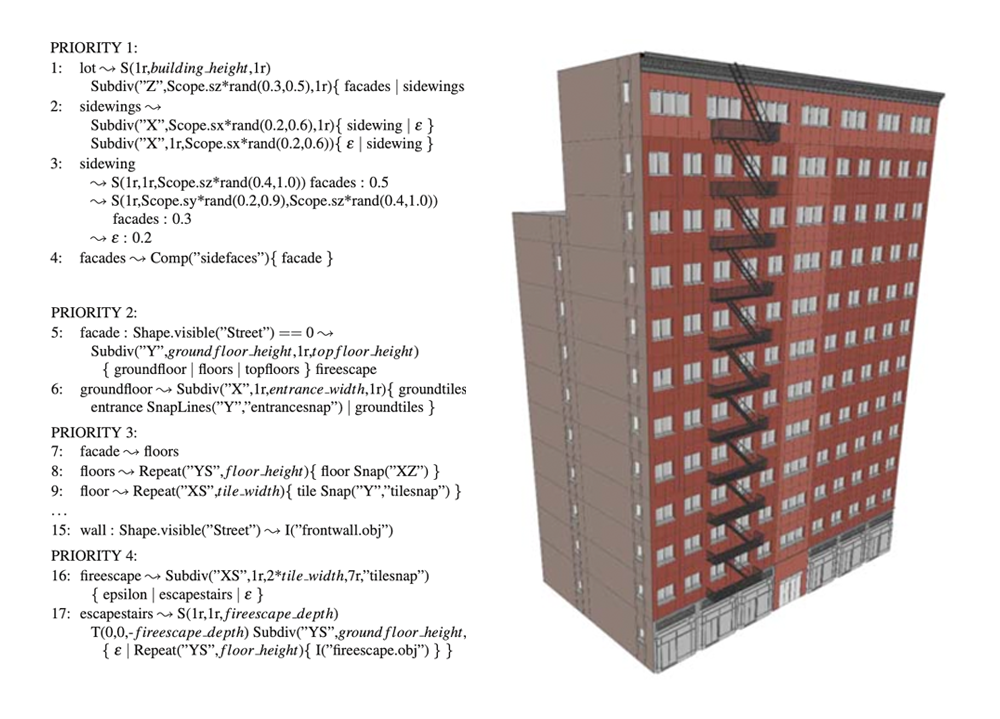
\includegraphics[width=\textwidth]{figures/Muller2006Procedural.png}
    \caption{Example of grammar based procedural modeling. Production rules (left) are used to iteratively transform a base primitive into a detailed architectural model (right) by defining spatial relationships and repetitive patterns across different scales of the facade. Original Figure from \cite{Muller2006}}
    \label{fig:Muller2006Procedural}
\end{figure}

Procedural modeling has remarkably changed the way geometric models are generated, allowing the automated creation of detailed structures ranging from individual architectural components to large-scale urban environments \cite{Muller2007, Demir2014}. At its core, this approach uses Domain-Specific Languages (DSLs) to convert high-level algorithmic rules into concrete geometric representations \cite{Muller2006}. By defining shapes through symbolic logic rather than vertex-level geometry, these systems provide a powerful toolkit for generating high-resolution models that maintain structural consistency across varied scales and configurations.

\subsection{Shape Programs}

At the heart of procedural modeling is the concept of a \textit{shape program}. A shape program is a symbolic, executable representation of a 3D object, typically expressed in a functional DSL. For example, a shape can be defined as the result of a composition of functions that create, combine, or modify geometry. 

\begin{figure}[htb]
    \centering
    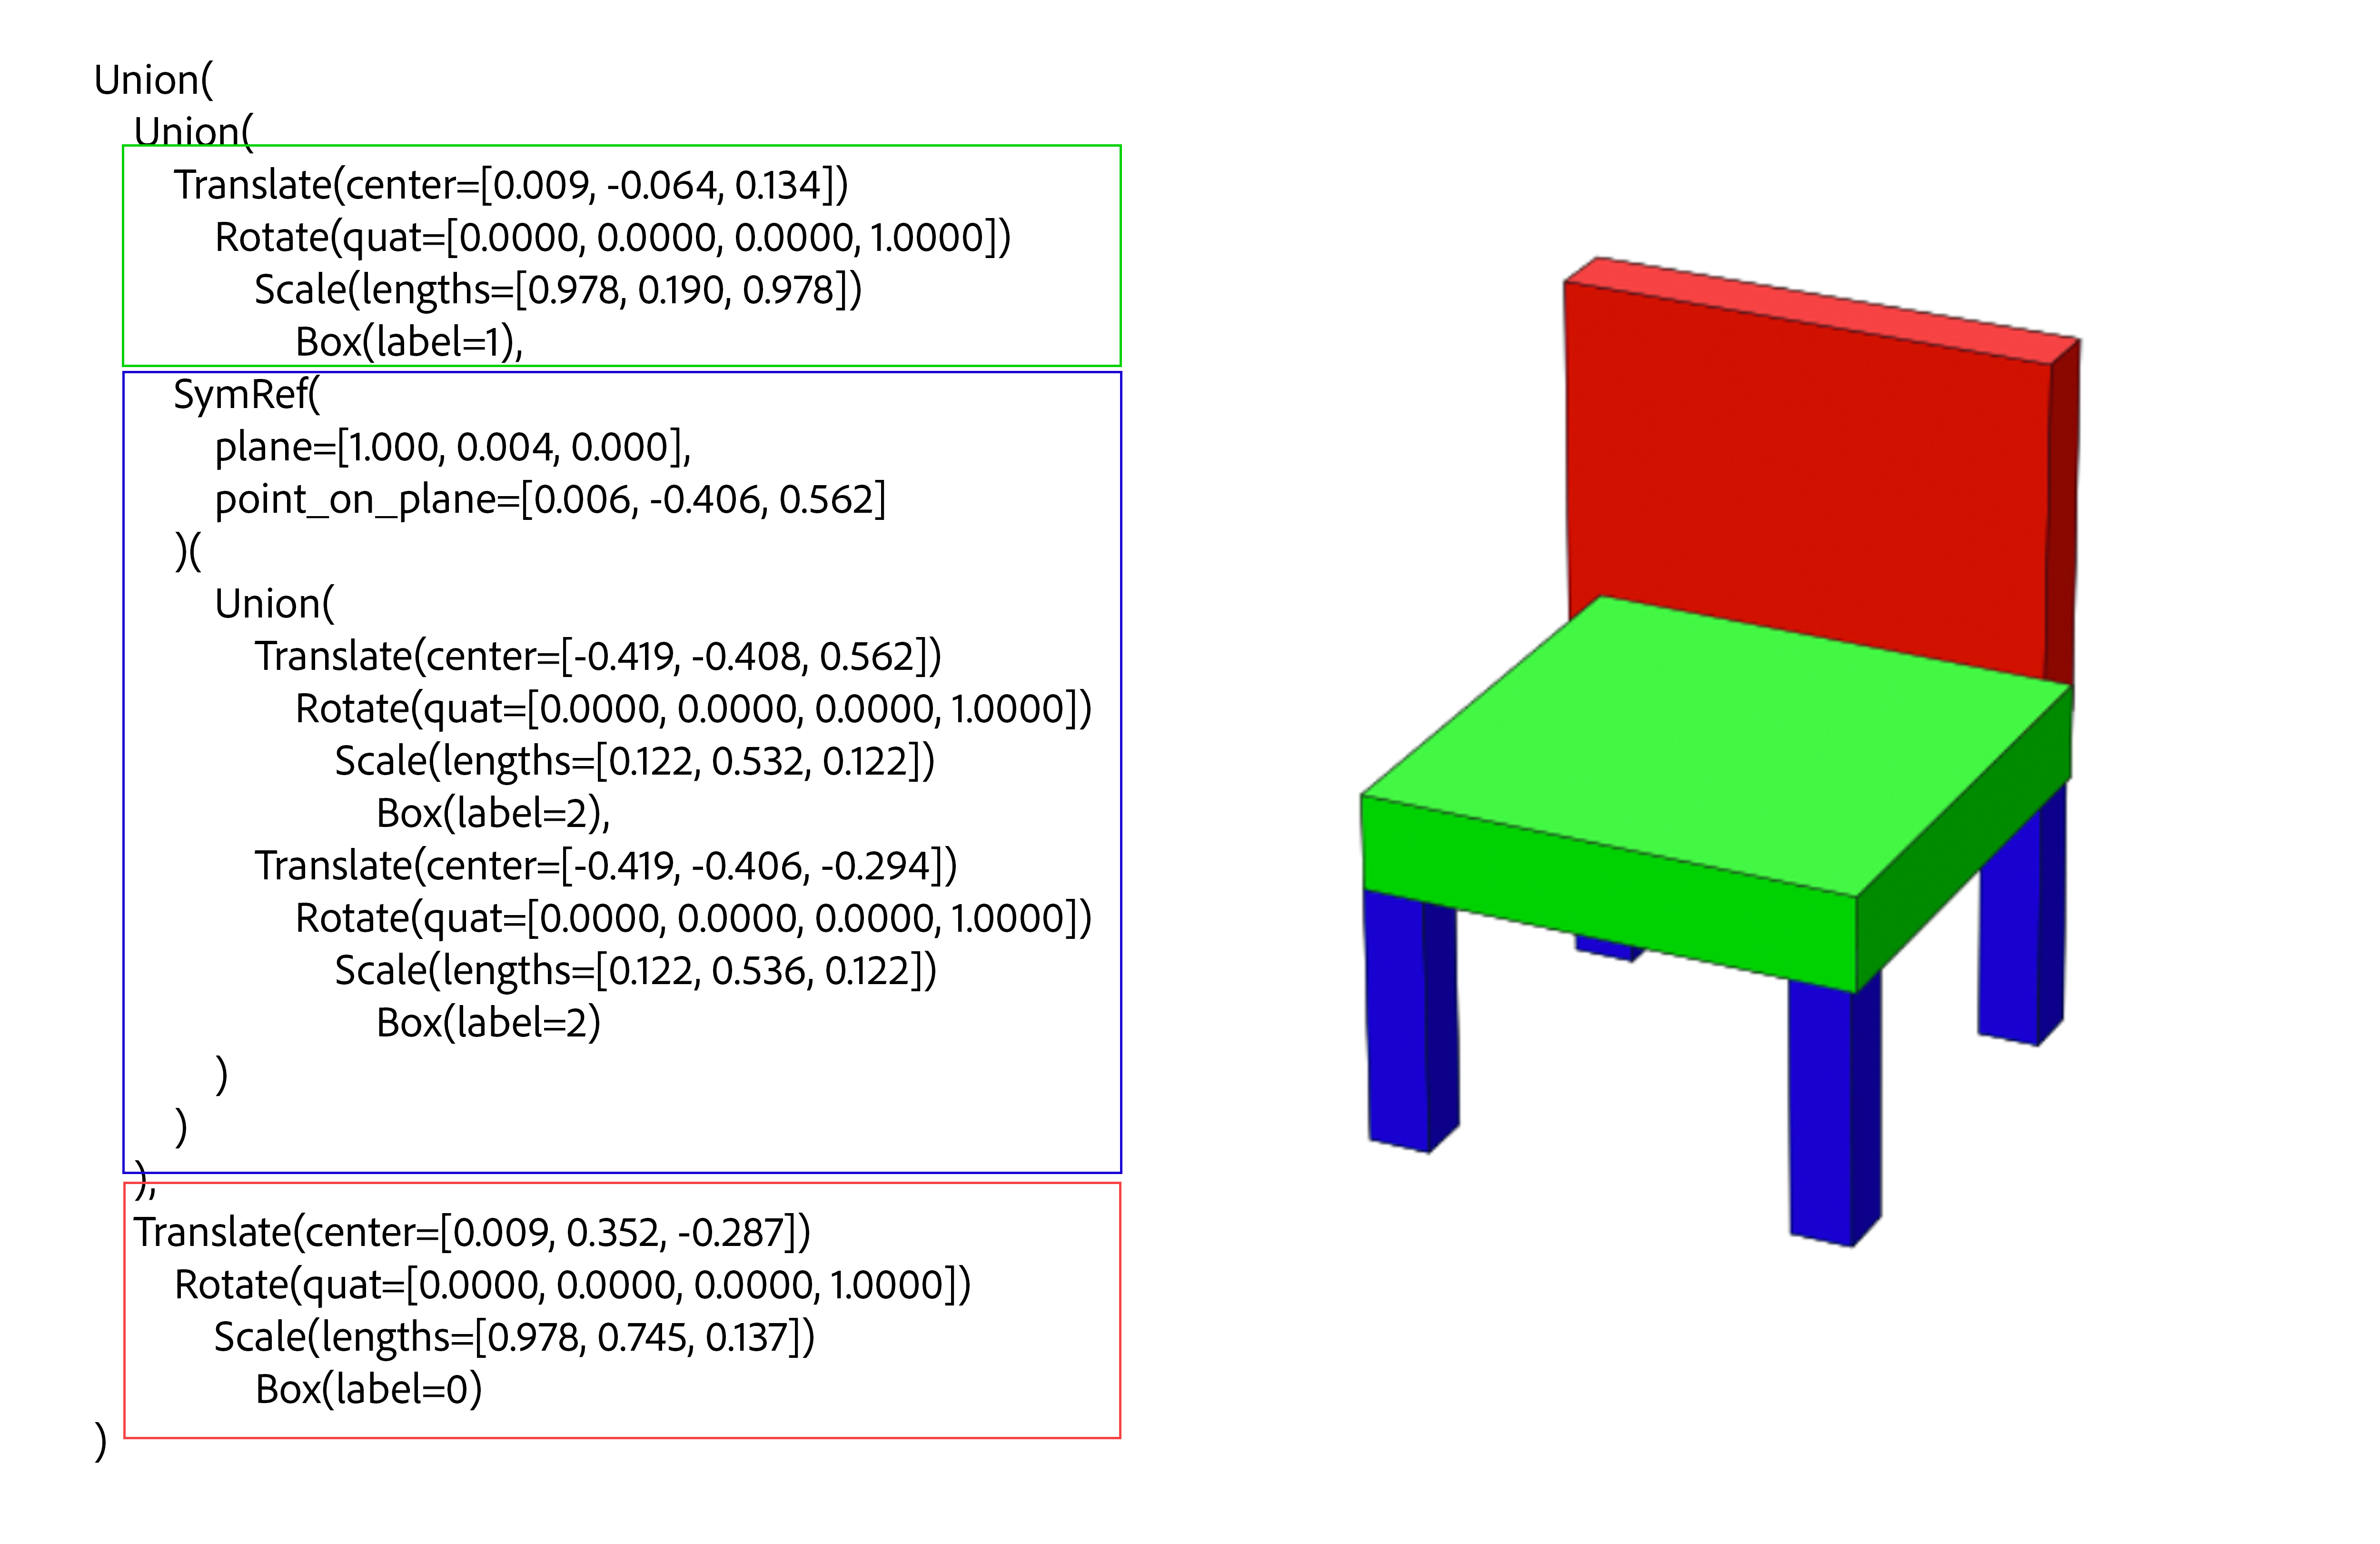
\includegraphics[width=0.8\textwidth]{figures/dslexample.png}
    \caption{Example of a shape program from the PartNet dataset. The code is highlighted to show the relation between specific code blocks and the resulting parts of the 3D model: the backrest (red), seat (green), and leg assembly (blue).}
    \label{fig:PartnetSymhChair}
\end{figure}

These functions are generally parameterized by two types of variables:
\begin{itemize}
    \item \textbf{Discrete Parameters:} These define categorical or structural choices, such as semantic labels (e.g., \texttt{Box(label=2)} for a leg) or fixed rotation axes (e.g., \texttt{AX}, \texttt{AY}, \texttt{AZ}).
    \item \textbf{Continuous Parameters:} These define the geometric attributes of a part, for example its position (translation), orientation (rotation/quaternion), and dimensions (scale).
\end{itemize}

Before we understand the automated discovery of these programs, it is essential to distinguish between the two primary design principles of DSL structure: imperative and declarative.

\begin{figure}[htb]
    \centering
    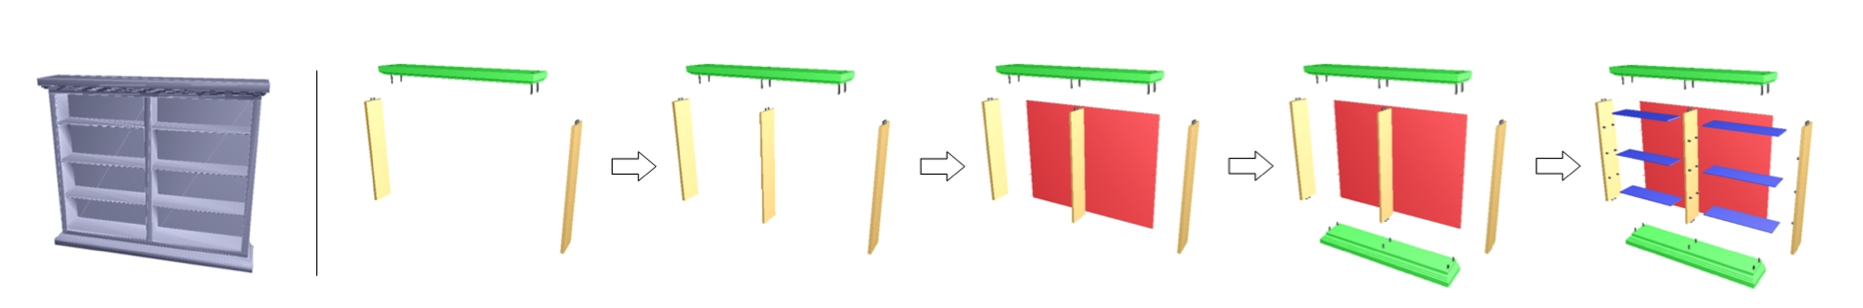
\includegraphics[width=\textwidth]{figures/Lau2011PartConnections.png}
    \caption{Example of a sequential construction process of a Bookshelf in imperative procedural modeling. The workflow shows the breakdown of a 3D model into an ordered series of parts and connectors, showing how imperative systems define geometry through a path-dependent sequence of steps. Original Figure from \cite{Lau2011}}
    \label{fig:Lau2011PartConnections}
\end{figure}

Imperative frameworks define geometry through a sequence of modeling commands, where the final state is reached via steps of discrete transformations. A classic example is \textit{L-systems}, which use production rules to simulate organic growth in plants or street networks based on local parameters \cite{Parish2001, Stava2014}. While effective for modeling stochastic growth, imperative representations are inherently order-dependent, which complicates structural analysis. The final geometry emerges from a path-dependent process, making it challenging to reconstruct a static, hierarchical graph. Furthermore, these models are often non-differentiable and highly non-linear, creating major challenges for optimization using standard gradient-based deep learning methods. As illustrated in Figure \ref{fig:Lau2011PartConnections}, the sequential nature of these frameworks prioritizes the construction path over global structural relationships.

\begin{figure}[htb]
    \centering
    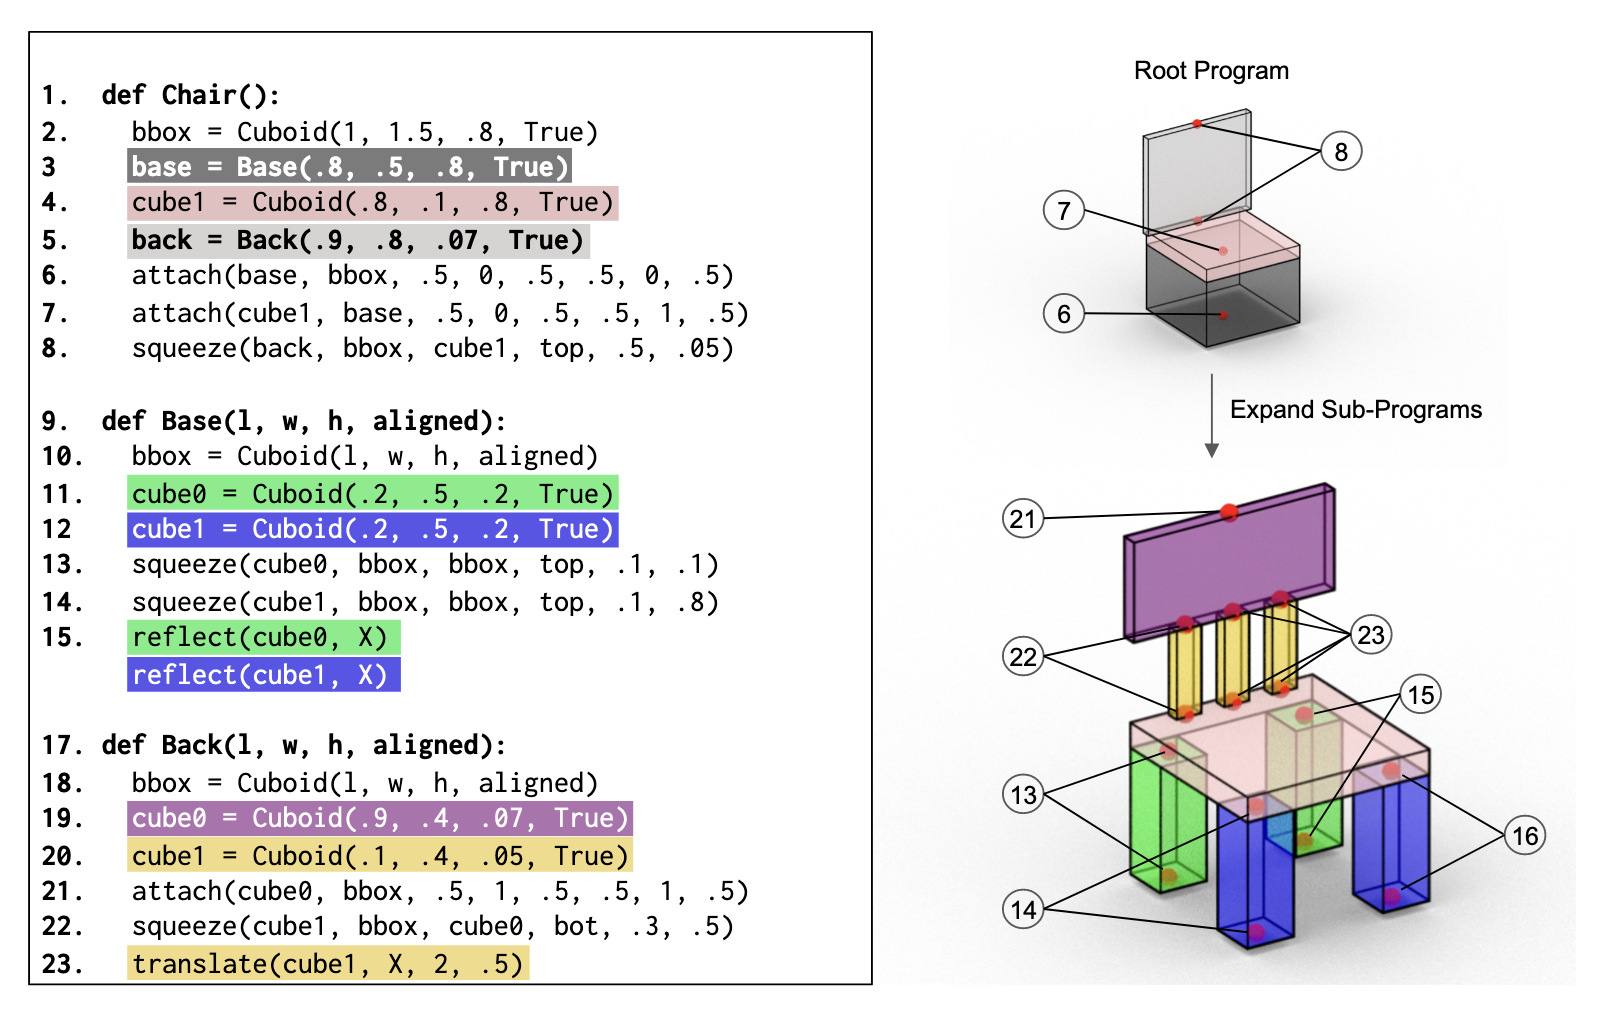
\includegraphics[width=\textwidth]{figures/ShapeAssemblyExample.png}
    \caption{Overview of the ShapeAssembly's DSL. The hierarchical program (left) utilizes geometric primitives and attachment commands such as cuboid, attach, and squeeze to define the structural relationships of a 3D shape. The execution flow (right) illustrates the expansion from a root program into a fully developed assembly. Original Figure from \cite{ShapeAssembly}}
    \label{fig:ShapeAssemblyExample}
\end{figure}

In contrast, declarative representations describe the state of a shape rather than the process of its construction. This concept prioritizes the spatial and semantic relationships between constituent parts, as shown by the \textit{ShapeAssembly} DSL \cite{ShapeAssembly} (Figure \ref{fig:ShapeAssemblyExample}). Since declarative models define a static relationship graph rather than a sequential path, they provide a more stable and interpretable foundation for program induction. By parameterizing these functions with continuous variables, procedural rules can be mapped into the high-dimensional latent spaces of neural networks, allowing for effective neurosymbolic integration.

Using these programmatic building blocks, we can perform \textit{abstraction discovery}. In this context, finding an abstraction means identifying structural patterns that repeat across different shapes and turning them into reusable components, often called macros. For example, instead of describing every coordinate for four identical chair legs separately, we can define one ``leg'' function and reuse it with different parameters. This process simplifies the programs by replacing many low-level details with high-level, semantic concepts.

However, because there are many different ways to abstract a given shape, we need a formal way to decide which representation is the most efficient that balances the simplicity of a program against its accuracy.

\section{Minimum Description Length}\label{back_neurosymbolic}

Ritchie et al. \cite{Ritchie2023} mention that while procedural models provide increased interpretability and ease of modification, they are quite difficult to author manually. And while neural networks are efficient at learning from data, they can produce geometric artifacts that distort the shape program. To combine these strengths, we need a formal way to identify which programmatic components simplify the representation without sacrificing its geometric fidelity.

We use the Minimum Description Length (MDL) principle \cite{Rissanen1978} to decide which components are worth adding to our library. The core concept is that the most effective model is the one that provides the shortest overall description of the dataset. This requires finding an optimal balance between the discrete structure of the program and its continuous parameters. By favoring the simplest explanation that still explain the data, MDL can be thought of as a mathematical version of Occam's Razor.

Exploration-Compression algorithm \cite{Dechter2013} and the DreamCoder framework \cite{DreamCoder} have framed abstraction discovery as a library learning problem. By identifying common patterns across different shapes, we can save them as reusable macros. This makes learning easier over time. For example, once the system learns a ``chair leg'', it can reuse that part instead of describing it from scratch every time. This simplifies the programs and allows the system to focus on discovering even more complex patterns.

We evaluate these benefits using an objective function $F(L, P)$ that weighs structural savings against geometric accuracy:

\begin{equation}\label{eq:mdl_cost}
    F(L, P) = \underbrace{\mathcal{L}(L, P)}_{\text{Complexity Cost}} + \underbrace{\mathcal{L}(D | L, P)}_{\text{Residual Cost}}
\end{equation}

In this objective function, $L$ represents the library of abstractions, $P$ is the set of programs representing the shapes, and $D$ true geometric data. The term $\mathcal{L}$ denotes the description length (or cost) of those components.  Specifically:
\begin{itemize}
    \item The Complexity Cost $\mathcal{L}(L, P)$ measures the length of the code needed to define the shared library and the resulting programs.
    \item The Residual Cost $\mathcal{L}(D | L, P)$ tracks the geometric difference between the program's output and the original data $D$. 
\end{itemize}

Finding the optimal configuration of abstractions that minimizes this objective requires a scalable method for program refactoring. To address this, E-graphs are used to represent the space of possible programs, and equality saturation is used to explore the space of possible programs in a non-destructive way, avoiding the problems of greedy, sequential optimization.

\section{E-graphs and Equality Saturation}\label{back_egraphs}

\begin{figure}[htbp]
    \centering
    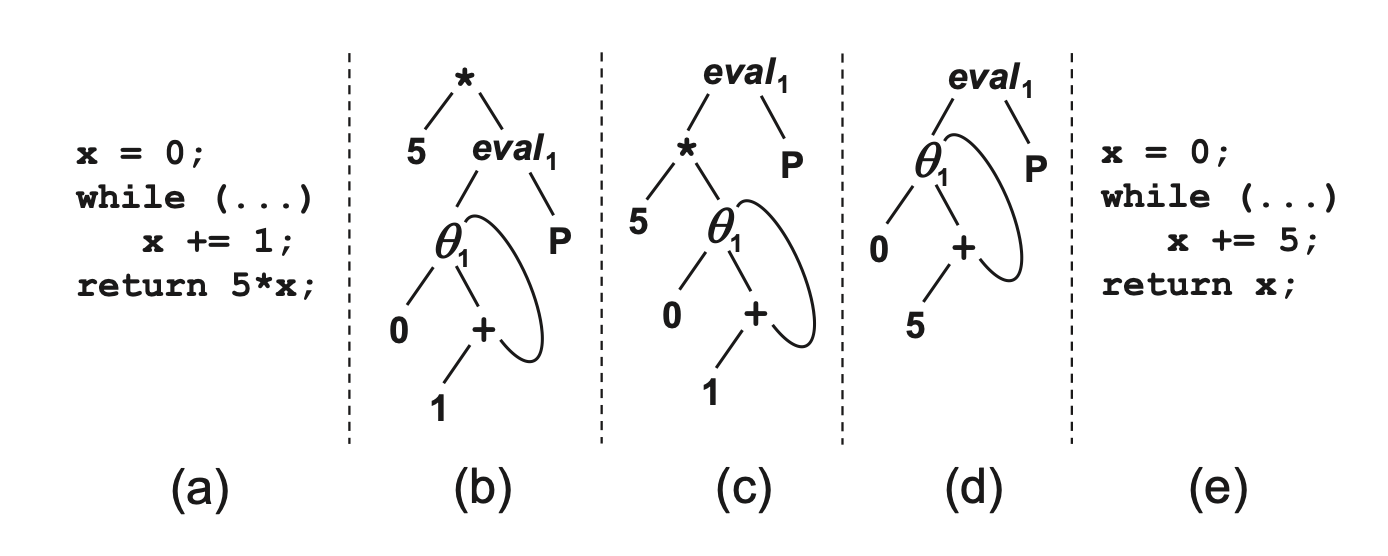
\includegraphics[width=\textwidth]{figures/Tate2009eqsat.png}
    \caption{Iterative loop optimization via algebraic identities: (a) initial source, (b) original Program Expression Graph, (c–d) saturation including induction-variable strength reduction, and (e) the optimized output. This illustrates how equality saturation optimizes complex control flow non-destructively, overcoming the phase-ordering problem by allowing a global heuristic to select mathematically superior results. Original Figure from \cite{Tate2009}.}
    \label{fig:Tate2009eqsat}
\end{figure}

E-graphs have emerged as a robust solution for managing program transformations, specifically addressing the phase ordering problem in compiler design \cite{wiki_egraph, Tate2009, Willsey2021}. Traditional optimization pipelines are often destructive, meaning that applying a rewrite rule replaces the original expression with a transformed version. This sequential nature can be problematic, as a locally beneficial choice might obscure a more optimal global transformation later in the process, effectively trapping the search in a suboptimal state \cite{Joshi2002}. In contrast, E-graphs provide a non-destructive alternative by maintaining a unified representation of all equivalent expressions discovered during the search; this process of non-destructive algebraic exploration is illustrated in Figure~\ref{fig:Tate2009eqsat}.

The power of the E-graph lies in its ability to store an expansive version space within a compact memory footprint through aggressive structural sharing \cite{Nelson1980, Willsey2021}. Formally, the structure defines an equivalence relation over terms in a domain-specific language. It is built from two fundamental units: \textbf{e-nodes} and \textbf{e-classes}. An e-node represents a functional application where the children are pointers to e-classes rather than direct references to other nodes. An e-class acts as a persistent container for all e-nodes that have been proven semantically identical. By decoupling the operator from its children, the E-graph can represent an exponential number of equivalent programs while avoiding the memory explosion typical of standard forest structures.

To ensure the internal consistency of this representation, the E-graph relies on two core invariants: \textbf{congruence} and \textbf{hashconsing}. The congruence invariant dictates that the equivalence relation must be closed under function application; if two sets of arguments are proven equivalent, their respective function calls must also reside in the same e-class. Simultaneously, the hashconsing invariant ensures that every unique e-node is mapped to a singular e-class identifier, preventing redundant storage of identical terms. These properties are typically implemented through a combination of a Union-Find data structure for class management and a hash map for efficient node lookups \cite{Willsey2021}.

The population of an E-graph is performed through a process known as \textbf{equality saturation}. During this phase, the system repeatedly identifies patterns in the graph via e-matching and incorporates equivalent representations based on a library of rewrite rules. Unlike traditional methods, this process only adds information without discarding existing versions. The search continues until the graph reaches a fixed-point or saturation where no further identities can be derived. This approach allows the system to explore the full space of equivalent programs simultaneously, discovering complex refactorings in a single pass without the need for manual ordering or backtracking.

Once the search is completed, an extraction procedure is used to identify the most efficient program from the saturated graph based on a cost model, such as the MDL principle \cite{Tate2009, Willsey2021}. While finding the absolute lowest-cost program is generally NP-hard, it still remains computationally feasible for many practical induction tasks. However, the search complexity must be carefully managed, as the exponential growth of the version space can lead to performance bottlenecks if not constrained by appropriate cost heuristics. Recent advancements like the \texttt{egg} library \cite{Willsey2021} have further optimized this workflow through rebuilding, a technique that improves performance by deferring invariant maintenance to the boundaries of rewrite cycles.

\section{Intrinsic Dimensionality}\label{back_lid}

The estimation of intrinsic dimensionality (ID) is a critical component for effectively modeling high-dimensional shape parameters. Achieving optimal compression requires distinguishing between the observed \textit{extrinsic} parameters and the underlying \textit{intrinsic} degrees of freedom \cite{bernstein2020}.

\subsection{Intrinsic vs. Extrinsic Dimensionality}

\begin{figure}[htbp]
    \centering
    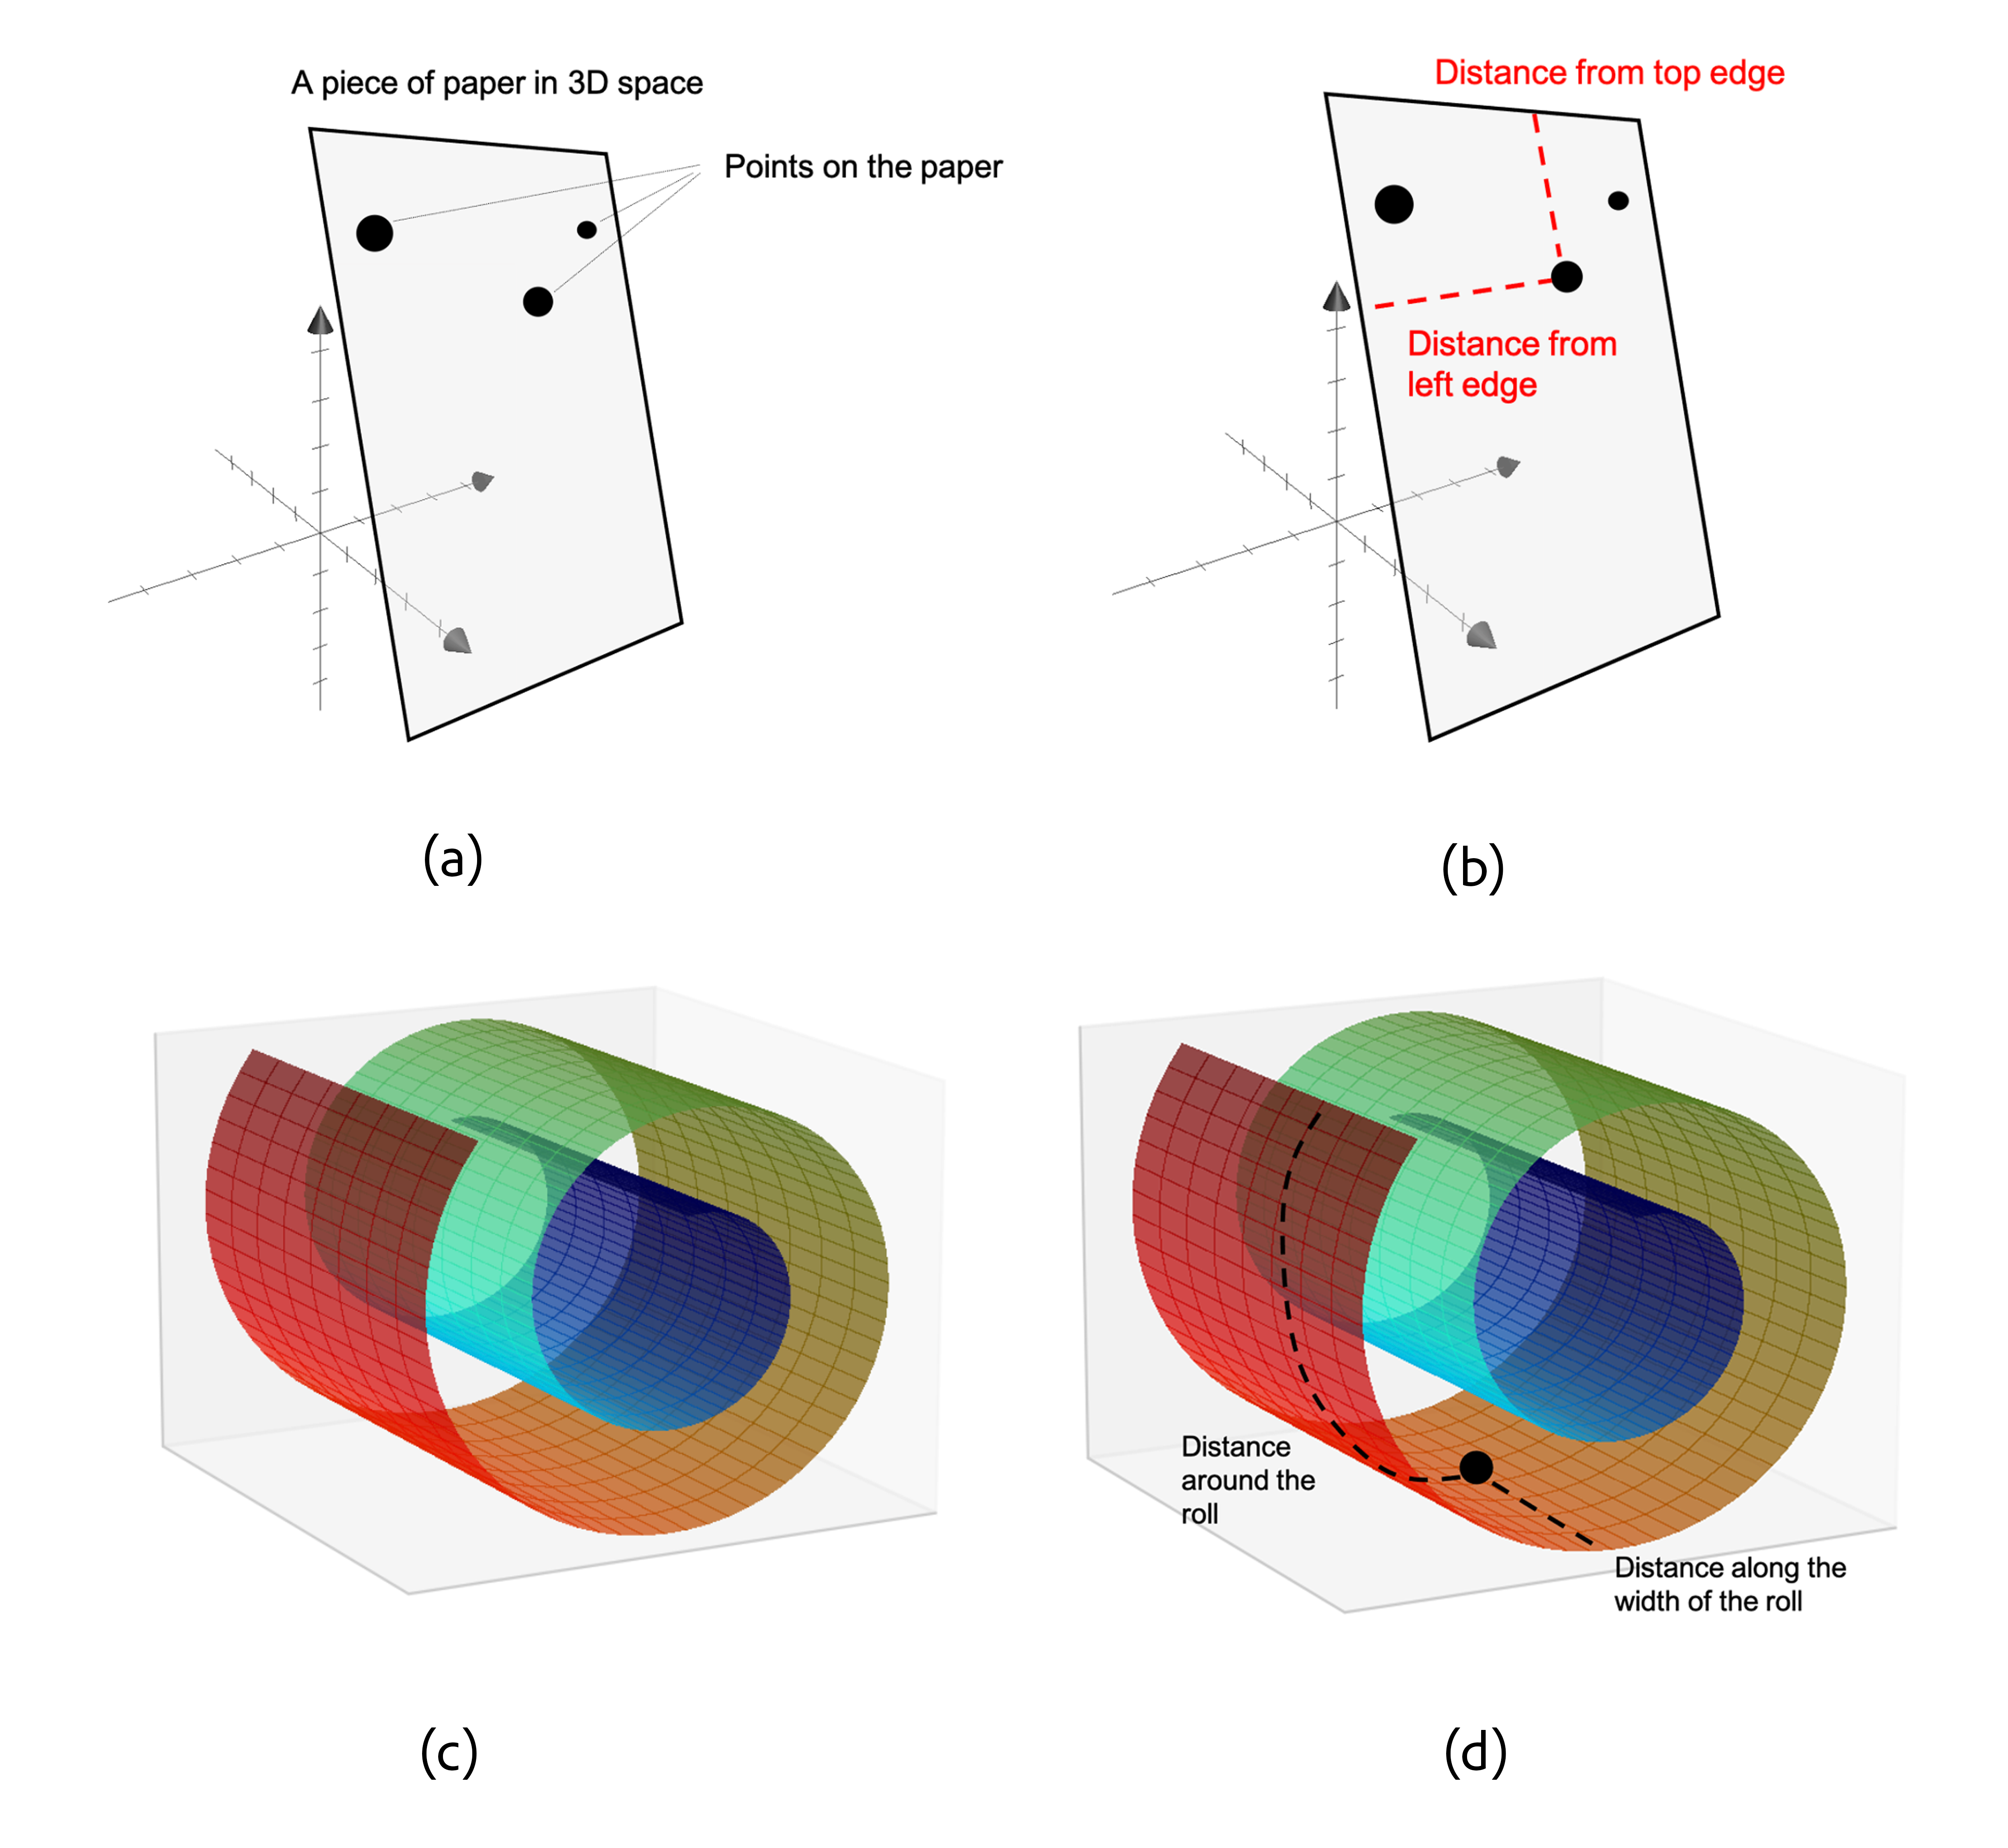
\includegraphics[width=0.95\textwidth]{figures/backlid.png}
    \caption{Geometric intuition of intrinsic versus extrinsic dimensionality. (a-b) A flat sheet of paper embedded in 3D: although points are defined by global $(x, y, z)$ coordinates, they occupy an intrinsically 2D space as they can be uniquely parameterized by two local surface variables. (c-d) A non-linear Swiss roll manifold: despite the complex embedding in 3D, the data is intrinsically 2D, as any point is fully described by its width and its distance along the rolled surface. Original Figures from \cite{bernstein2020}.}
    \label{fig:back_lid_intuition}
\end{figure}

The \textbf{extrinsic dimensionality} represents the count of features or variables currently utilized to store the data. Conversely, the \textbf{intrinsic dimensionality} denotes the minimal number of independent variables necessary to represent the data manifold without considerable information loss. As illustrated in Figure \ref{fig:back_lid_intuition}, high-dimensional data often resides on a lower-dimensional topology. This is formalized by the \textit{Manifold Hypothesis}, which states that high-dimensional data distributions $\mathbf{X} \in \mathbb{R}^D$ are typically sampled from a $d$-dimensional sub-manifold $\mathcal{M}$ where $d \ll D$ \cite{johnsson2016}. In our framework, this implies that while a part may be defined by several parameters ($D$), the actual semantic degrees of freedom ($d$) exist on a much simpler manifold.

\subsection{Local Intrinsic Dimensionality (LID)}
A central challenge in high-dimensional data analysis is the ``curse of dimensionality'', where the volume of space expands so rapidly that data points appear increasingly equidistant, leading to a loss of discriminative power in standard distance measures \cite{Beyer1999}. To resolve this ``distance indiscriminability'', we use the Local Intrinsic Dimensionality (LID) framework formalized by Houle \cite{IntrinsicDim}. This framework shifts the focus from global manifold topology to the local expansion rate of the data's probability mass. The core intuition is founded on a power-law relationship, in a $d$-dimensional space, the number of neighbors found within a radius $r$ scales as $r^d$. By measuring the rate at which the neighborhood ``mass'' grows as the radius increases, LID provides a robust measure of local complexity. This expansion is formally captured by the logarithmic growth rate of the cumulative distribution function (CDF) $F_{X}(x)$:
\begin{equation}\label{LIDDef}
    ID_{X}(x) = \lim_{\epsilon \to 0^{+}} \frac{\ln F_{X}((1+\epsilon)x) - \ln F_{X}(x)}{\ln(1+\epsilon)}
\end{equation}
where $X$ is a continuous random variable representing the distance from a query point to its neighbors, and $x$ is the distance (radius) at which the dimensionality is evaluated. This formulation represents the \textit{logarithmic derivative} of $F_X$; it captures how the probability mass expands as our ``viewing window'' $x$ increases by a relative factor of $\epsilon$. This expansion-based model gives several powerful properties essential for structural modeling, for instance, the joint ID of multivariate distributions scales additively even under dependence, and the local dimension $ID_X$ serves as a direct proxy for the information content or entropy of a data point. Ultimately, this allows us to bridge the gap between geometric structure and information theory by identifying the irreducible description length of a data distribution, LID provides the theoretical foundation for determining the optimal latent bottleneck in our neural abstractions, ensuring that the discovered macros can capture the true geometric meaning of the shapes. 

%%%%%%%%%%%%%%%%%%%%%
% RELATED WORK
%%%%%%%%%%%%%%%%%%%%%

\chapter{Related Work}\label{ch:related_work}

\section{Visual Program Induction (VPI)}

Visual Program Induction (VPI) refers to the task of finding structured, symbolic representations from raw geometric data. Unlike low-level representations such as voxels or point clouds, VPI aims to reconstruct the compact, hierarchical modeling process characteristic of human design. This symbolic approach provides view invariance \cite{CSGNet} and facilitates downstream editability \cite{Aliaga2016}. Research in this domain can be categorized into primitive-based decomposition, implicit subroutine modeling, and neurally-guided symbolic search.

Early research focused on \textbf{primitive decomposition}, where shapes are represented as Constructive Solid Geometry (CSG) expressions. Systems such as CSGNet \cite{CSGNet} and UCSG-Net \cite{Kania2020} utilize neural networks to decompose complex geometries into Boolean algebraic trees (Union, Intersection, Difference) acting on geometric primitives.

\begin{figure}[htbp]
    \centering
    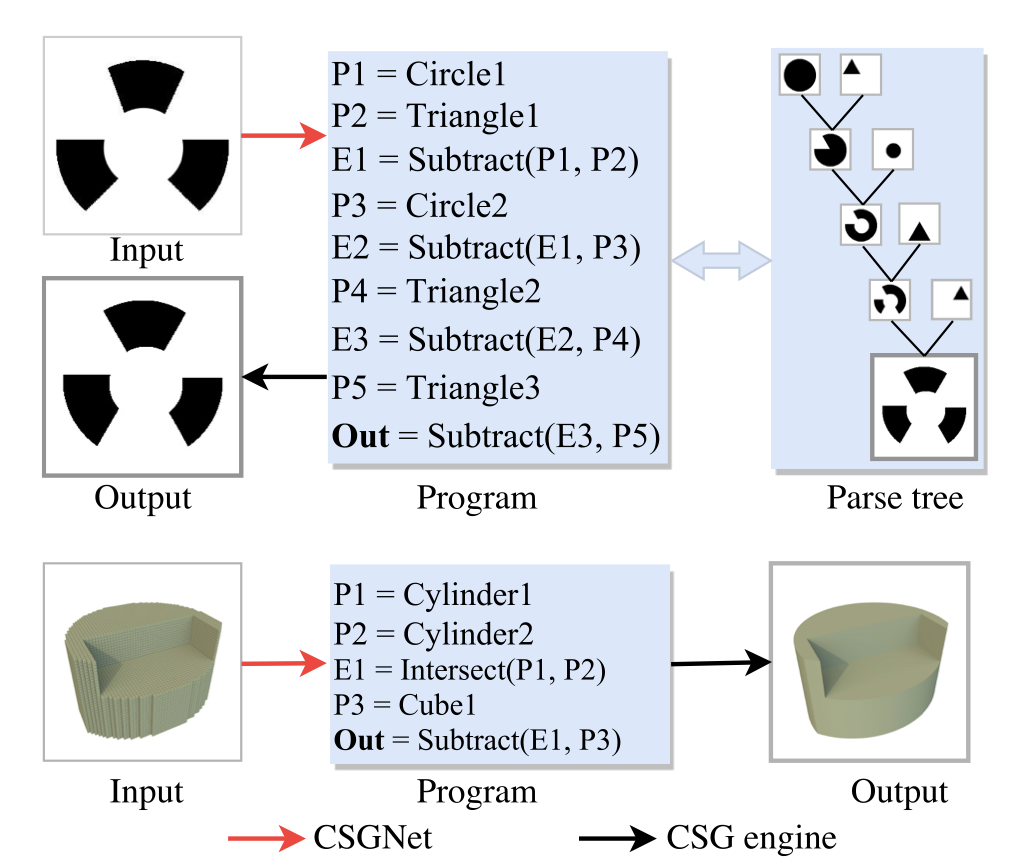
\includegraphics[width=0.8\textwidth]{figures/csgnetinput.png}
    \caption{The CSGNet pipeline for visual program induction. This illustrates the transition from unstructured geometric data (pixels and voxels) to symbolic logic. A neural parser (red arrows) ``lifts'' the raw geometry into an interpretable, hierarchical program and its corresponding parse tree, while a symbolic engine (black arrows) ensures the program remains an accurate, executable representation of the original shape. Original Figure from \cite{CSGNet}}
    \label{fig:csgnetinput}
\end{figure}

While these methods effectively reverse-engineer CAD-like instructions, they are often limited to producing ``flat'' sequences or fixed-depth trees. Such representations typically lack high-level procedural logic, failing to capture recursive structures, loops, or complex conditional variables \cite{Du2018, ren2021}. To mitigate the complexity of irregular tree structures, CSG-Stump \cite{ren2021} was proposed to provide a more computationally efficient optimization formulation (see \autoref{fig:csgstump}). By replacing the arbitrary, deep topology of standard CSG with a structured, fixed-depth ``stump'', the model enables more stable gradient-based learning while maintaining the ability to represent intricate geometric assemblies.

\begin{figure}[htbp]
    \centering
    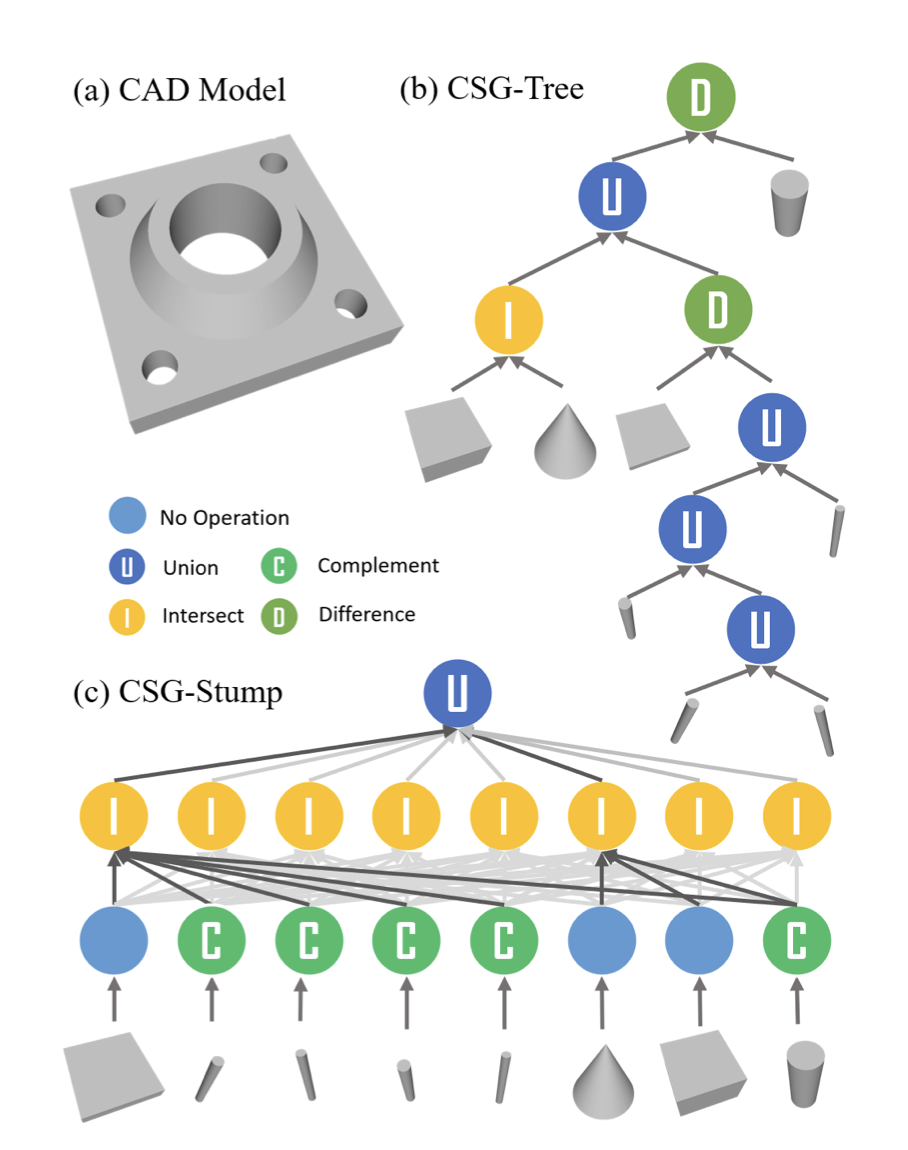
\includegraphics[width=0.8\textwidth]{figures/csgstump.png}
    \caption{A comparison between the irregular topology of a traditional CSG tree (b) and the structured CSG-Stump representation (c). The latter provides a fixed-depth architectural template that is significantly better suited for neural network optimization and end-to-end differentiability. Original Figure from \cite{ren2021}.}
    \label{fig:csgstump}
\end{figure}

To bridge the gap between rigid primitives and organic real-world shapes, recent literature has shifted toward representing object parts as \textbf{subroutines defined by implicit functions}. ProGRIP \cite{ProGRIP}, for instance, addresses the limitations of predefined primitive libraries by employing an unsupervised matching objective to identify repeatable ``macros'' within a shape. This allows for modeling geometric similarities as reusable subroutines, significantly improving reconstruction fidelity without requiring manual program labels. By leveraging neural implicit functions, these frameworks retain high-frequency details that are typically discarded in voxelized or purely primitive-based pipelines.

In the \textbf{neurally-guided search}, a policy network observes the current geometric state and predicts the most probable subsequent symbolic command. As illustrated in \autoref{fig:Tian2019working}, frameworks like L-IE \cite{Tian2019} utilize a differentiable program executor to bridge the gap between discrete symbolic code and continuous raw geometry. This enables an end-to-end training loop where the network is optimized to minimize the geometric reconstruction loss by back-propagating errors through the execution floor. By combining these executors with search algorithms like those in DreamCoder \cite{DreamCoder}, models can navigate complex program manifolds more efficiently than stochastic or brute-force search methods \cite{Ellis2019, Tian2019}.

\begin{figure}[htbp]
    \centering
    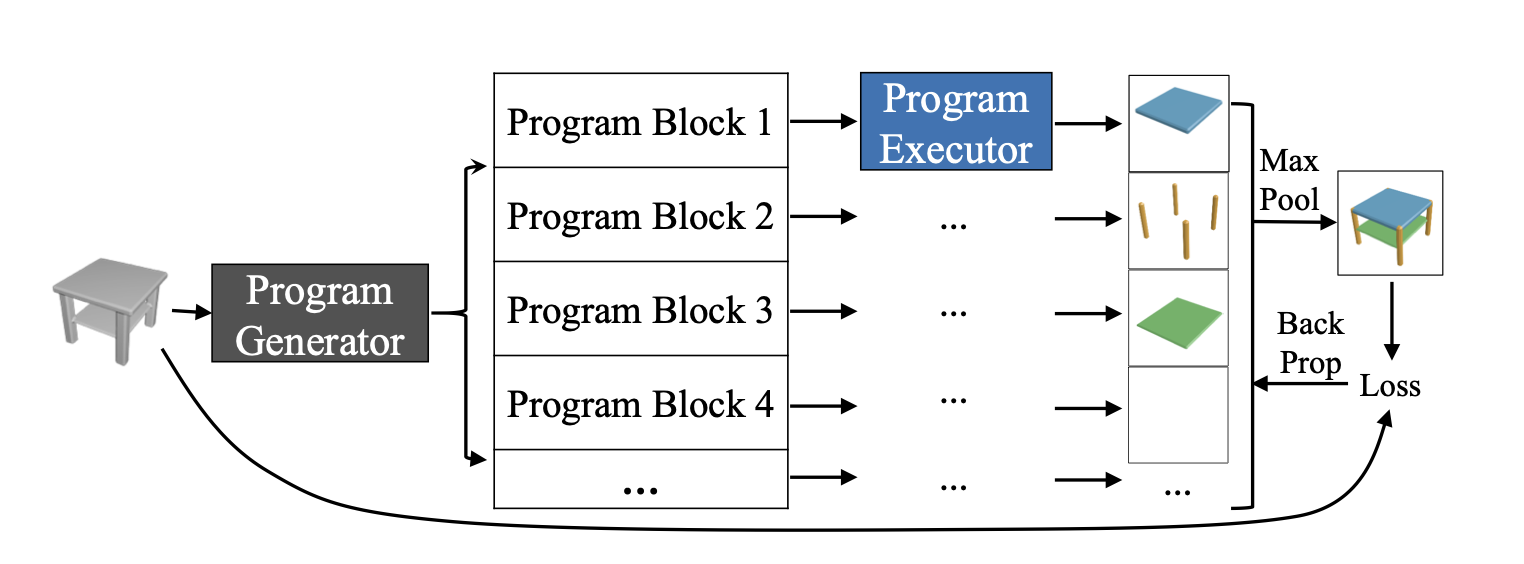
\includegraphics[width=0.8\textwidth]{figures/Tian2019working.png}
    \caption{The Learning-to-Infer-and-Execute (L-IE) framework \cite{Tian2019}. A program generator predicts symbolic blocks, which are then rendered into geometry by a differentiable executor. This allows the system to back-propagate geometric reconstruction errors directly through the program structure to update the neural weights. Original Figure from \cite{Tian2019}.}
    \label{fig:Tian2019working}
\end{figure}

Despite the progress in neurally-guided search and implicit representations, a significant limitation remains in resolving complex, non-linear parametric dependencies without manual symbolic templates. Building upon these neurosymbolic foundations, this thesis utilizes the neural modeling of parametric data distributions guided by Local Intrinsic Dimensionality to further explore the discovery of non-linear geometric abstractions.

\section{Automatic Abstraction and Macro Discovery}

Automatic abstraction focuses on decomposing complex structures into modular and reusable components \cite{Simon1996}. Within program induction, this is typically formalized as constructive induction. The goal is to expand a base language with higher-order macros that capture recurring structural regularities found across a dataset. Early work in this domain established that data compression provides a powerful inductive bias for identifying ``good'' representations \cite{Rissanen1978}, a concept that has evolved from Inductive Logic Programming (ILP) to modern neurosymbolic frameworks.

A central concept in modern abstraction discovery is \textit{multitask library induction}, where the system grows its own toolkit by identifying shared structure across disparate tasks. The Exploration-Compression (EC) algorithm \cite{Dechter2013} and its successor, DreamCoder \cite{DreamCoder}, utilize a ``Wake-Sleep'' cycle to iteratively solve problems and refactor the resulting programs into a common library. As illustrated in Figure \ref{fig:dreamcodercycle}, this cycle uses neural architectures to guide the synthesis of symbolic code, combining the formal structure of a program with the learning efficiency of a neural network.

\begin{figure}[htbp]
    \centering
    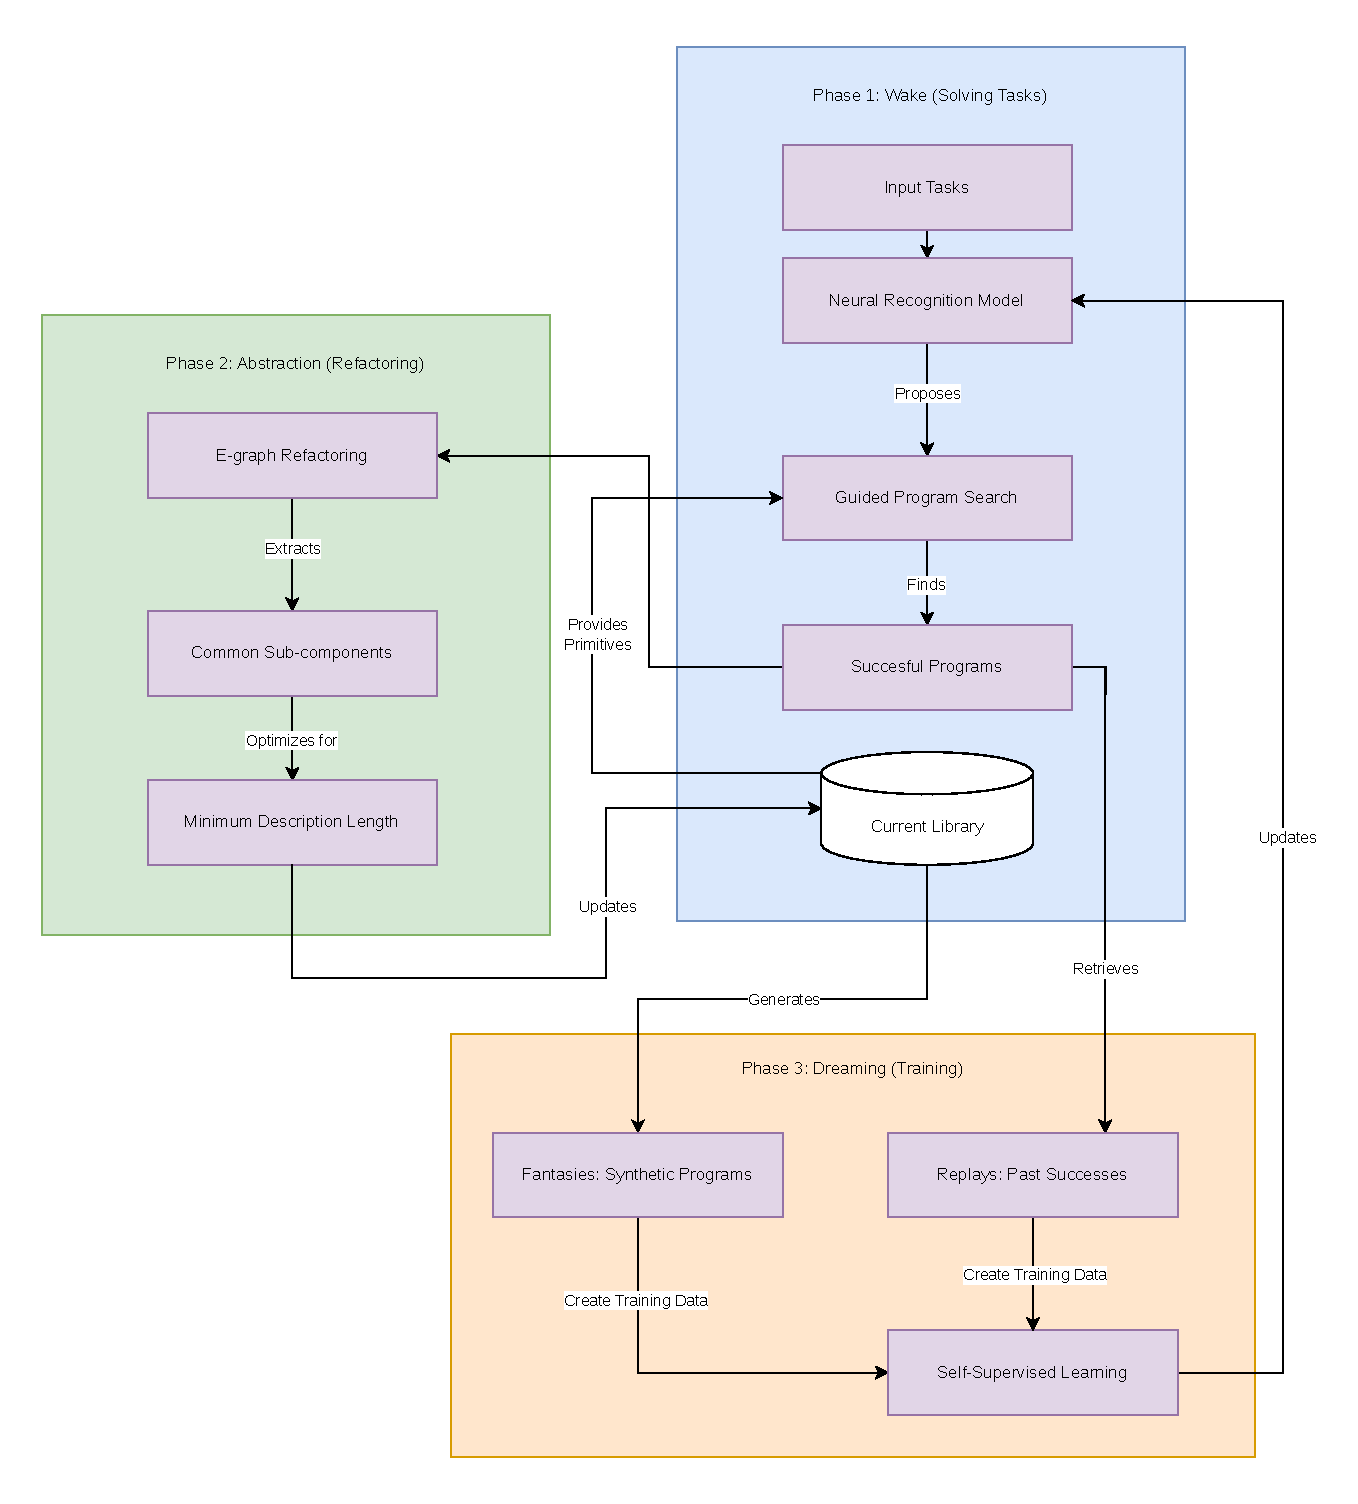
\includegraphics[width=0.85\textwidth]{figures/dcdrawio.pdf}
    \caption{The DreamCoder iterative learning cycle: (1) In the \textbf{Wake} phase, the system performs neural-guided search to synthesize programs for given tasks; (2) the \textbf{Abstraction} phase refactors these solutions using E-graph matching to expand the library with modular primitives that maximize MDL compression; and (3) the \textbf{Dreaming} phase trains the recognition model on self-generated ``hallucinations'' (synthetic tasks) to improve search efficiency for subsequent iterations. Original Figure from \cite{DreamCoder}, but simplified for clarity.}
    \label{fig:dreamcodercycle}
\end{figure}

While these systems traditionally relied on stochastic local search (e.g., Genetic Programming \cite{Koza1992}) or hierarchical Bayesian models \cite{Liang2010}, they often struggled with the combinatorial explosion of the program search space. This wake-sleep process creates a hierarchy of abstractions where complex, multi-step operations are condensed into single library calls, effectively reducing the search space for large-scale, high-dimensional problems.

To address these scaling challenges, recent research has diverged into two primary algorithmic lineages: \textit{deductive refactoring} and \textit{guided top-down synthesis}. Deductive systems like Babble \cite{Cao2023} leverage the structural sharing of E-graphs combined with anti-unification to discover shared sub-structures across a program corpus, which enables the identification of abstractions modulo semantic equivalences. In contrast, the Stitch framework \cite{Bowers2023} improves synthesis efficiency by utilizing a top-down, branch-and-bound search strategy. By employing a compression upper-bound heuristic to prune the search space, Stitch achieves orders-of-magnitude speedups over previous bottom-up methods while maintaining formal optimality guarantees on the discovered library.

\begin{figure}[htb]
    \centering
    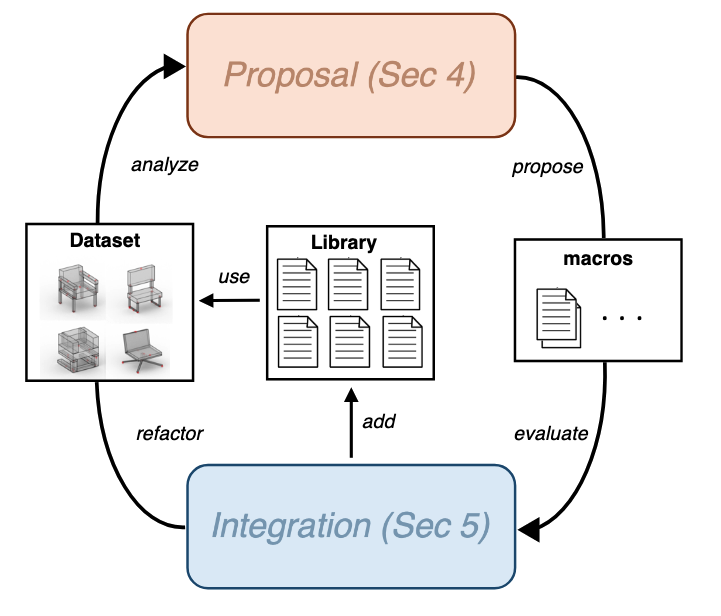
\includegraphics[width=0.8\textwidth]{figures/ShapeModPhases.png}
    \caption{The ShapeMOD discovery and integration loop \cite{ShapeMOD}. The framework identifies recurring program patterns in the input dataset to propose candidate macros (Proposal phase), which are then evaluated and integrated into the DSL library to maximize global compression through programmatic refactoring. Original Figure from \cite{ShapeMOD}.}
    \label{fig:ShapeModPhases}
\end{figure}

In the domain of geometric modeling, the discovery problem is further complicated by the presence of continuous parameters. ShapeMOD \cite{ShapeMOD} addresses this (see \autoref{fig:ShapeModPhases}) by extending macro discovery to imperative, statement-based 3D programs. It operates on the principle of minimizing the total Description Length of a shape collection by reducing both the number of function calls and the count of free parameters. An important contribution of ShapeMOD is its ability to identify linear relationships between continuous attributes, allowing for the creation of parametric macros that generalize across diverse objects. However, as it targets imperative languages like ShapeAssembly, it faces challenges in structural optimization, the authors note that E-graphs and similar version-space structures are difficult to apply to imperative code due to the complexities of semantic line re-ordering. This motivates the need for a more formal analysis of the underlying parameter distributions to identify the true degrees of freedom required for accurate modeling.

\section{Intrinsic Dimensionality Estimation}\label{rel_work_estimation}

The estimation of Intrinsic Dimensionality (ID) involves approximating the minimal number of variables $d$ required to represent an underlying manifold $\mathcal{M}$ from a set of discrete samples $X \subset \mathbb{R}^D$, where $D$ is the ambient dimension. While global estimators assume a uniform dimension for the entire dataset, \textbf{Local Intrinsic Dimensionality (LID)} techniques identify the varying degrees of freedom that often exist across different regions of a complex manifold \cite{IntrinsicDim}. These estimators are typically categorized into four primary families based on their geometric, topological, or statistical characterization of data.

Projection-based methods utilize the spectral properties of the local data distribution. \textit{Local PCA (lPCA)} identifies dimensionality by locating a significant gap in the eigenvalue decay of local covariance matrices \cite{Fukunaga1971, fanlpca}. This approach is computationally efficient and provides a direct spectral representation of the local subspace. However, lPCA is sensitive to manifold curvature, as high-curvature non-linear structures are frequently misinterpreted as higher-dimensional linear hyperplanes.

Geometric and Graph-based methods approximate the manifold topology by treating the data as a discrete graph. Algorithms such as \textit{Isomap} utilize geodesic distances to identify the underlying coordinates of the manifold \cite{Tenenbaum2000}. While useful for global manifold unfolding, these methods are sensitive to noise and the ``short-circuit'' problem, where erroneous edges between distant branches distort the estimated dimension.

Fractal and Expansion-based methods analyze how the number of point pairs within a radius $r$ scales as $r$ increases. A prominent algorithm in this family is the \textit{Correlation Dimension} \cite{Grassberger1983}. The principal disadvantage of expansion-based logic is high sample complexity. In high-dimensional spaces, these estimators require an exponentially large number of points to achieve stable convergence \cite{Kegl2002}.

Nearest-Neighbor (NN) methods model ID as a parameter of the distance distribution rather than a spatial volume. The \textit{Maximum Likelihood Estimator} assumes that the data points follow a local Poisson process \cite{Levina2004MaximumLE}. A limitation of the MLE is the reliance on absolute distances, which assumes a locally constant density. This is frequently violated by the characteristic density fluctuations in shape datasets. Another method is \textit{TWO-NN}, which ignores absolute distances in favor of the ratio between the first and second nearest neighbors \cite{faccotwonn}. This scale-invariant approach remains robust against variations in density and curvature.

In the proposed framework, these techniques serve as complementary lenses. By reconciling the spectral insight of lPCA with the statistical robustness of TWO-NN, the system identifies the irreducible degrees of freedom in shape parameters to establish the architectural constraints for the neural abstractions.

\section{Neurosymbolic Integration and Guidance}

The integration of symbolic rewriting engines with neural guidance has established a powerful logic for solving complex optimization and synthesis tasks across diverse scientific domains. In these frameworks, E-graphs are often used to manage the combinatorial explosion of the version space, while data-driven models provide the heuristics necessary to identify optimal solutions. 

A primary application of E-graph-based expression optimization is found in the domain of numerical analysis. For instance, \textit{Herbie} \cite{Panchekha2015} addresses the accumulation of rounding errors in floating-point arithmetic. Rather than applying a fixed sequence of transformations, it represents a vast space of mathematically equivalent expressions within an E-graph. By sampling input points to identify regions of high precision loss, Herbie discovers non-obvious rewrites that improve the numerical accuracy of mathematical formulas. In this context, the E-graph serves as a non-destructive environment for algebraic exploration, allowing the system to locate stable alternatives that might be missed by manual rearrangement.

This strategy of automated symbolic refactoring extends to hardware-level optimizations in deep learning. The TASO framework \cite{Jia2019} utilizes E-graphs to optimize computation graphs by automatically generating and formally verifying graph substitutions. Unlike traditional compilers that rely on manually authored rules, TASO performs a cost-based backtracking search over the E-graph to discover optimized structural layouts. This demonstrates that E-graphs can effectively bridge the gap between high-level algorithmic descriptions and low-level execution efficiency by treating optimization as a search for identity-preserving replacements.

However, as the program space grows, symbolic engines often require an external guiding signal to remain manageable. \textit{DeepCoder} \cite{Balog2017} exemplifies the use of ``neural guidance'' in program induction. Instead of relying purely on enumerative search, it trains a deep network to predict high-level program properties from input-output examples. These predictions are then used to reorder the search space, allowing symbolic solvers to find solutions an order of magnitude faster. This hybrid method, where a neural component provides global intuition and a symbolic component ensures local correctness, is central to the structural discovery process used in this thesis.

\section{The ShapeCoder Framework}

The framework presented in this thesis is inspired by ShapeCoder \cite{ShapeCoder}, which discovers a library of abstractions directly from unstructured geometric primitives. A core challenge in this domain is that, in general, there are many different programs $p$ that can recreate a given shape $d$. The fundamental goal of the ShapeCoder framework is to find the ``best'' possible programs using functions from a library $\mathcal{L}$ to recreate all shapes $d$ within a dataset $\mathcal{D}$. Taking a functional DSL as a base, ShapeCoder leverages the efficiency of E-graphs to navigate the version space of equivalent programs, a task that was computationally difficult in previous imperative frameworks like ShapeMOD. The system receives three primary inputs: a base functional library $\mathcal{L}$, a dataset of shapes $\mathcal{D}$ (represented as unstructured primitive clouds), and an MDL-guided objective function $\mathcal{F}$.

ShapeCoder's lifecycle is divided into four interleaved phases designed to minimize $\mathcal{F}$. The \textbf{Dream} phase samples expressions from the current library to train a recognition network (\autoref{fig:screcogdreamwake}). The \textbf{Wake} phase then uses this network to infer programs $\mathcal{P}$ that explain the shapes in $\mathcal{D}$. These programs are passed to the \textbf{Proposal} phase, which identifies recurring structural fragments to generate candidate abstraction functions. Finally, the \textbf{Integration} phase evaluates these candidates and updates $\mathcal{L}$ to reflect the most effective abstractions. By converting the problem of shape induction into a functional refactoring task, ShapeCoder can discover deep hierarchies that are more compact and editable than the ``flat'' programs produced by earlier VPI methods.

\subsection{Optimization Objective}

The success of the discovery process is calculated by the objective function $\mathcal{F}(\mathcal{L}, \mathcal{P})$, which measures the trade-off between library complexity and the average program complexity across the dataset. Guided by the MDL principle, the system favors shorter, more compact representations. The joint objective for a library $\mathcal{L}$ and a set of programs $\mathcal{P}$ is expressed as:

\begin{equation}
    \mathcal{F}(\mathcal{L}, \mathcal{P}) = \frac{1}{|\mathcal{P}|} \sum_{p \in \mathcal{P}} \left[ \left( \sum_{\tau \in T} \lambda_{\tau} \cdot \tau(p) \right) + \lambda_{e} \cdot \mathrm{err}(p, d) \right] + \sum_{f \in \mathcal{L}} \omega(f)
\end{equation}

Here, the term within the square brackets represents the total description length of an individual program $p$. The structural cost is calculated as a weighted sum over all token types $\tau \in T$ (such as functions, geometric primitives, or parameters), where $\tau(p)$ denotes the frequency of tokens of type $\tau$ in the program and $\lambda_{\tau}$ is its associated weight. 

To ensure high reconstruction fidelity, the model uses a geometric error function $\mathrm{err}(p, d)$. Here, $d$ represents the ground-truth target shape from $\mathcal{D}$ that program $p$ intends to reconstruct. If the distance between the program output and the target shape $d$ exceeds a specific threshold, the objective returns $\infty$. Otherwise, the error is added to the program complexity with weight $\lambda_{e}$. These program-specific costs, comprising both structural complexity and reconstruction error, are averaged across the entire set $\mathcal{P}$ via the normalization factor $1/|\mathcal{P}|$.

Finally, the global library complexity is measured via the weighting scheme $\omega(f)$ for each function $f \in \mathcal{L}$. This allows the system to penalize overly complex abstractions, for instance by increasing the weight $\omega$ for functions that consume a large number of input parameters. By balancing these averaged program costs against the global library cost, ShapeCoder identifies abstractions that provide the most efficient explanation for the structural regularities found in the dataset.

\begin{figure}[htbp]
    \centering
    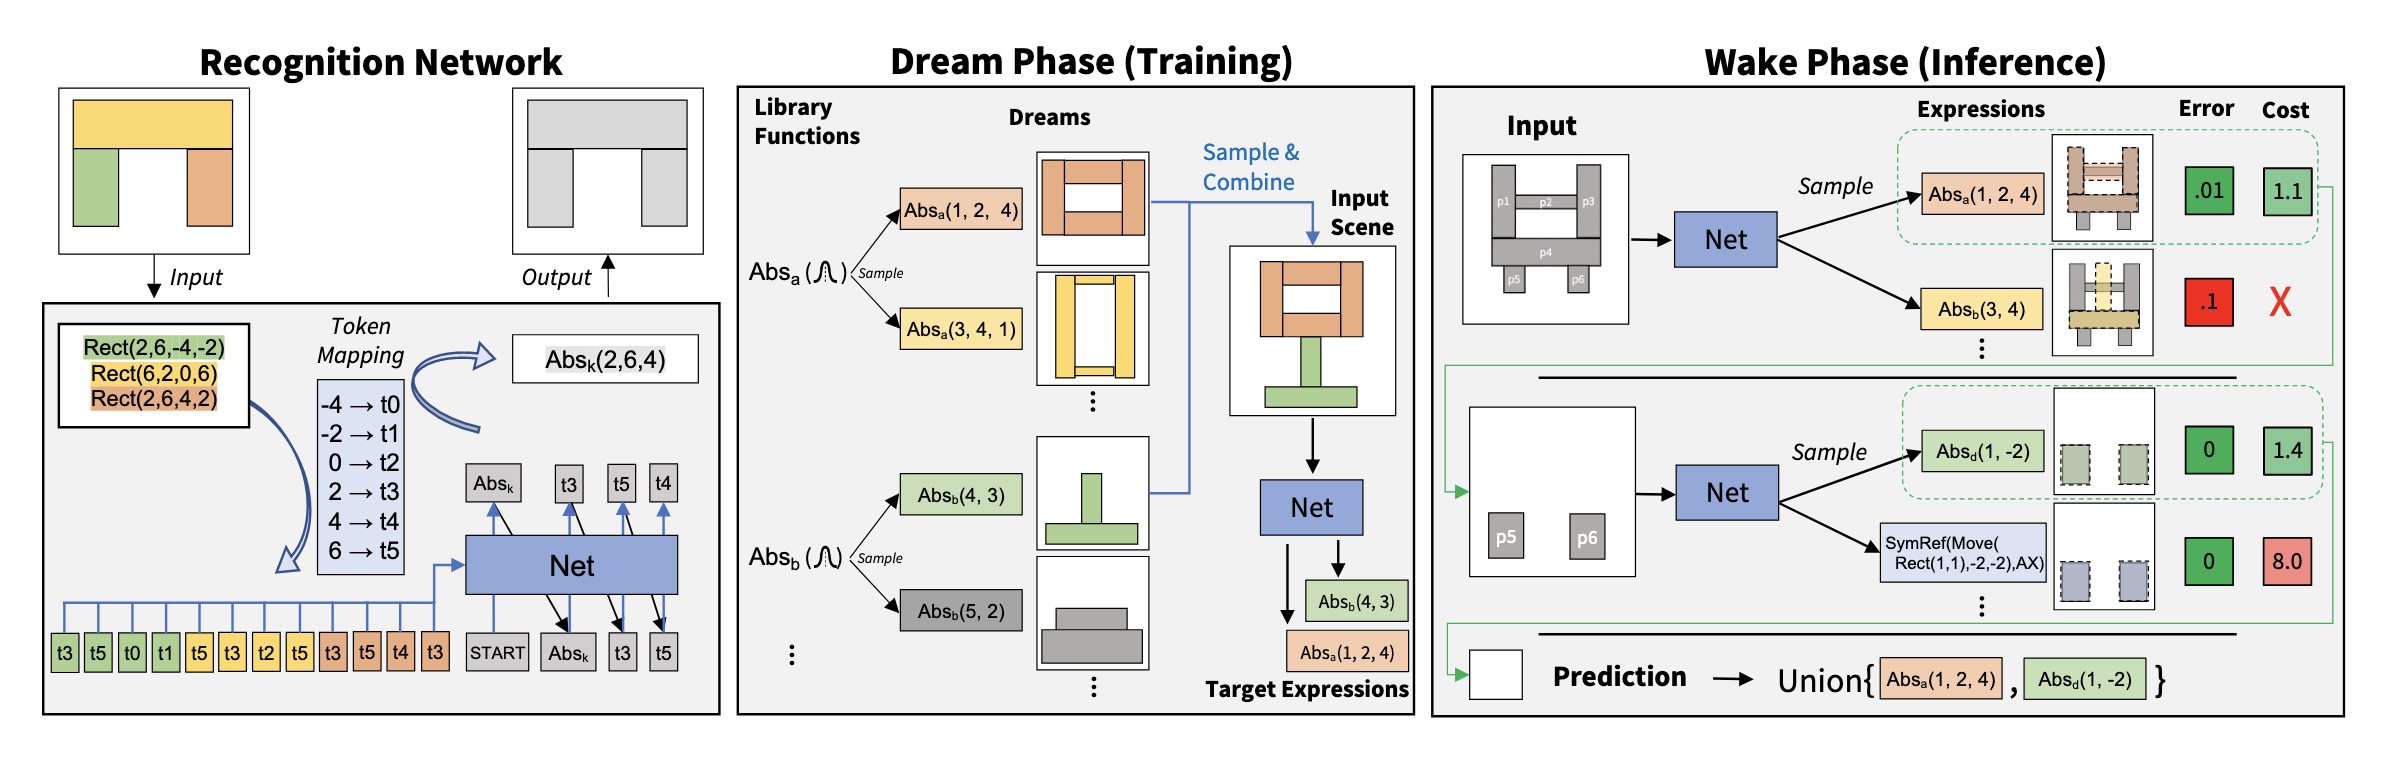
\includegraphics[width=\textwidth]{figures/screcogdreamwake.png}
    \caption{Key components of the ShapeCoder framework. The Transformer-based recognition network (left) processes primitives to predict program sequences. During the dream phase (middle), the network is trained on synthetic data sampled from the library. In the wake phase (right), the network iteratively explains target shapes by selecting library expressions that minimize the cost objective. Original Figure from \cite{ShapeCoder}}
    \label{fig:screcogdreamwake}
\end{figure}


\subsection{Recognition Network}
To navigate the vast search space of possible programs, ShapeCoder utilizes a recognition network designed to propose expressions from the library $\mathcal{L}$ that explain subsets of the input geometry. As illustrated in Figure \ref{fig:screcogdreamwake}, the network is implemented as a Transformer decoder \cite{Vaswani2017} that autoregressively predicts sequences of program tokens. The model is conditioned on an encoding of the input primitives. For a scene containing $M$ primitives each defined by $K$ parameters, the network attends over $K \times M$ conditioning tokens. This bottom-up approach allows the network to identify and explain partial structures within complex inputs, enabling ShapeCoder to operate without a curriculum of examples, a significant advancement over previous iterative discovery frameworks \cite{DreamCoder, ShapeMOD}.

A critical challenge in this symbolic induction task is handling continuous, real-valued parameters within a discrete Transformer framework. ShapeCoder addresses this through a scene-specific token mapping procedure. For each input scene, the system extracts all real-valued primitive parameters, rounds them to a fixed precision (e.g., two decimal places), and sorts them to create a unique, scene-local vocabulary. This mapping is used both to form the conditioning tokens and to convert the network's autoregressive predictions back into precise numerical values. By effectively transforming a regression problem into a discrete sequence prediction task, the recognition network can propose complex, parametrically accurate code snippets directly from unstructured geometry.

\subsection{Dream Phase}
The \textit{Dream} phase generates the synthetic training data required for the recognition network to learn the mapping between geometry and code (\autoref{fig:screcogdreamwake}, middle). For each function $f \in \mathcal{L}$, ShapeCoder generates $N_D$ ``dreams'' by sampling random instantiations of the function's parameter slots. To ensure geometric validity, the system employs rejection sampling to filter out invalid outputs, such as those that exceed scene boundaries, contain negative dimensions, or possess redundant primitive containment.

Since target shapes in $\mathcal{D}$ are typically composed of multiple structural sub-units, training solely on single-function dreams would limit the network's generalization. To address this, ShapeCoder constructs \textbf{composite scenes} by merging $N_C$ independently sampled dreams into a single input canvas. This creates a one-to-many training process. For a given composite scene, the network is trained in a supervised fashion to predict each of the $N_C$ corresponding program sequences. By ensuring every function in the library is represented in at least $N_D$ training targets, the recognition network is robustly updated via maximum likelihood estimation, allowing it to learn how to decompose complex, unstructured inputs into explainable programmatic fragments.

\subsection{Wake Phase}

The \textit{Wake} phase aims to infer a program $p$ that explains an input shape $d$ while minimizing the objective function $\mathcal{F}$ using the trained recognition network. As shown in Figure \ref{fig:screcogdreamwake}, the process begins by initializing a scene with the primitives of $d$ and proceeds iteratively. In each iteration, the recognition network is conditioned on the current primitives and samples a large set of candidate expressions from $\mathcal{L}$ until a specified timeout.

For each sampled expression $e$, the system evaluates its cost under $\mathcal{F}$, specifically normalizing the structural complexity of $e$ by the number of primitives it successfully explains. Expressions that fail to reconstruct a valid subset of the input primitives incur high geometric error, causing $\mathcal{F}$ to return $\infty$. ShapeCoder greedily selects the expression $e^*$ with the lowest normalized cost, removes the primitives covered by $e^*$ from the input scene, and feeds the updated canvas back into the network. This cycle continues until the entire input scene has been explained; to guarantee convergence, a ``naive'' expression that describes a single primitive using its exact parameters is always available as a fallback.

Finally, the complete program $p$ for shape $d$ is formed by applying the appropriate combinator operations (e.g., \texttt{Union}) across all selected $e^*$. To prevent the system from ``forgetting'' high-quality solutions found in previous rounds, ShapeCoder maintains a persistent program set $\mathcal{P}$. In each round, newly discovered programs are merged with existing solutions through a greedy replacement search, ensuring that only the program variants that optimize the global objective $\mathcal{F}$ are retained.



\subsection{Proposal Phase}

\begin{figure}[htb]
    \centering
    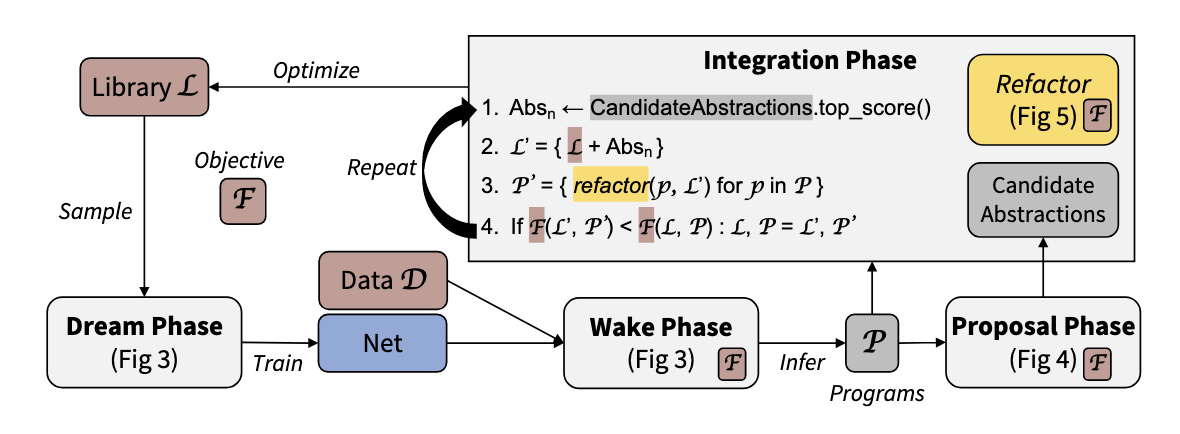
\includegraphics[width=\textwidth]{figures/scproposalintegration.png}
    \caption{The iterative discovery and integration loop in ShapeCoder. Candidate abstractions are proposed from current program solutions and integrated into the functional library $\mathcal{L}$ after a cost-based validation process. Original Figure from \cite{ShapeCoder}.}
    \label{fig:scproposalintegration}
\end{figure}


The goal of the \textit{Proposal} phase is to search the collection of inferred programs $\mathcal{P}$ for candidate abstractions that would minimize the global objective $\mathcal{F}$ if incorporated into the library $\mathcal{L}$ (\autoref{fig:scproposalintegration}, bottom-right). As solving this search problem globally is computationally intractable, ShapeCoder decomposes the process into manageable sub-problems by aggregating local solutions through a recursive sampling and clustering strategy. To generate an abstraction, the system must determine both its structural sequence (the functional fragments) and its parameterization (how inputs map to sub-functions). To factor out variations in expression ordering, ShapeCoder identifies potential structures by recording all singleton and paired combinations of sub-expressions found in $\mathcal{P}$, subsequently filtering out patterns that appear in less than 5\% of the dataset to ensure focus on generalizable regularities.

Once these potential structures are recorded, the phase iteratively samples a random structure and a subset of its observed parameterizations to form a cluster. A greedy search is then performed over this cluster to optimize a local version of $\mathcal{F}$ (\autoref{fig:scgreedy}), with the resulting candidate abstractions stored alongside their ``coverage set'' which is the specific subset of programs in $\mathcal{P}$ that can be simplified through their application. This search is guided by a score function that combines two key metrics: \textit{frequency} (the percentage of cluster instances where the abstraction applies) and \textit{gain} (the reduction in program description length). For a proposed abstraction $a$ and a program $p$, let $p_a$ denote the rewritten program. The gain is formally defined as:

\begin{figure}[htb]
    \centering
    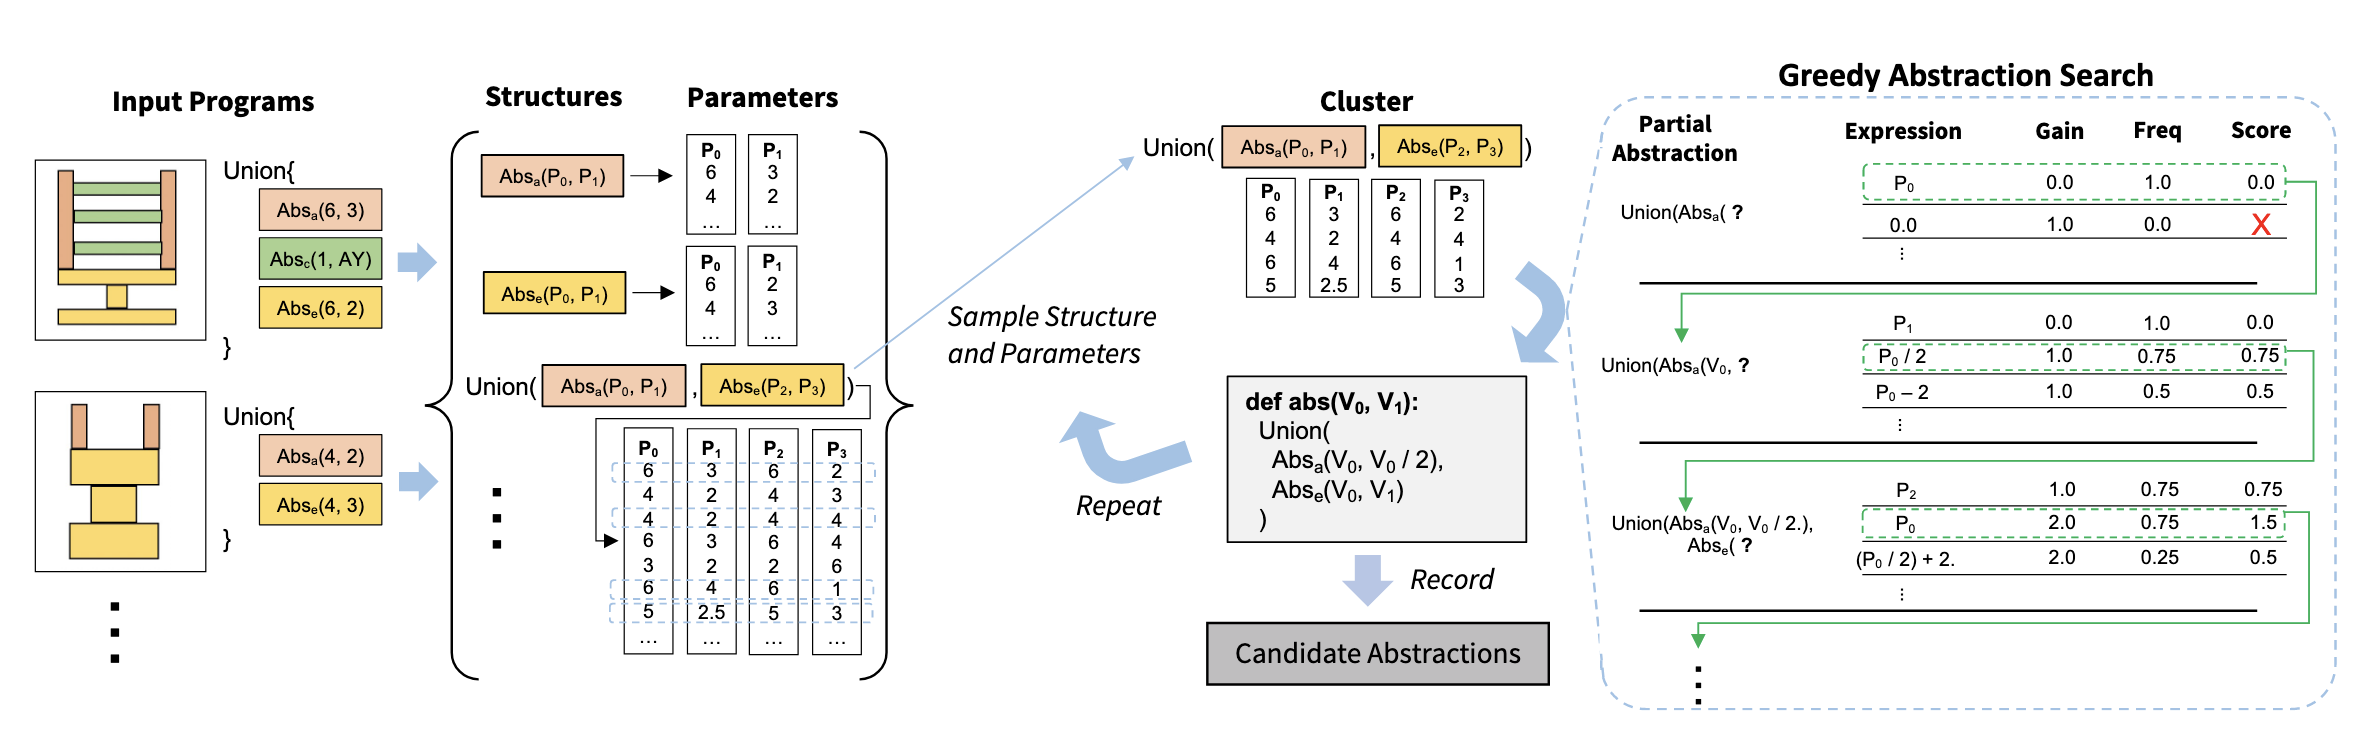
\includegraphics[width=\textwidth]{figures/scgreedy.png}
    \caption{Symbolic Parameter Discovery Process. ShapeCoder aggregates recurring structural fragments into clusters and attempts to 'solve' their parametric slots by iterating through a predefined library of symbolic templates (e.g., $P_1 = P_0/2$). This discrete search process identifies high-score candidates that maximize both usage frequency and description length gain. Original Figure from \cite{ShapeCoder}.}
    \label{fig:scgreedy}
\end{figure}

\begin{equation}
    \text{gain}(a) = \sum_{\tau \in T} \lambda_\tau \cdot (\tau(p) - \tau(p_a))
\end{equation}
where $\tau(p)$ represents the frequency of tokens of type $\tau \in T$ in the program $p$, and $\lambda_\tau$ is the token-specific weight as defined in the global objective function.

For each parameter slot in the structure, ShapeCoder evaluates a variety of instantiation strategies including reusing previously defined parameters, assigning static constants, or introducing new free variables and selects the configuration that maximizes the joint frequency-gain score. For real-valued parameters, the system iterates through a preference-ordered list of parametric relationships to identify the most compact symbolic representation. This process results in a diverse set of candidate abstractions that are passed to the integration phase for global evaluation.

\subsection{Integration Phase}
The final stage of a ShapeCoder round is the \textit{Integration} phase, which identifies the optimal library $\mathcal{L}'$ and program set $\mathcal{P}'$ to minimize the global objective $\mathcal{F}$ (\autoref{fig:scproposalintegration}, top-right). This phase leverages a specialized \textit{refactor} operation that utilizes E-graphs (equivalence graphs) to efficiently identify minimal-cost equivalent programs under different library variants. The process begins by recording the current objective value $\mathcal{F}(\mathcal{L}, \mathcal{P})$ and iteratively attempting to improve it. In each step, a new library variant $\mathcal{L}'$ is proposed by adding a top-ranked candidate abstraction $a$ from the proposal phase. The system then generates a new program set $\mathcal{P}'$ by refactoring every program $p \in \mathcal{P}$ using the functions in $\mathcal{L}'$. 

Since evaluating a new library is computationally expensive, requiring a full refactor of the entire dataset, the system restricts the search to a small number ($N_A$) of high-scoring candidates. To maintain the accuracy of the score heuristic, the system discounts the frequency of abstractions that overlap on the same coverage set of primitives. To prevent the search from stalling in local minima, ShapeCoder also considers more complex library transformations. If adding an abstraction $a$ fails to improve $\mathcal{F}$ in isolation, the system identifies the set of existing functions $f_{dec}$ whose usage frequency decreased significantly in the new program set $\mathcal{P}'$. It then evaluates a variant $\mathcal{L}_{dec} = \{ \mathcal{L} \cup \{a\} \setminus f_{dec} \}$, allowing new, more efficient abstractions to replace older, less effective ones. Finally, the integration phase concludes by testing the removal of each function $f \in \mathcal{L}$ individually to prune redundant components. The best-performing library is then passed to the subsequent Dream phase, beginning the next cycle of discovery.

\subsection{Refactoring with E-Graphs}


To determine when and where discovered abstractions can be applied, ShapeCoder utilizes a specialized \textit{refactor} operation. This operation takes an input program $p$ and searches for an equivalent representation $p^*$ that minimizes the objective function $\mathcal{F}$. This vast search space is navigated using E-graphs (equivalence graphs) and a novel conditional rewriting scheme (\autoref{fig:screfactor}). E-graphs are data structures that represent large sets of equivalent programs through a compact forest of \textit{e-nodes}, representing functional terms, which are grouped into \textit{e-classes} to denote semantic equivalence. By iteratively applying rewrite rules, transformations that preserve program behavior the system can represent exponentially many program variations without a corresponding explosion in memory usage. Once the graph is sufficiently expanded, a greedy extraction algorithm identifies the lowest-cost program from the root e-class.

\begin{figure}[htb]
    \centering
    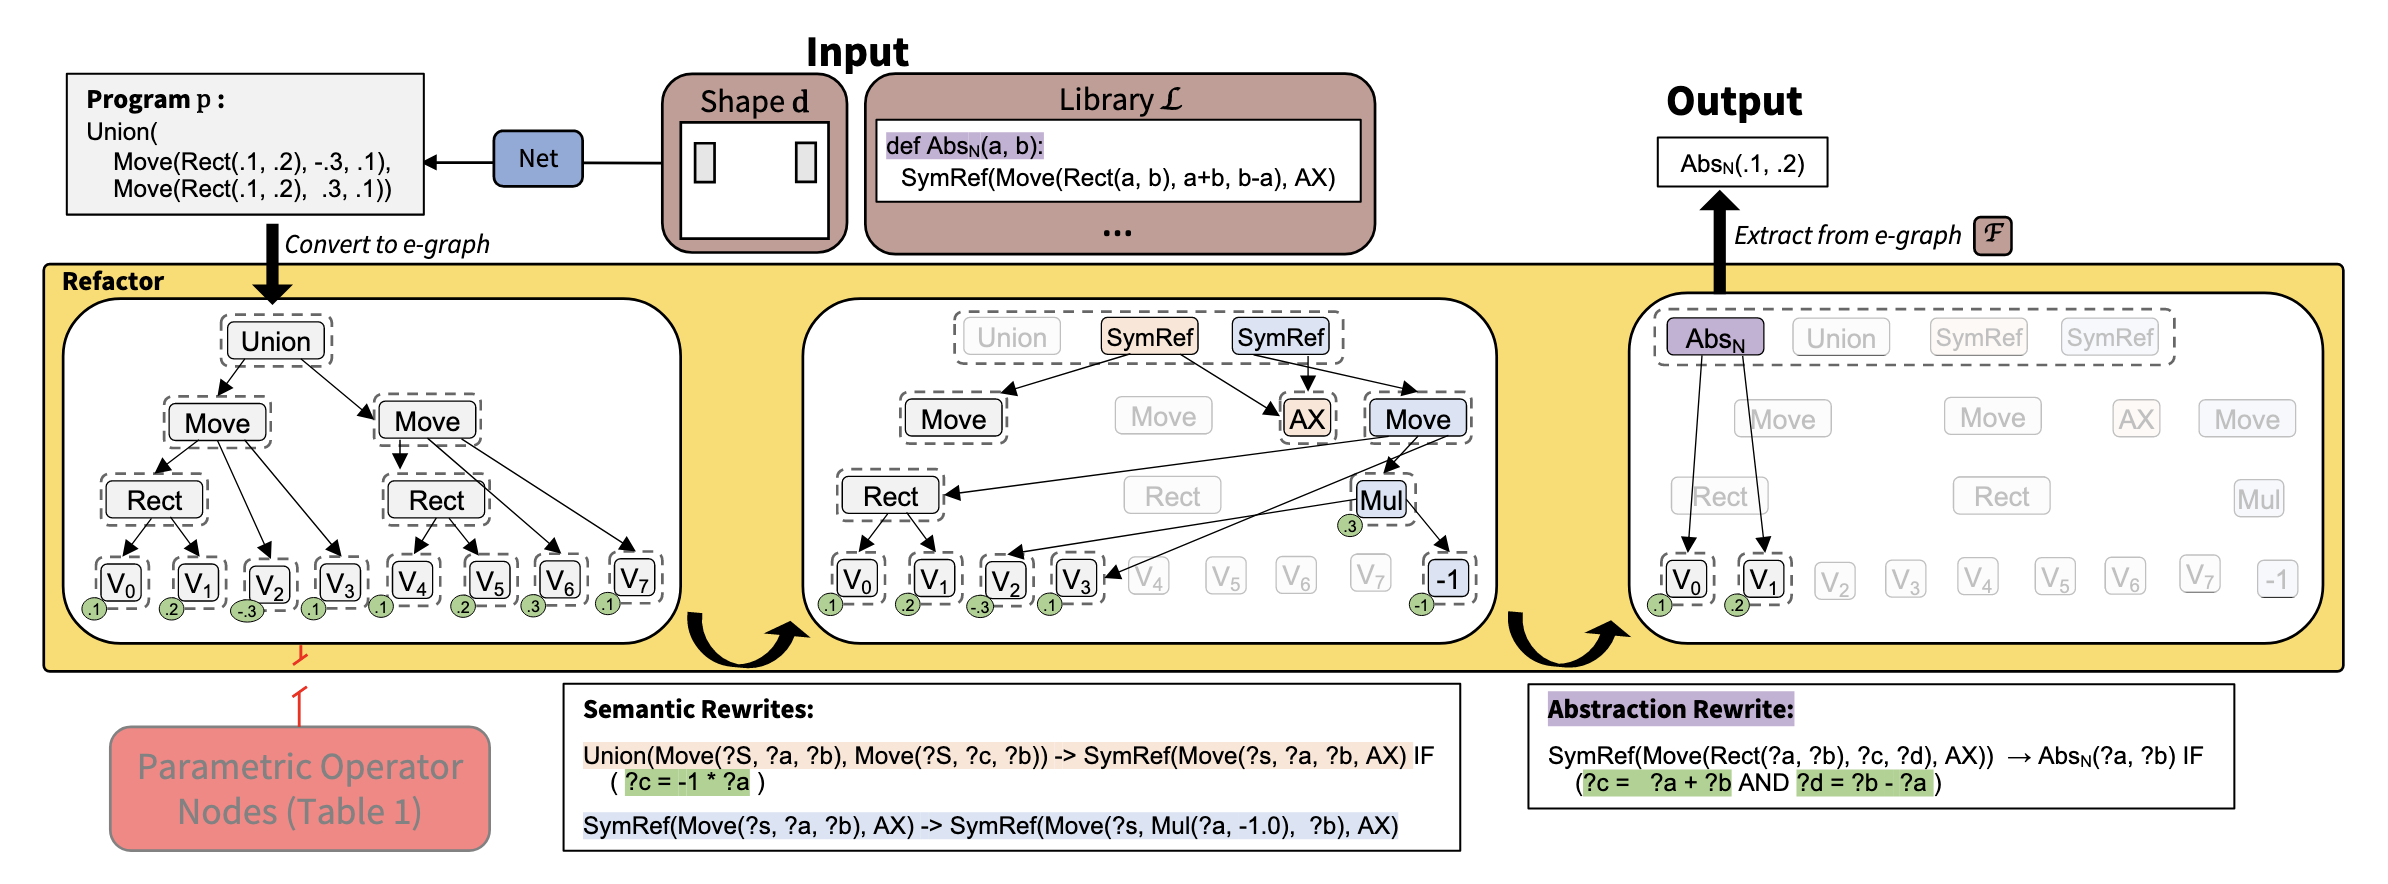
\includegraphics[width=\textwidth]{figures/screfactor.png}
    \caption{Automatic Programmatic Refactoring via E-graphs. Input programs are lifted into a version-space representation where real-valued parameters are replaced by symbolic variables. The graph is iteratively expanded through semantic and abstraction-specific rewrite rules, identifying equivalent representations across the global library. ShapeCoder employs a conditional rewriting scheme to validate parametric constraints (green highlights) without an explosion in e-nodes for numeric operators. The final optimized program is extracted from the saturated graph based on the global cost $\mathcal{F}$. Original Figure from \cite{ShapeCoder}.}
    \label{fig:screfactor}
\end{figure}

The refactor process begins by lifting the input program, a step that replaces all real-valued parameters with independent variables ($V_0, V_1, \dots$). The system then sources two types of rewrites from the library: \textit{semantic rewrites}, which represent algebraic identities of the base DSL, and \textit{abstraction rewrites}, which define the structural conditions required to apply a newly discovered macro. A core innovation of ShapeCoder is its \textit{conditional rewrite} scheme, designed to overcome the limitations of traditional structural matching. Visual programs require matching on complex parametric relationships such as checking if one coordinate is the sum or difference of others which typically leads to a combinatorial explosion in graph size if represented as standard e-nodes. 

ShapeCoder avoids this e-graph blowup by employing conditional rewrites that trigger only if a secondary parametric check passes. These checks are evaluated \textit{lazily}, ensuring that complex parametric logic is only computed once a viable structural candidate is identified. Furthermore, this scheme supports approximate matching by incorporating a maximum error threshold, enabling the discovery of abstractions even in the presence of imperfect geometric alignments. By decoupling structural matching from parametric validation, the refactor operation efficiently identifies the most compact symbolic representation for each shape in the dataset.


\section{Limitations: The Greedy Symbolic Gap}

Despite its structural flexibility, ShapeCoder is constrained by a fundamental bottleneck in its \textbf{Greedy Parametric Search}. When the system moves from identifying a common structural fragment (the slot-filling phase) to determining the relationships between its continuous parameters, it relies on a discrete, manually-curated library of symbolic templates.

We identify three primary flaws in this symbolic search strategy that serve as the technical motivation for this thesis:

\paragraph{The Symbolic Bottleneck} To capture a relationship, the system iterates through a fixed list of predefined equations, such as $y = x$ or $y = k \cdot x$. If a geometric dependency is non-linear or lacks a standard closed-form definition, the system fails to find a symbolic match within its predefined library. This lack of expressive capacity prevents the model from capturing complex dependencies that cannot be explicitly formulated via discrete symbolic primitives.

\paragraph{Combinatorial Explosion} The search for these relationships is performed greedily, checking parameters one-by-one or as a linear combination of others. As the complexity of the part signature increases, the number of possible parameter combinations grows exponentially. This forces the system to use aggressive pruning or heuristics, often causing it to miss subtle but global geometric regularities.

\paragraph{Parametric Bloat} When the search fails to find a symbolic identity, the system defaults to treating each variable as an independent free parameter. This results in programs that are uncompressed and noisy, as they fail to discard redundant degrees of freedom. Such programs are not only harder to edit but also fail to capture the true underlying data distribution of the shape.

To overcome these roadblocks, this thesis proposes replacing symbolic formulas with the neural modeling of continuous parametric data distributions. Crucially, we utilize Intrinsic Dimensionality (ID) as the formal tool to determine the manifold's dimension, informing exactly how many latent parameters the neural model requires to accurately capture the underlying geometric variation. By relying on data-driven manifolds rather than human-authored formulas, we bridge the Greedy Symbolic Gap and achieve a more flexible neurosymbolic representation.

%%%%%%%%%%%%%%%%%%%%%%%%%%%%%%%%%%%%%%%%%%%%%%%%%%%%%%%%%%%%%%%%%%%%%%%%%%%%%%%
% CHAPTER: METHODS
%%%%%%%%%%%%%%%%%%%%%%%%%%%%%%%%%%%%%%%%%%%%%%%%%%%%%%%%%%%%%%%%%%%%%%%%%%%%%%%

\chapter{Methods}\label{ch:methods}

\section{Problem Definition}
\label{sec:problem_definition}

The objective of our framework is to perform \textbf{neurosymbolic abstraction discovery}: identifying and modeling recurring geometric patterns within existing hierarchical shape representations. This process is formalized as a library learning problem where the system expands a base DSL with learned neural macros to improve the compression and editability of a dataset.

\subsection{Inputs}
The system operates on two primary inputs:
\begin{enumerate}
    \item \textbf{Hierarchical Program Dataset $\mathcal{D}$:} A collection of shapes where each $d \in \mathcal{D}$ is represented as a hierarchical program trace or \textit{symmetry hierarchy} (e.g., the output of the wake phase from ShapeCoder). Instead of a flat cloud of points, each shape is already organized as a symbolic tree whose nodes denote geometric segments (leaf nodes), adjacency relationships, or symmetry operations (e.g., reflectional or rotational groupings).
    \item \textbf{Base Library $L_{base}$:} A DSL defining the elementary operations of the system. This base library consists of a fixed set of geometric primitives (specifically unit \texttt{Box} components with semantic labels), linear transformations (\texttt{Translate}, \texttt{Rotate} via quaternions, and \texttt{Scale}), and structural combinators (\texttt{Union}) used to compose complex assemblies. Additionally, it includes higher-order symmetry operators like \texttt{SymRef} for reflection, \texttt{SymRot} for n-fold rotation, and \texttt{SymTrans} for n-fold translation which serve as the primitive building blocks for the initial hierarchies.
\end{enumerate}

\subsection{Outputs}
The induction process produces three primary outputs:
\begin{enumerate}
    \item \textbf{Abstraction Nodes $\mathcal{A}$:} A set of newly discovered library entries $\{a_1, a_2, \dots, a_m\}$ that capture recurring geometric patterns found across the hierarchies in $\mathcal{D}$. These ``neural macros'' replace rigid symbolic formulas or redundant parameter lists with learned manifold representations.
    \item \textbf{Optimized Library $L^*$:} The final library $L^* = L_{base} \cup \mathcal{A}$, which provides a more expressive and compact vocabulary for shape representation.
    \item \textbf{Compressed Dataset $P^*$:} A set of refactored programs where each $p \in P^*$ represents a shape from $\mathcal{D}$ using the abstractions in $L^*$. These programs are more compact than the originals, achieving a lower description length.
\end{enumerate}

\subsection{Objective Function: Minimum Description Length (MDL)}\label{sec:mdl_objective}

The discovery process is governed by the \textit{MDL} principle \cite{Rissanen1978}, which evaluates the fundamental trade-off between representational efficiency (compression) and reconstruction fidelity (distortion). We formalize this as a joint objective function $F(L, P)$ categorized into three primary costs:

\begin{equation}
    F(L, P) = \underbrace{\text{Cost}(L)}_{\text{Library Cost}} + \underbrace{\sum_{p \in P} \text{Cost}(p)}_{\text{Program Cost}} + \lambda \underbrace{\sum_{p \in P} \mathcal{L}_{\text{err}}(p)}_{\text{Error Penalty}}
\end{equation}

Where the individual components are defined as follows:

\begin{itemize}
    \item \textbf{Library Cost $\text{Cost}(L)$:} Represents the complexity of the global toolkit. It is defined as $\sum_{a \in L} w_a$, where $w_a$ serves as a fixed \textit{definition penalty} for each primitive or learned abstraction $a$ in the library. This term acts as a structural prior that penalizes over-fitting the library, ensuring that new abstractions are only incorporated if they provide a significant reduction in the global description length.
    
    \item \textbf{Program Cost $\text{Cost}(p)$:} Measures the complexity of an individual shape program $p$. For a program represented as a hierarchical tree of operations, the cost is calculated as:
    \begin{equation}
        \text{Cost}(p) = \sum_{n \in \text{nodes}(p)} \text{weight}(n) + \text{dim}(\theta_n)
    \end{equation}
    where $\text{weight}(n)$ is a node-specific weight derived from our \textit{weighted cost model} (e.g., symmetry operations carry higher structural costs than basic transformations), and $\text{dim}(\theta_n)$ represents the number of independent continuous parameters (the latent bottleneck) associated with that node.
    
    \item \textbf{Error Penalty $\mathcal{L}_{\text{err}}(p)$:} Ensures the program remains a faithful representation of the ground-truth geometric manifold. For our neural abstractions, this penalty is defined as a weighted combination of the \textit{parametric reconstruction error} and a global \textit{geometric fidelity} metric:
    \begin{equation}
        \mathcal{L}_{\text{err}}(p) = \omega_{\text{param}} \| \theta_{\text{orig}} - \text{Decoder}(z) \|^2 + \omega_{\text{geom}} \mathcal{D}_{\text{Chamfer}}(X, Y)
    \end{equation}
    where $z$ is the low-dimensional latent vector and $\text{Decoder}(z)$ is the reconstructed parameter set. The indices $X$ and $Y$ represent the point cloud realizations of the original parameters $\theta_{\text{orig}}$ and the neural reconstructions, respectively. The weights $\omega_{\text{param}}$ and $\omega_{\text{geom}}$ allow for the fine-grained balancing of direct parametric matching versus global spatial alignment.
\end{itemize}

A central property of this framework is the hybrid nature of its optimization. While structural refactoring (minimizing the number of nodes) is a discrete search process, the parametric error is continuously optimized. Within an abstraction node, neural models (such as Autoencoders or VAEs) are trained to find the most efficient continuous distribution of parameters. This allows the system to minimize the description length by replacing many independent parameters with a single latent vector that preserves the shape's geometric essence. The specific implementation of these neural models and the optimization of the objective function are detailed in Section \ref{sec:neural_training}.

\section{Structure Extraction}
The first step in our neurosymbolic discovery pipeline is to transform the discrete, hierarchical programs into a representation suitable for neural learning. This process effectively removes the symbolic discretization of the shape programs, allowing us to model the underlying parameters as continuous distributions. To achieve this, we must decompose the symbolic tree structure into independent parametric samples. Inspired by ShapeCoder \cite{ShapeCoder}, we implement a \textit{Structure Extraction} phase that flattens the program hierarchy into local relational units.

The purpose of this extraction is to generate the data required for training our neural networks. By isolating repeating structural patterns and their parameters, we move from searching for discrete symbolic identities to performing data distribution discovery. The core intuition behind this approach is that specific sub-assemblies, such as a chair leg, often appear across many different chair models within the dataset. While the specific dimensions might vary, the underlying structural logic remains identical. By extracting these recurring patterns, we can train neural abstractions that learn the shared parametric relationships for that part, effectively creating a dedicated ``neural macro'' that can be reused across the entire object category. We focus on two levels of structural granularity:

\subsection{Singleton and Pair Extraction}
We define a \textit{Singleton} as an individual node $A(p_1, \dots, p_k)$ and a \textit{Pair} as a relational unit $A(B(p_1, \dots, p_k))$, where the operator $A$ serves as the direct parent of $B$. In the context of our DSL, a pair (e.g., $Rotate(Scale)$) acts as a bridge between semantics and geometry, linking a transformation directly to its structural context.

For every instance of a pattern $\mathcal{T}$ found across the dataset, we ``pack'' the associated continuous parameters into a single vector $\theta \in \mathbb{R}^k$, which captures attributes such as dimensions, quaternions, and spatial offsets. By grouping these vectors into signature-specific parameter matrices $\mathbf{X}_{\mathcal{T}} \in \mathbb{R}^{m \times k}$ (where $m$ is the number of occurrences), we prepare the data for the clustering and dimensionality analysis described in the following sections.

\subsection{Extracted Structural Diversity}
Table \ref{tab:l1_patterns_grouped} summarizes the extracted structural diversity from the chair dataset. This extraction phase reveals the potential for neural compression, by aggregating thousands of instances into high-dimensional matrices, it becomes apparent that although the ambient dimension $k$ can be large (e.g., $k=9$ for $SymRef(Translate)$), the parameters may reside on an underlying low-dimensional manifold, a hypothesis we formally test through LID analysis in Section \ref{sec:lid_method}. This ``flattening'' of symbolic trees into numerical matrices is the prerequisite for the neural discovery that follows.

\begin{table}[!ht]
\caption{Summary of L1 Patterns grouped by Structure Extraction on PartNet-Symh Chair Dataset}
\label{tab:l1_patterns_grouped}
\begin{tabular}{llcc}
\toprule
Structure & Pattern Type & Occurrences & Param Dim ($k$) \\
\midrule
Singleton & Rotate & 38858 & 4 \\
 & Scale & 38858 & 3 \\
 & Translate & 38858 & 3 \\
 & SymRef & 11859 & 6 \\
 & SymTrans & 270 & 3 \\
 & SymRot & 193 & 6 \\
Pair & Rotate(Scale) & 38858 & 7 \\
 & Translate(Rotate) & 38858 & 7 \\
 & Union(Translate) & 33045 & 3 \\
 & Union(SymRef) & 11859 & 6 \\
 & SymRef(Union) & 6408 & 6 \\
 & SymRef(Translate) & 5451 & 9 \\
 & SymTrans(Translate) & 270 & 6 \\
 & Union(SymTrans) & 270 & 3 \\
 & Union(SymRot) & 193 & 6 \\
 & SymRot(Union) & 101 & 6 \\
 & SymRot(Translate) & 92 & 9 \\
\bottomrule
\end{tabular}
\end{table}

\begin{figure}[!htbp]
    \centering
    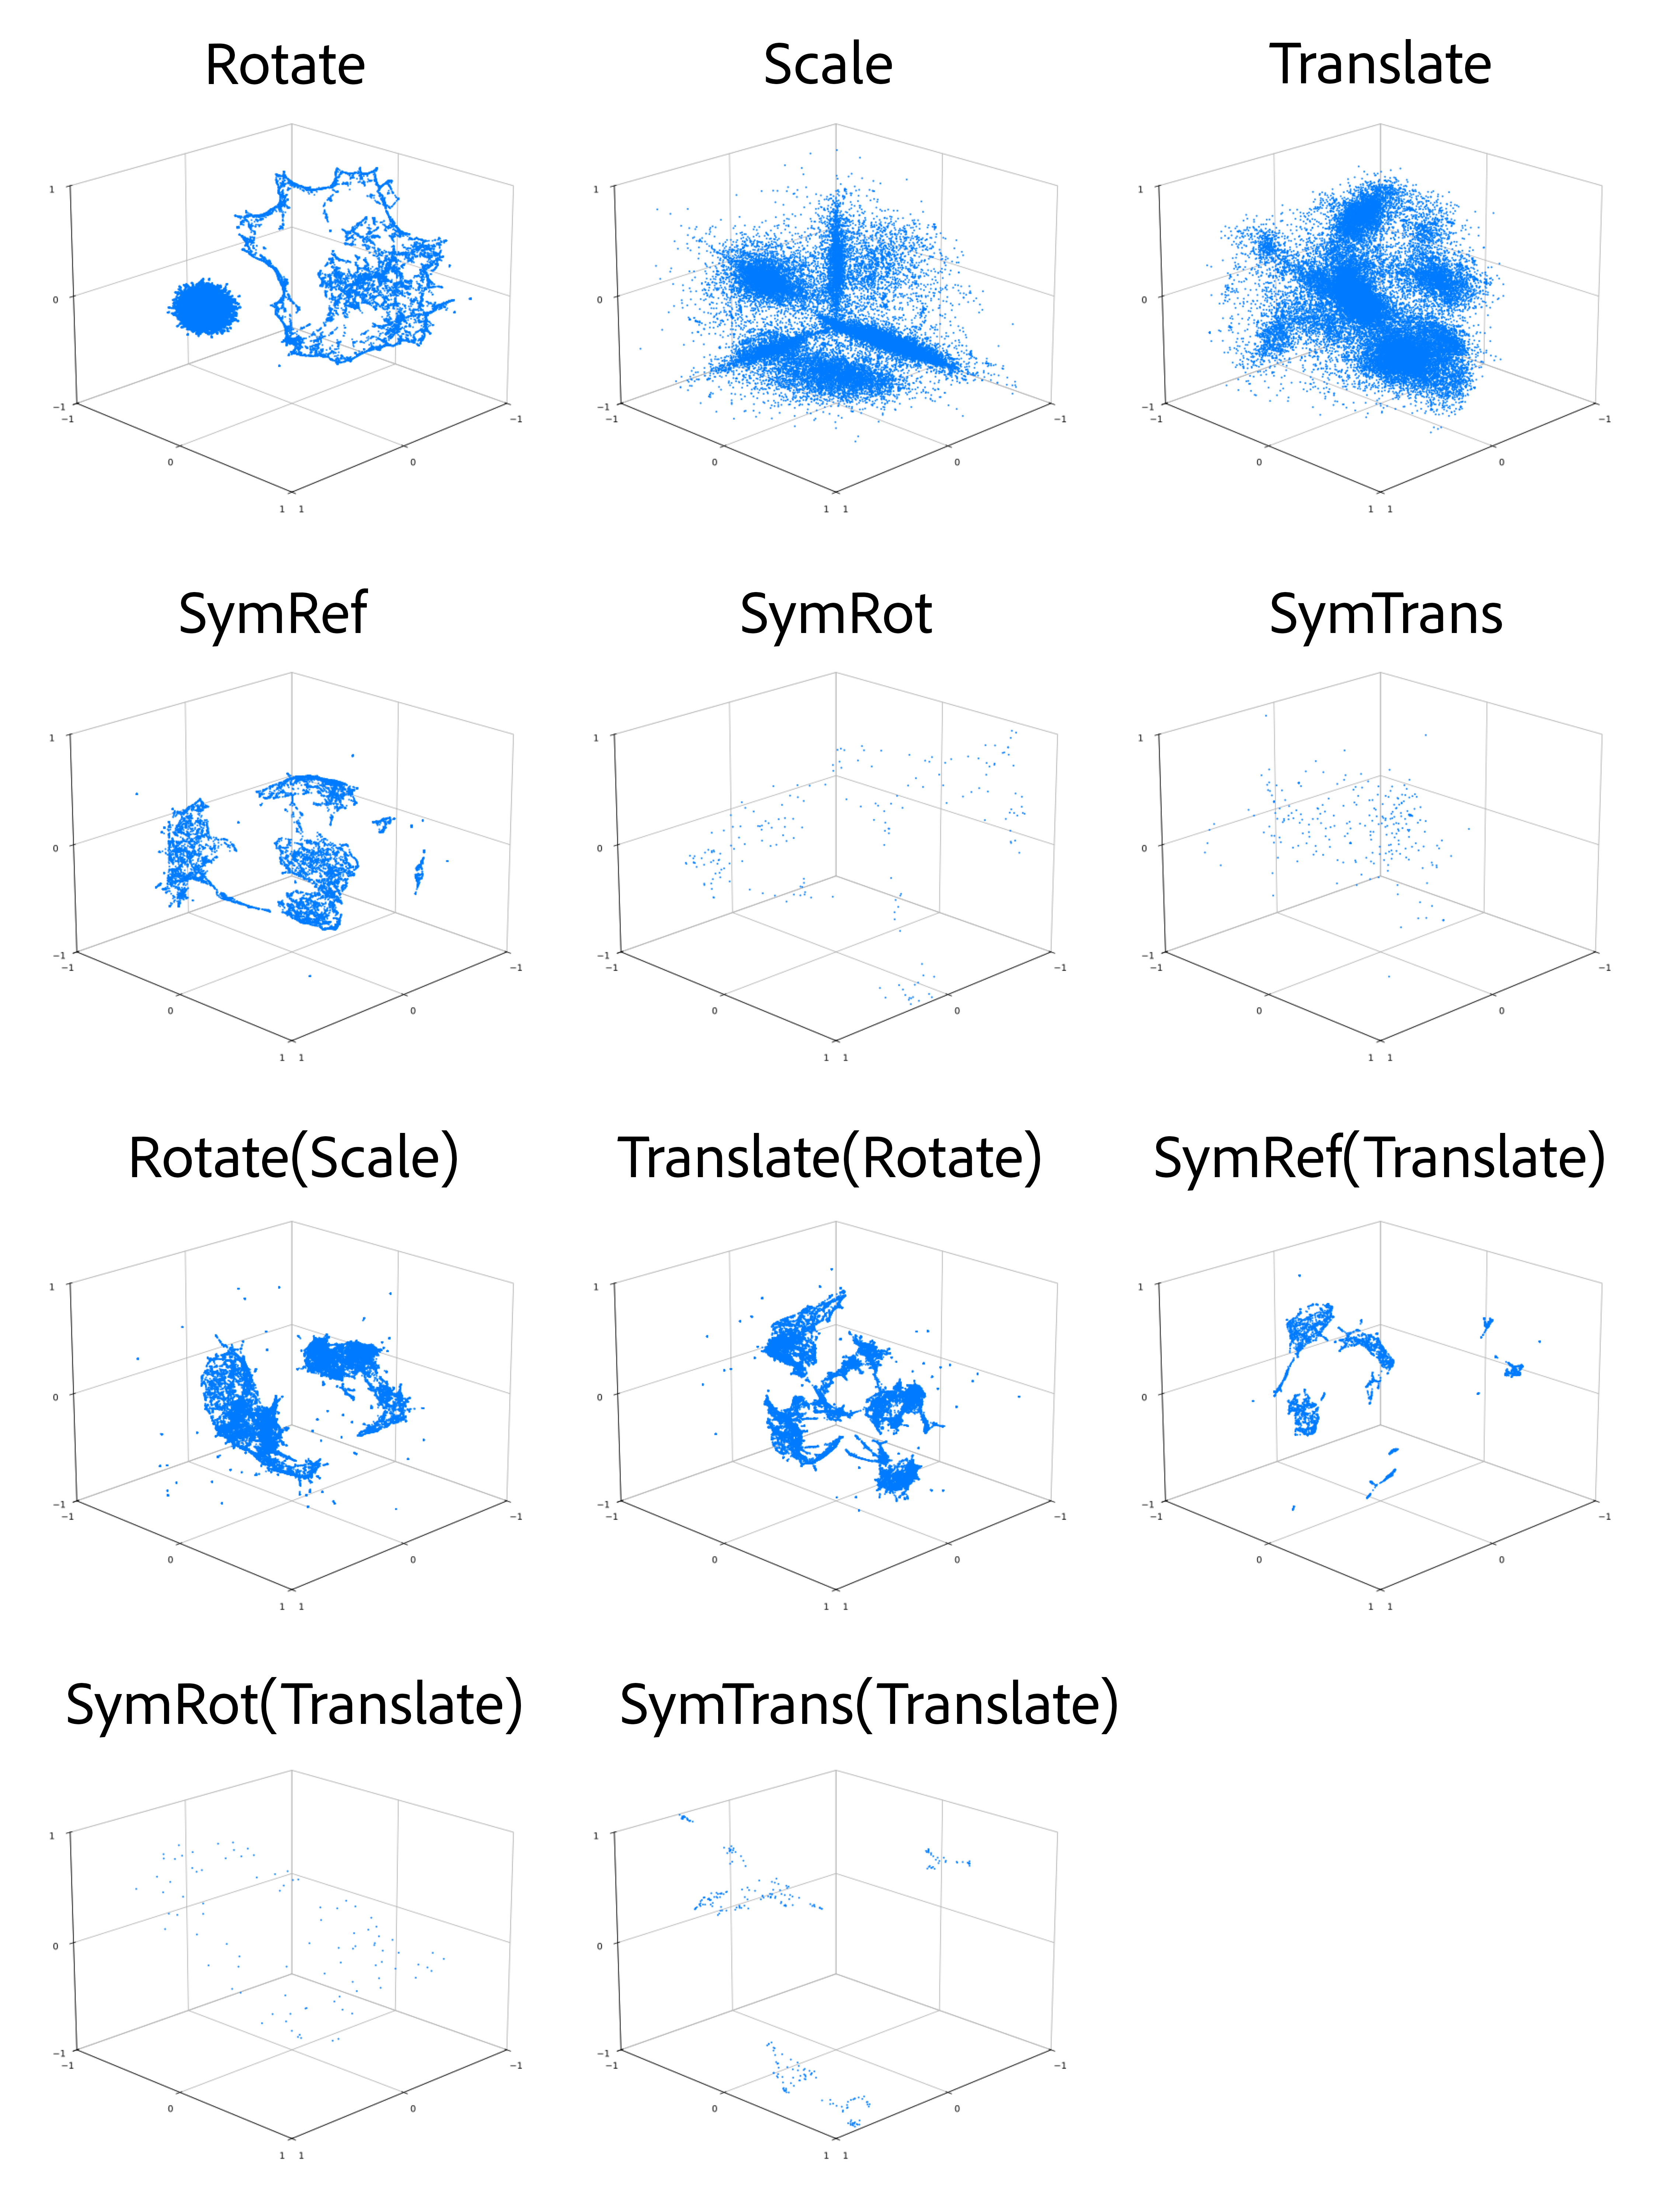
\includegraphics[width=\textwidth]{figures/structure_extraction.png}
    \caption{Visualizing the structure extraction process, where shape programs are decomposed into their constituent parametric relational units. For visualization, we use UMAP to reduce high-dimensional parameter spaces ($k > 3$) to 3D.}
    \label{fig:structure_extraction}
\end{figure}



% \section{Clustering and Dimensionality Analysis}

\section{Clustering Methodologies}
As illustrated in Figure \ref{fig:structure_extraction}, the extracted parameter spaces can be structured, with prominent clusters appearing around specific axes (e.g., in the scale space of primitive dimensions). Our next goal is to formally identify these clusters, representing stable subsets of recurring structures, that can be compressed into a lower-dimensional parametric manifold. To achieve this, we evaluate four clustering approaches to group the parameter spaces for each structural signature.

\subsection{Kmeans}

K-Means is a partitioning algorithm designed to organize a dataset $\mathbf{X}$ into $K$ mutually exclusive clusters by minimizing the variance within each group. In the context of 3D shape programs, it is utilized to identify high-density regions in the parameter space $\Theta$ that correspond to canonical part configurations. By assigning each primitive instance to its nearest centroid $\mu_k$, the algorithm provides a structured initialization for library discovery, effectively transforming a cloud of unstructured geometric attributes into a discrete set of structural types. 

The algorithm operates as an iterative expectation-maximization (EM) procedure that seeks to minimize the Within-Cluster Sum of Squares (WCSS), formally defined by the objective function:
\begin{equation}
    \mathcal{J}(\mathbf{M}, \mathbf{S}) = \sum_{k=1}^{K} \sum_{i=1}^{n} s_{ik} \| \mathbf{x}_i - \mu_k \|^2
\end{equation}
where $\mathbf{x}_i \in \mathbb{R}^d$ represents the $i$-th parameter vector in a dataset of $n$ samples, and $\mu_k$ is the centroid of the $k$-th cluster. The indicator variable $s_{ik} \in \{0, 1\}$ denotes whether point $i$ is assigned to cluster $k$, subject to the constraint $\sum_{k=1}^K s_{ik} = 1$. The matrices $\mathbf{M}$ and $\mathbf{S}$ represent the collective sets of all centroids and assignments, respectively. Optimization is achieved by alternating between two steps: first, updating assignments $\mathbf{S}$ by mapping each point $\mathbf{x}_i$ to its nearest centroid, and second, recomputing each centroid $\mu_k \in \mathbf{M}$ as the center of mass of its assigned points. The optimization works because it effectively performs a Voronoi tessellation of the parameter space.

Despite its efficiency, K-Means suffers from the Curse of Dimensionality and a fundamental spherical bias that renders it insufficient for complex shape datasets like PartNet. Another practical limitation is that K-Means requires the number of clusters $K$ to be chosen in advance. However, in discovery tasks, the number of naturally occurring geometric types is typically unknown. Furthermore, as the dimensionality $d$ of the parameter space increases, the ratio between the distance to the nearest and farthest neighbor tends toward zero, causing the $L_2$ norm to lose its discriminative power. When the algorithm attempts to slice these curved segments into convex Voronoi cells, it causes \textit{Data Distribution Fragmentation}.

While K-means provides a fast data partitioning, its hard boundaries and spherical assumption are often too restrictive for the overlapping stylistic variations in shape programs. This requires us to use a more flexible clustering model, leading us to Gaussian Mixture Models, which allow for non-spherical clusters and soft assignments.

\subsection{GMM}

To account for the uncertainty and overlapping stylistic traits in parameter distributions, we evaluate Gaussian Mixture Models (GMM) as a probabilistic framework for clustering. Unlike the previously discussed hard partitioning methods, GMM assumes that the parameter space $\mathbf{X}_{\mathcal{T}}$ is generated from a mixture of a finite number of Gaussian distributions with unknown parameters. We define the probability of a parameter vector $\mathbf{x}$ as:
\begin{equation}
    p(\mathbf{x}) = \sum_{k=1}^{K} \pi_k \mathcal{N}(\mathbf{x} | \mu_k, \Sigma_k)
\end{equation}
where $\mathbf{x} \in \mathbb{R}^d$ is the observed parameter vector, and $\mathcal{N}(\cdot)$ denotes a $d$-dimensional multivariate Gaussian distribution. For each component $k$, the parameters $\mu_k \in \mathbb{R}^d$ and $\Sigma_k \in \mathbb{R}^{d \times d}$ represent the mean vector and covariance matrix, respectively. The mixing weights $\pi_k$ define the relative contribution of each component to the global density, subject to the constraints $\pi_k \geq 0$ and $\sum_{k=1}^K \pi_k = 1$. This formulation allows for soft cluster assignments, represented by the posterior probability or ``responsibility'' of a component, reflecting the fuzzy semantic boundaries within the PartNet dataset.

The optimization of GMM parameters $(\pi, \mu, \Sigma)$ is performed via the Expectation-Maximization (EM) algorithm, which iteratively refines the posterior probability (responsibility) that each component $k$ generated point $\mathbf{x}_i$. A critical advantage of GMM over K-Means is the flexibility of the covariance matrix $\Sigma_k$. By allowing $\Sigma_k$ to be \textit{full} rather than \textit{spherical}, the model can capture ellipsoidal clusters oriented along any axis in the parameter space. This enables the algorithm to model linear correlations between part attributes, such as the proportional scaling of a table's width and depth.

Despite its probabilistic advantages, GMM is still fundamentally limited by a \textit{Linearity Constraint}. While it can model ellipsoidal clusters, it remains unable to approximate the complex, curved data distributions that our LID analysis identifies in Section~\ref{sec:lid_method}. Furthermore, in high-dimensional regimes, the number of parameters in the full covariance matrices grows quadratically, leading to numerical instability and the \textit{Singular Covariance} problem when data is sparse. 

We evaluate GMM not as a final solution for non-linear discovery, but as a robust way to represent abstractions without neural encoders. By projecting high-dimensional data onto the first $k$ eigenvectors of the covariance matrix $\Sigma_k$, essentially performing a cluster-specific Principal Component Analysis, we can create linear abstraction nodes. This GMM-based approach serves as a critical baseline, allowing us to evaluate whether a specific part category can be sufficiently explained by linear transformations or if it necessitates the more complex capacities of neural data distributions.

Although GMM allows for ellipsoidal clusters and probabilistic assignments, it remains less optimal for the assumption of a linear, Gaussian-based data distribution. To capture truly non-convex, manifold-like structures common in parametric data without assuming a specific parametric shape, we move toward density-based clustering.

\subsection{DBSCAN}

To overcome the geometric rigidity of centroid-based and linear probabilistic methods, we evaluate Density-Based Spatial Clustering of Applications with Noise (DBSCAN). Unlike K-Means or GMM, DBSCAN does not require a pre-specified number of clusters and identifies groups based on the local density of the parameter space $\Theta$. A point $\mathbf{x}$ is classified as a \textit{core point} if its $\epsilon$-neighborhood contains at least $minPts$ points, formally: $|N_\epsilon(\mathbf{x})| \geq minPts$, where $N_\epsilon(\mathbf{x}) = \{ \mathbf{y} \in \mathbf{X} \mid \|\mathbf{x} - \mathbf{y}\| \leq \epsilon \}$. This density-connectivity allows the algorithm to recover clusters of arbitrary, non-convex shapes.

The mathematical strength of DBSCAN lies in its ability to define clusters as maximal density-connected sets. A point $\mathbf{p}$ is density-reachable from $\mathbf{q}$ if there is a chain of core points leading from one to the other. This formulation provides a rigorous mechanism for noise suppression, as any point that is not density-reachable from a core point is labeled as an outlier. In the PartNet domain, this is particularly valuable for filtering topological anomalies, shapes with malformed primitives or unique geometries that do not belong to a consistent data distribution.

However, DBSCAN encounters a critical density collapse when applied to high-dimensional PartNet parameters. The algorithm relies on a global $\epsilon$ parameter, which assumes that the density required to define a part is uniform across the entire dataset. In 3D shape programs, this is rarely true, for instance, the parameter density for chair legs is often higher than the sparse distribution of backrests. Consequently, a single $\epsilon$ often fails to capture clusters of varying densities simultaneously, either merging distinct data distributions into a single blob or fracturing sparse clusters into noise.

DBSCAN provides the geometric flexibility needed for curved manifolds, yet its reliance on a global density threshold causes it to collapse when a dataset contains clusters of varying densities. This final limitation is resolved by Hierarchical DBSCAN, which replaces the global $\epsilon$ with a multi-scale reachability hierarchy.

\subsection{HDBSCAN}

To address the multi-density nature of the PartNet parameter space, we also use Hierarchical DBSCAN (HDBSCAN). This methodology extends density-based clustering by converting DBSCAN into a hierarchical clustering algorithm. The core advantage of HDBSCAN is the elimination of the global $\epsilon$ parameter, replaced by the \textit{mutual reachability distance} $d_{mreab}(a, b)$, defined as:
\begin{equation}
    d_{mreab}(a, b) = \max \{ core_k(a), core_k(b), d(a, b) \}
\end{equation}
where $core_k(x)$ is the distance to the $k$-th nearest neighbor. By building a minimum spanning tree based on this metric, HDBSCAN constructs a hierarchy of potential clusters (a dendrogram), allowing the system to simultaneously identify dense data distributions and sparse data distributions that earlier methods would fragment.

The mathematical selection of clusters from the hierarchy is governed by the principle of \textit{Persistence}. While HDBSCAN eliminates the need to pre-specify a single global $\epsilon$, it utilizes the concept of \textit{density} $\lambda = 1/\epsilon$ to evaluate the hierarchy. For each cluster $C$, we define $\lambda_{birth}(C)$ as the density level at which the cluster first merges into existence in the dendrogram. For each point $x$ within that cluster, let $\lambda_{death}(x, C)$ be the density value at which $x$ either falls out of the cluster (becoming noise) or the cluster splits. The \textit{stability} of a cluster $\sigma(C)$ is then calculated by summing the total persistence of all its members:
\begin{equation}
    \sigma(C) = \sum_{x \in C} (\lambda_{death}(x, C) - \lambda_{birth}(C))
\end{equation}
By maximizing this stability over the hierarchy, the algorithm automatically identifies the most persistent and robust data distributions without requiring the user to guess a single global density threshold. Furthermore, we utilize the Global-Local Outlier Score from Hierarchies (GLOSH) to identify noise. This is superior for 3D shape programs as it distinguishes between global noise and local stylistic outliers within a specific part category.

The transition to HDBSCAN is the final prerequisite for successful data distribution learning. In high-dimensional shape spaces, the ``true'' clusters often exist at varying scales of granularity. By utilizing the hierarchy and stability-based extraction, we ensure that our discovered abstractions represent the most stable structural units found in the dataset. Consequently, HDBSCAN emerges as the most robust methodology for high-dimensional shape programs, providing the ``clean'' and persistent geometric clusters required to transform unstructured primitives into the low-dimensional latent axes explored in the following sections.

\section{Local Intrinsic Dimensionality (LID) Estimation}
\label{sec:lid_method}

The primary objective of this phase is to determine the optimal latent bottleneck size $d_z$ for our neural macros. By measuring the irreducible degrees of freedom within each HDBSCAN cluster, we ensure that the downstream Autoencoder is geometrically consistent with the data's intrinsic complexity. This principled discovery distinguishes between ``ambient noise'' (high-dimensional, low-variance fluctuations) and ``functional variation'' (low-dimensional, high-variance geometric features), preventing the network from memorizing redundant fluctuations.

The process begins with a parameter cluster $\mathcal{C} \subset \mathbb{R}^k$ identified in the preceding stage, where $k$ is the ambient dimension. For every point $\mathbf{x}_i \in \mathcal{C}$ (where $n = |\mathcal{C}|$), we construct a local neighborhood $\mathcal{N}_K(\mathbf{x}_i)$ containing its $K$ nearest neighbors. We utilize a neighborhood size $K=30$ to maintain local manifold linearity while ensuring statistical stability against small-sample variance.

To achieve robustness against both non-linear curvature and varying cluster densities, we evaluate the local dimensionality through two complementary perspectives:

\textbf{Local PCA:} This method identifies the dimensionality of the local linear subspace at each point. For each point $\mathbf{x}_i$, we utilize its neighborhood $\mathcal{N}_K(\mathbf{x}_i)$ to compute a local covariance matrix $\mathbf{\Sigma}_i$. By analyzing the decay of the local ordered eigenvalues $\lambda_{i,1} \ge \dots \ge \lambda_{i,k}$, we derive a \textit{per-point spectral estimate} $d_{lpca, i}$ by locating the index $j \in \{1, \dots, k-1\}$ that maximizes the relative spectral gap:
    \begin{equation}
        d_{lpca, i} = \arg \max_{j} \left( \frac{\lambda_{i,j}}{\lambda_{i,j+1}} \right), \text{ subject to } \lambda_{i,j} > \alpha \lambda_{i,1}
    \end{equation}
    where $\alpha$ serves as a relative sensitivity threshold to filter out components indistinguishable from the ambient noise floor.

\textbf{TWO-NN:} This method provides a robust \textit{cluster-wide statistical estimate} for the entire dataset $\mathcal{C}$. We analyze the distance ratio $\mu = r_2/r_1$, where $r_1$ and $r_2$ represent the distances to the first and second nearest neighbors for each point. We solve for a single statistical dimension $d_{twonn}$ by linearizing the cumulative distribution function $F(\mu) = 1 - \mu^{-d_{twonn}}$ through a global least-squares fit:
    \begin{equation}
        -\ln(1 - \hat{F}(\mu)) = d_{twonn} \cdot \ln(\mu)
    \end{equation}
    where $\hat{F}(\mu)$ is the empirical CDF. This estimator remains robust to curvature by operating at the extreme local limit.

These two perspectives provide a robust estimation of the intrinsic dimensionality. Rather than serving as a direct derivation, these LID estimates provide a formal justification for the existence of a lower-dimensional manifold. By verifying that the points within a cluster share a consistent intrinsic dimensionality that is significantly lower than the ambient dimension $k$, we justify the application of a uniform bottleneck $d_z$ in the subsequent neural models.

This data-driven justification is critical for ensuring that the subsequent compression is \textit{topologically smooth}. By confirming the low-dimensional nature of the cluster parameters, we validate the transition to a compressed latent representation. Choosing $d_z$ based on this ``geometric sweet spot'' ensures the neural model has sufficient capacity to capture functional variation while remaining small enough to filter out stochastic ambient noise. The resulting dimension $d_z$ represents the irreducible description length of the part's parameters and serves as the direct architectural constraint for the \textit{Neural Abstraction Training} described in Section \ref{sec:neural_training}.

\section{Neural Abstraction Training}\label{sec:neural_training}

The second stage of our framework involves the synthesis of \textit{Neural Abstractions}. These modules function as learned macros that replace high-dimensional parametric variations with optimized latent encodings. Our framework implements three distinct compression backends of Principal Component Analysis (PCA), Autoencoders (AE), and Variational Autoencoders (VAE). This allows for a comparative analysis of \textit{expressive power} (linear vs. non-linear) and the \textit{interpretability and editability} of the resulting latent space, ensuring that the discovered abstractions are not only compact but also semantically meaningful.

\subsection{Linear Baseline: Principal Component Analysis (PCA)}

We utilize Principal Component Analysis (PCA) as a baseline for linear expressive power. PCA performs an orthogonal transformation to map the parameter matrix $\mathbf{X}$ into a coordinate system defined by the directions of maximal variance:
\begin{equation}
    \mathbf{Z} = (\mathbf{X} - \mu) \mathbf{W}_d
\end{equation}
where $\mu$ is the empirical mean and $\mathbf{W}_d$ contains the top $d$ eigenvectors derived from the covariance matrix. 

We use PCA as a linear baseline to benchmark the maximum representational accuracy achievable through purely linear methods. By establishing the minimum reconstruction error via standard orthogonal decomposition, PCA serves as a critical diagnostic for the data's complexity. This comparison allows us to quantify exactly when the data manifold becomes too complex for linear modeling, thereby justifying the transition to non-linear neural models for higher fidelity and better expressive power.

\subsection{Autoencoders (AE)}

While linear techniques like PCA provide a useful baseline, they are fundamentally limited to capturing variations along straight axes. In the context of PartNet, stylistic variations often reside on complex, non-linear structures. To capture these patterns, we utilize fully-connected Autoencoders. The theoretical motivation for this shift lies in the \textit{Universal Approximation Theorem}, which states that a neural network with at least two layers can approximate any continuous function on compact subsets of $\mathbb{R}^n$ to arbitrary precision, given sufficient width. This inherent expressive power allows the AE to utilize non-linear activation functions $\sigma(\cdot)$ to learn a deterministic mapping $f_\phi: \mathbb{R}^k \to \mathbb{R}^{d_z}$, effectively wrapping the latent space around the data's natural curvature. While the theorem provides an existential guarantee, it does not ensure that a suitable set of parameters can be easily discovered via optimization. However, it establishes the necessary capacity for our neural macros to identify patterns that linear models would perceive as high-variance noise.

The primary advantage of the AE in this pipeline is its ability to discover high-order correlations between parameters that do not scale proportionally. By optimizing the Mean Squared Error (MSE) between the input $\mathbf{x}$ and the reconstruction $\hat{\mathbf{x}} = g_\theta(f_\phi(\mathbf{x}))$:
\begin{equation}
    \mathcal{L}_{\text{AE}} = \mathbb{E}_{\mathbf{x} \sim \mathbf{X}} \left[ \| \mathbf{x} - g_\theta(f_\phi(\mathbf{x})) \|^2 \right]
\end{equation}
the model achieves a much lower reconstruction error on irregular parameter distributions. By learning to wrap the latent space around the natural curvature of the data, the AE provides a significant boost in representational accuracy over PCA, allowing it to capture high-order correlations that linear assumptions would miss.

\subsection{VAE with Lipschitz Continuity}


Traditional Autoencoders work by compressing input data into a single, deterministic point within a lower dimensional latent space. While effective for basic dimensionality reduction, this approach lacks a structural constraint on the latent manifold. In practice, this often results in a ``fractured'' latent space. Because the space between these points is largely \textit{meaningless}, any attempt to interpolate or navigate the latent space leads to geometric artifacts, i.e., outputs that do not represent valid or realistic geometries. Consequently, standard AEs are often unsuitable for tasks where smooth, interpretable transitions between shapes are required.

To overcome the sparsity of deterministic mappings, we implement a \textit{Variational Autoencoder (VAE)}. Unlike the standard AE, the VAE encoder maps inputs to a probability distribution, typically a Gaussian defined by a mean ($\mu$) and a variance ($\sigma$). By sampling from this distribution, $z \sim q_\phi(z|x)$, the model ensures that the latent space is locally dense. 

This works because of the inclusion of the \textit{Kullback-Leibler (KL) Divergence} term in the loss function, which forces the latent distributions to remain close to a standard normal distribution $\mathcal{N}(0, I)$. This regularization prevents the model from ``cheating'' by placing shapes far apart, effectively packing the latent space and ensuring that every region of the manifold corresponds to a meaningful geometric output.

While a VAE already addresses the problem of latent discontinuity, it does not inherently guarantee that the mapping is stable or intuitive for editing. A common issue even in probabilistic models is high sensitivity: a tiny perturbation in the latent vector $z$ can lead to a disproportionately large, discontinuous ``jump'' in the reconstructed geometry. To enhance the \textit{interpretability and editability} of our neural abstractions, we aim to enforce a relationship where small movements in latent space correspond to proportional changes in geometry. Specifically, we want to ensure that if a user moves one unit in the latent space, the decoded parameter vector also only changes by approximately one unit.

To enforce this smoothness, we require the network to be \textit{Lipschitz continuous}. A function $h(z)$ is $K$-Lipschitz if the ratio of the change in output to the change in input is bounded by a constant $K$: $\|h(z_1) - h(z_2)\| \leq K \|z_1 - z_2\|$. By targeting $K \approx 1$, we ensure that the ``speed'' at which the geometry changes relative to latent coordinates remains stable. We achieve this by combining a \textit{hard architectural constraint} with a \textit{soft regularization penalty}:

\textbf{Spectral Normalization (Hard Constraint):} We normalize the weight matrices $W$ of each layer by their largest singular value (the spectral norm $\sigma(W)$), such that $\hat{W} = W / \sigma(W)$. This ensures that each layer is 1-Lipschitz, thereby bounding the global Lipschitz constant of the entire network to be $\leq 1$. This prevents gradient explosions and ensures the network is globally stable across the entire manifold.

\textbf{Lipschitz Penalty (Soft Regularizer):} To further refine the local mapping and ensure the latent space is not just bounded but also intuitive, we add an explicit Lipschitz loss, $\mathcal{L}_{\text{Lip}}$. This term penalizes cases where the local gradient deviates from unity, encouraging a ``one-to-one'' relationship between latent movement and parameter change. 

To integrate these requirements, we define a multi-objective loss function. We supplement the standard reconstruction loss ($\mathcal{L}_{\text{rec}}$) and the KL Divergence with the Lipschitz regularization term:
\begin{equation}
\mathcal{L}_{\text{Lip}} = \mathbb{E}_{z_1, z_2} \left[ \left| 1 - \frac{\|h(z_1) - h(z_2)\|}{\|z_1 - z_2\|} \right| \right]
\end{equation}

The final total loss used to train the network is defined as:
\begin{equation}
\mathcal{L}_{\text{total}} = \mathcal{L}_{\text{rec}} + \beta D_{\text{KL}}(q_\phi(z|x) \| \mathcal{N}(0, I)) + \gamma \mathcal{L}_{\text{Lip}}
\end{equation}
where $\beta$ controls the density of the latent space and $\gamma$ governs the smoothness of the geometric transitions.

Our implementation of Lipschitz continuity and spectral normalization in the VAE architecture is inspired by the work on certifiably robust Variational Autoencoders by Barrett et al. \cite{Barrett2021}, utilizing their open-source codebase \cite{Barrett_Lipschitz_VAEs}.

\subsection{Iterative Refinement and Outlier Filtering}

A challenge to be noted in training on datasets like PartNet is the presence of geometric outliers, i.e. instances that, while sharing a structural signature, possess parameter distributions that deviate wildly from the cluster's manifold. These outliers often arise from non-standard modeling practices, topological noise, or instances that effectively belong to a different geometric cluster, or no consistent cluster at all. Crucially, the objective of our discovery process is not to abstract every part of every chair; rather, we aim to discover and model only those components where we are actually confident that they are the result of an interesting, recurring pattern. To address this, our implementation utilizes a multi-pass \textit{iterative retraining loop} designed to prune the dataset of instances that the model cannot efficiently represent. This refinement increases the reliability of the abstraction by focusing the model's capacity on the most stable and statistically significant structural regularities.

The process begins with an initial fit and manifold discovery phase, where the chosen model is trained on the full set of normalized parameters $\mathcal{P}$ for a given cluster. This initial pass serves as a coarse grained discovery phase. Following, we perform reconstruction error profiling where we calculate the Max Absolute Error (MAE) for every instance $p \in \mathcal{P}$ in the normalized space, defined as $E(p) = \| \hat{p} - p \|_{\infty}$, where $\hat{p}$ is the reconstructed parameter vector. Instances exceeding a normalized threshold $\epsilon_{\tau}$, typically set at $0.05$, are flagged as outliers. This threshold represents a strict tolerance for how much a specific part can vary from its structural neighbours before it is considered a non-standard instance that would degrade the quality of the learned abstraction.

In the final stage of the loop, the dataset is masked to include only these ``well-explained'' instances, creating a refined subset $\mathcal{P}_{refined}$ upon which the model is retrained. By removing the influence of outliers, the latent axes are able to align precisely with the most stable modes of variation within the data. This iterative sub-sampling and retraining ensures that the resulting \textit{Abstraction} nodes represent a high-fidelity version of the pattern rather than a noisy average. This cycle may be executed for multiple iterations ($N_{retrain}$) until desired convergence is reached.

\subsection{Geometric Fidelity and Verification}

While the iterative filtering protocol ensures parametric consistency, numerical proximity in a model's latent space does not always guarantee geometric fidelity. A primary challenge in neurosymbolic discovery is that tiny errors in specific parameters (e.g., a rotation quaternion) can lead to disproportionately large displacements in the resulting 3D point cloud. Furthermore, numerical stability does not inherently guarantee that the \textit{configurational topology}, the relative spatial arrangement and connectivity of parts is maintained after the abstraction is expanded. To address this, we implement a final geometric fidelity check to validate the transition from latent variables back to physical forms.

To perform this check, we generate 3D point clouds for both the original symbolic program and its neural reconstruction. This is achieved by recursively expanding the DSL hierarchy down to its primitive \texttt{Box} components and sampling points uniformly across their surfaces and volumes. We then evaluate the \textbf{Symmetric Chamfer Distance} to measure the spatial alignment between these two point clouds, $X$ and $Y$:
\begin{equation}
    \mathcal{D}_{Chamfer}(X, Y) = \frac{1}{|X|} \sum_{x \in X} \min_{y \in Y} \|x - y\|^2 + \frac{1}{|Y|} \sum_{y \in Y} \min_{x \in X} \|x - y\|^2
\end{equation}
This metric provides a robust measure of how closely the reconstructed shape matches the original. By enforcing a strict geometric threshold $\epsilon_{geo}$ (e.g., $0.05$ units), we ensure that the neural macro has correctly learned the underlying topology and spatial extent of the part assembly. If the expanded abstraction produces a point cloud that deviates from the original, it indicates a failure to preserve the structural integrity of the shape program, and the abstraction is rejected. This dual validation approach serves as a rigorous guarantee that every entry in the final library is both statistically stable and geometrically faithful to the original design intent.

%%% EGRAPHS

\section{E-Graph Integration and Equality Saturation}

Once a neural abstraction is identified and validated, it must be integrated back into the original shape programs. However, determining where to place these abstractions, and verifying that they truly lead to a lower global description length is a complex combinatorial problem. To address this, we implement a global structural refactoring phase inspired by the \textit{refactor} operation in ShapeCoder \cite{ShapeCoder}. We utilize the \texttt{egglog} E-graph engine \cite{Willsey2021} to act as a ``logical reasoning layer'', exploring the version space of equivalent programs to identify the optimal configuration of abstractions and symbolic operators.

\subsection{Non-Greedy Refactoring via E-Graphs}

The primary advantage of using an E-graph is the avoidance of a greedy integration strategy. In typical greedy systems, an abstraction is applied at the first matching location, potentially blocking a more significant optimization elsewhere in the program tree. By contrast, the E-graph allows the original ``flat'' geometry and all possible abstracted versions to coexist and compete within a unified data structure. We bridge the gap between our neural discovery environment and the logic engine through a four-stage process:
\begin{enumerate}
    \item \textbf{Lifting:} The program is serialized into a symbolic expression where parameters and operators are represented as e-nodes.
    \item \textbf{Saturation:} The engine applies a set of algebraic and library-specific rules to discover equivalent representations, such as merging nested offsets or replacing sub-trees with neural abstractions.
    \item \textbf{Extraction:} Using the weighted cost model in Table \ref{tab:egg_costs}, the engine identifies the single representation within the version space that achieves the global minimum cost.
    \item \textbf{Lowering:} The optimized symbolic string is reconstructed into a functional shape program, integrating the newly placed \textit{Abstraction} nodes.
\end{enumerate}

\subsection{Semantic Rewrite Rules}

To navigate the version space effectively, the E-graph utilizes a ruleset $\mathcal{R}$ that defines the algebraic identities of the shape DSL. In the following rules, we let $T$ and $R$ denote transformation operators, $\theta$ represent their associated continuous parameters, and $Abs(\cdot)$ signify a neural abstraction node. The symbol $+$ is used as shorthand for the $Union$ operator, while lowercase letters ($s, c, x, y, \dots$) serve as placeholders for sub-trees or shape expressions. These rules fall into several primary categories:

\begin{itemize}
    \item \textbf{Structural Identities} ($T(T(s, \theta_1), \theta_2) \to T(s, \theta_1 + \theta_2)$): Simplifies the tree by merging nested transformations or removing identity no-ops (e.g., $Scale(1,1,1)$).
    \item \textbf{Expansion Rules} ($T(Abs(c), \theta) \to Abs(T(c, \theta))$): Enables global optimization by allowing transformations to propagate ``through'' neural abstractions to common children.
    \item \textbf{Distributive Laws} ($T(x, \theta) + T(y, \theta) \to T(x + y, \theta)$): Pulls shared transformations out of $Union$ nodes to reveal deeper structural identities. Also applies to $Rotate$ and $Scale$.
    \item \textbf{Algebraic Identities} ($a + (b + c) \to (a + b) + c$): Enforces commutativity ($a+b \to b+a$) and associativity of the $Union$ operator to explore alternative tree topologies.
    \item \textbf{Commutativity of Ops} ($T(R(s, q), t) \to R(T(s, t), q)$): Allows the engine to reorder transformations (e.g., Translate and Rotate) to reveal matching structural patterns.
    \item \textbf{Symmetry Folding} ($T(s, \theta) + T(s, -\theta) \to SymRef(s, \text{plane})$): Identifies mirrored or repeated structural branches and collapses them into compact symmetry operators.
\end{itemize}

A critical challenge arises from the fact that neural abstractions can act as ``logical barriers'' that hide the underlying geometry from the engine. For example, if a chair leg is abstracted into a VAE node, the E-graph can no longer ``see'' the individual boxes inside to determine if they could be factored with external parts. We resolve this by implementing Expansion Rules (e.g., \textit{Transparency}) that allow transformations to propagate ``through'' an abstraction. This enables the engine to uncover global structural regularities (like category-wide symmetries) that would otherwise remain isolated within the local macro.

\subsection{Weighted Cost Modeling}

To navigate the trade-off between structural simplicity and parametric compression, we implement a \textbf{weighted cost model} within the E-graph. In this schema, weights are assigned to each DSL operator to guide the \texttt{egglog} engine toward the most efficient representation (Table \ref{tab:egg_costs}). We assign a minimal weight to the \texttt{Union} operator to encourage the formation of hierarchical groupings, while neural \texttt{Abstraction} nodes are assigned a weight lower than individual primitives to favor neural compression over raw primitive lists. Note that while these weights guide per-program extraction, the global library overhead is managed during the integration phase by penalizing the total number of unique abstractions in the DSL.

\begin{table}[htbp]
\centering
\caption{Egglog Cost Schema for Shape Program Operators.}
\label{tab:egg_costs}
\renewcommand{\arraystretch}{1.2}
\begin{tabular}{@{}lc p{0.55\textwidth}@{}}
\toprule
\textbf{Operator} & \textbf{Weight} & \textbf{Explanation} \\ \midrule
\texttt{Union} & 0.5 & Encourages early consolidation of parts into semantic groups. \\
\texttt{Abstraction} & 0.8 & Incentivizes neural compression over raw primitive parameter lists. \\
\texttt{Box}, \texttt{Cuboid} & 1.0 & Base weight for fundamental geometric building blocks. \\
\texttt{Transforms} & 1.1--1.3 & Standard $T, R, S$ operators; ranges reflect parameter complexity (e.g., $R$ vs $T$). \\
\texttt{Symmetries} & 1.5--1.7 & Prioritizes discovering deep structural patterns over simple primitive repetition. \\
\bottomrule
\end{tabular}
\end{table}



%%%%%%%%%%%%%%%%%%%%%%%%%%%%%%%%%%%%%%%%%%%%%%%%%%%%%%%%%%%%%%%%%%%%%%%%%%%%%%%
% CHAPTER: EVALUATION
%%%%%%%%%%%%%%%%%%%%%%%%%%%%%%%%%%%%%%%%%%%%%%%%%%%%%%%%%%%%%%%%%%%%%%%%%%%%%%%

\chapter{Evaluation}\label{ch:evaluation}

\section{Datasets}

\subsection{PartNet-Symh}\label{eval_dataset}
To evaluate the effectiveness of our neural abstractions, we utilize the \textbf{PartNet-Symh} dataset \cite{Yu_2019_CVPR, Mo_2019_CVPR}, which augments the PartNet benchmark with a recursive hierarchical organization of fine-grained parts for each shape. This dataset represents 3D objects through a top-down recursive decomposition into their constituent parts, organized as a \textit{symmetry hierarchy} (see \autoref{fig:partnetsymhexample}).

The dataset contains 22,369 3D shapes across 24 categories (e.g., Chair, Table, Storage, Lamp). Each shape's hierarchy is composed of three types of nodes: \textit{Type 0 (Leaf nodes)} representing individual geometric segments, \textit{Type 1 (Adjacency nodes)} indicating the proximity and connectivity between adjacent parts, and \textit{Type 2 (Symmetry nodes)} representing either reflectional or rotational symmetry relations across multiple parts, storing the specific parameters of the symmetry transformation (e.g., reflection planes or rotation axes).

A key advantage of this dataset is that shapes within the same category share a consistent high-level structure. For example, all chair models are decomposed into a consistent set of major semantic parts like a back, seat, and legs at the top levels of their hierarchies. This structural consistency ensures that the neural modeling of parametric distributions can capture meaningful geometric variations while adhering to the shared logical structure of the object category.

\begin{figure}[htbp]
    \centering
    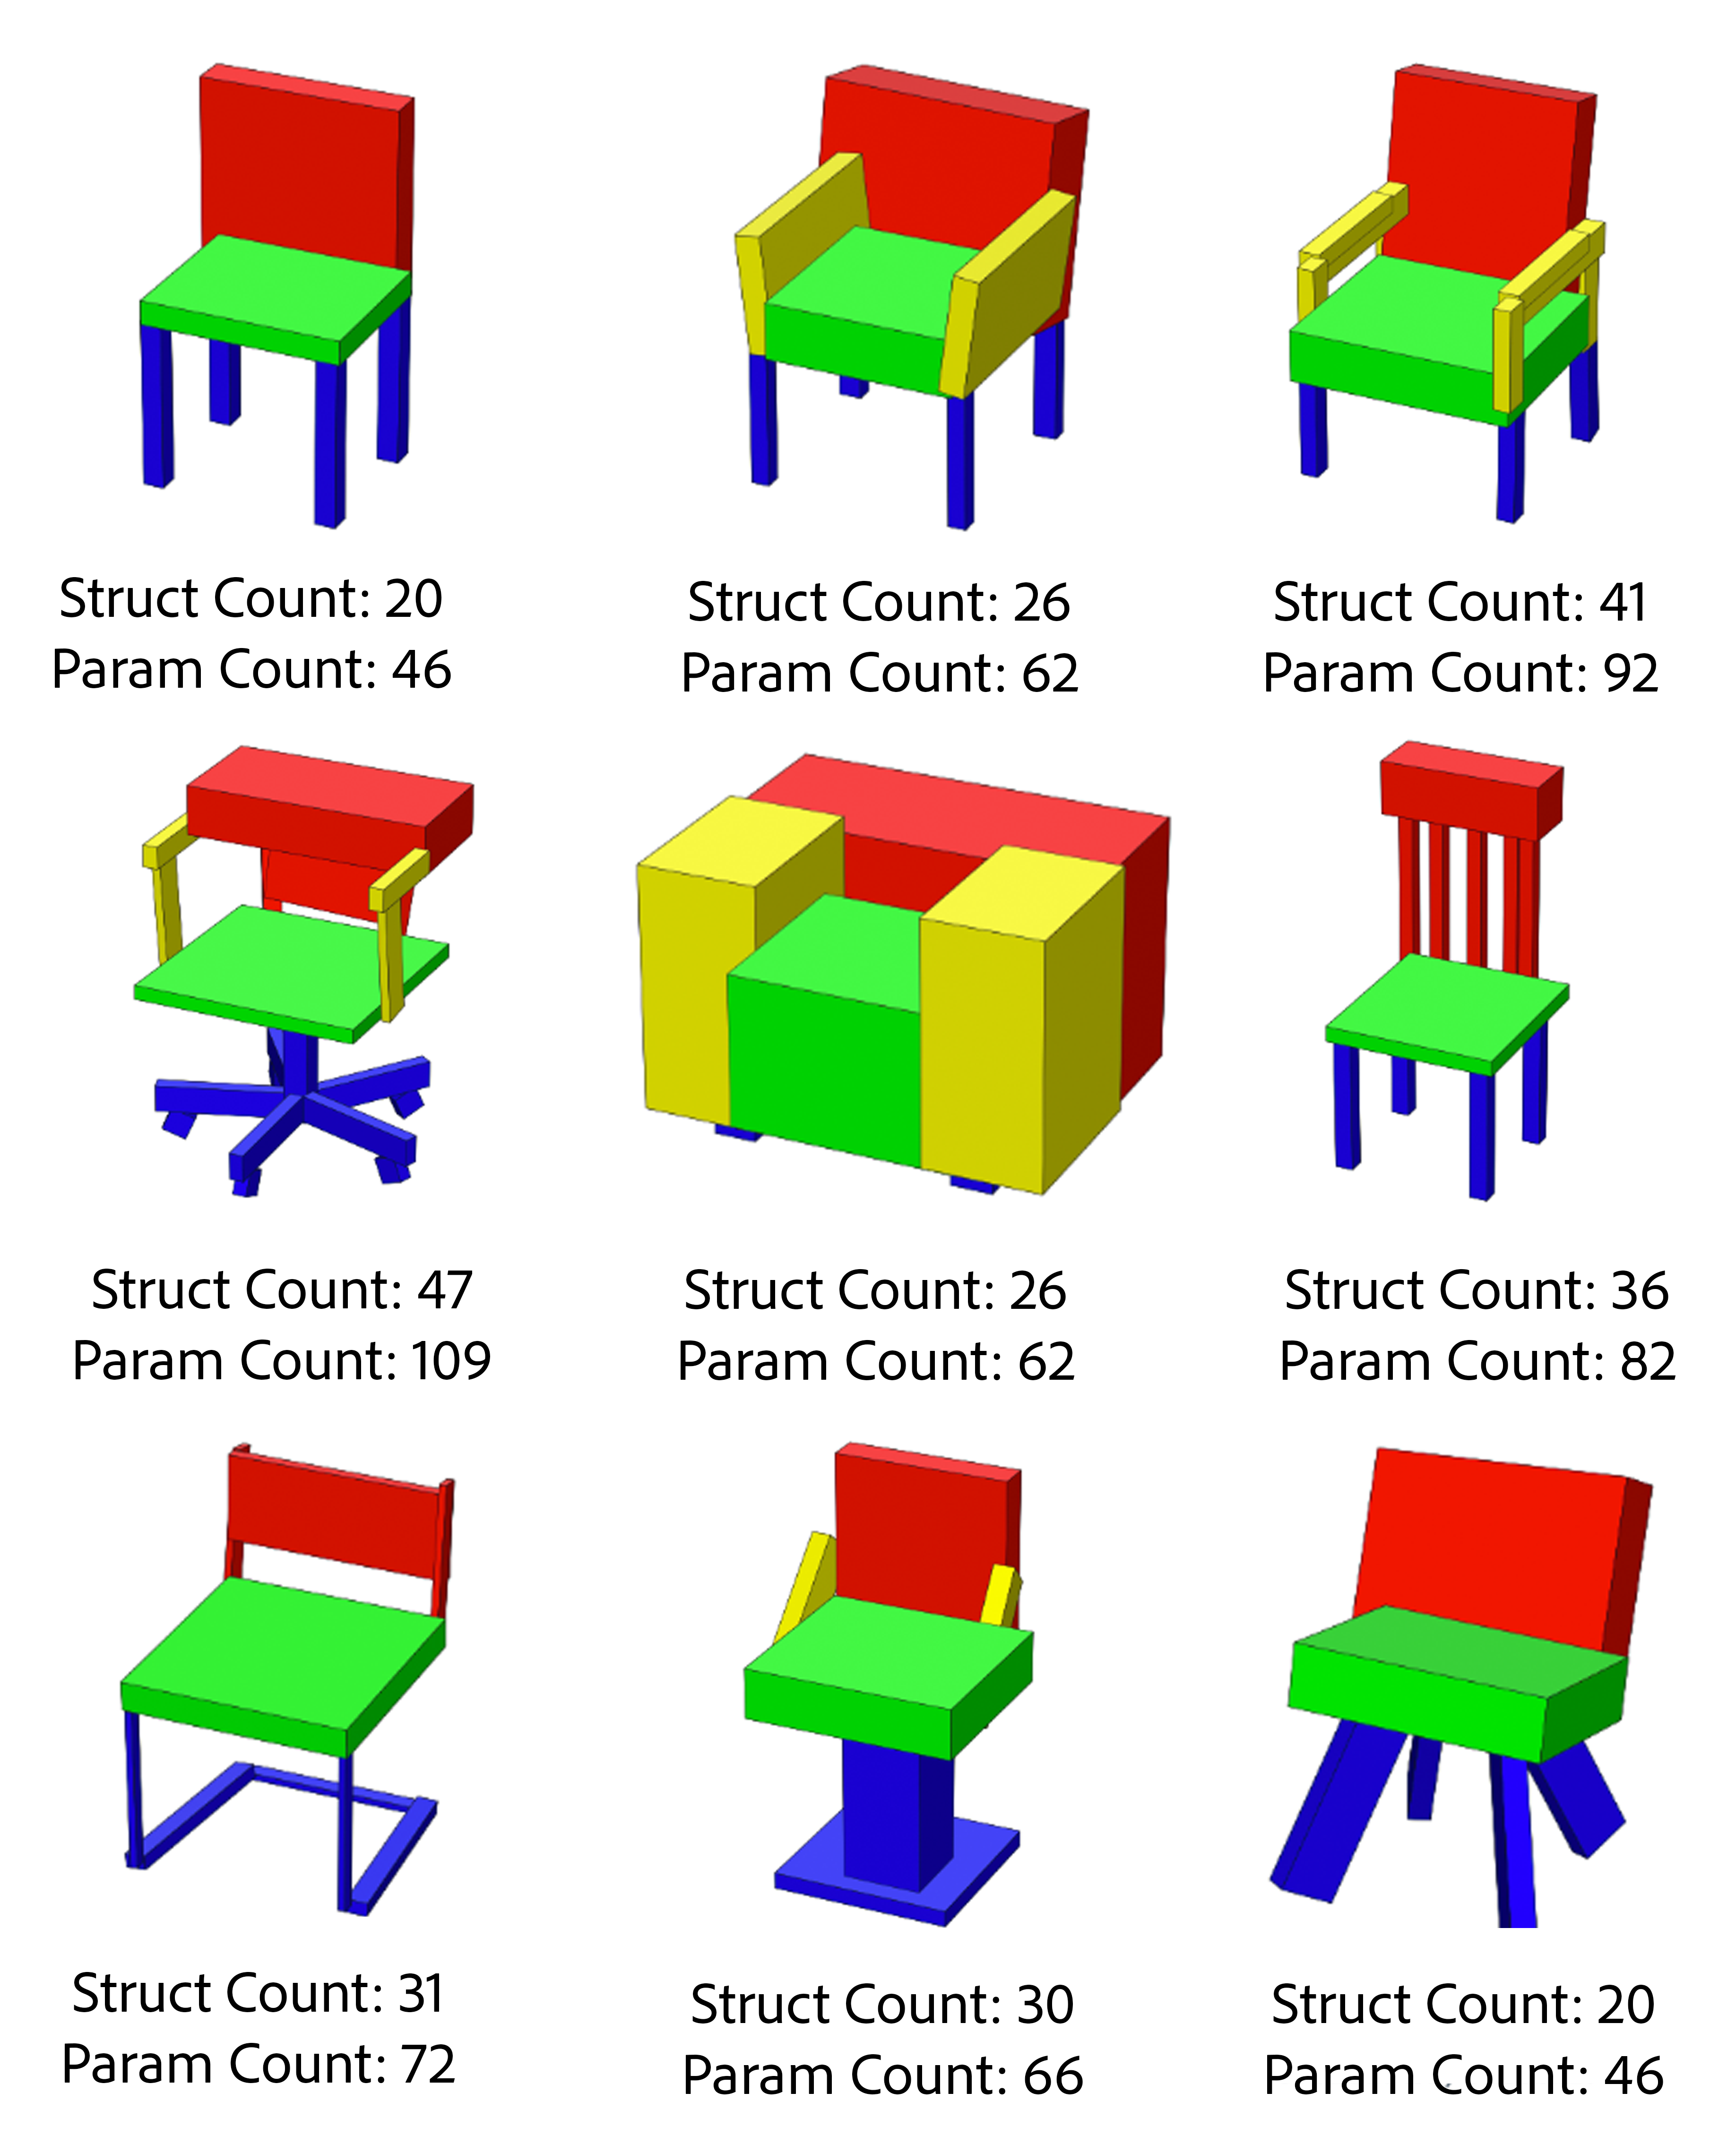
\includegraphics[width=0.95\textwidth]{figures/partnetsymhexample.png}
    \caption{Representative examples from the PartNet-Symh dataset. The figure illustrates the initial complexity of various 3D models in terms of their raw structure count and parameter count. Our primary goal is to discover abstractions that reduce these counts to achieve more compressed and manageable representations.}
    \label{fig:partnetsymhexample}
\end{figure}


\subsection{PartNet-ShapeCoder}
We also evaluate our method against the original \textit{PartNet-ShapeCoder} dataset to provide a direct comparison with rule discovery approaches. Crucially, while \textit{PartNet-Symh} preserves the raw, high-precision floating-point values from the original 3D geometry, the \textit{ShapeCoder} authors employ aggressive preprocessing to round these values and simplify the structural representation.

The base library in \textit{PartNet-ShapeCoder} is minimal, consisting primarily of \texttt{Union}, \texttt{Rotate}, \texttt{Translate}, and \texttt{Cuboid} operators. While \textit{PartNet-Symh} uses explicit symmetry nodes in its hierarchy, in \textit{PartNet-ShapeCoder} symmetry operations (\texttt{sym}) are incorporated into the rewrite rules rather than being hardcoded as base primitives. Furthermore, rotations in \textit{PartNet-ShapeCoder} are often restricted to fixed axes (e.g., \texttt{AX}, \texttt{AY}, \texttt{AZ}), which we convert into a numerical format to maintain consistency with our model architecture. This extensive preprocessing is designed to allow rule discovery engines to find exact patterns that would be obscured by raw geometric noise. We evaluate on \textit{PartNet-ShapeCoder} to provide a direct comparison with parameters optimized for symbolic solvers, and on \textit{PartNet-Symh} to demonstrate that our neural abstractions are robust to the high-precision data that frequently causes discrete symbolic solvers to fail.

\section{Clustering Analysis}\label{sec:clustering_analysis}

\begin{figure}[htbp]
    \centering
    \includegraphics[width=\textwidth]{figures/allcluster.png}
    \caption{Comparative analysis of clustering methodologies across various parametric signatures. Each row corresponds to a specific structural signature (Singleton or Pair), while each column evaluates a different clustering algorithm: K-Means, GMM, DBSCAN, and HDBSCAN. High-dimensional parameters are projected into 3D using UMAP for visualization purposes. Discrete colors indicate successfully identified clusters, while gray points denote samples classified as noise or outliers.}
    \label{fig:clustersv2}
\end{figure}

To identify stable structural clusters within the high-dimensional parameter space of PartNet signatures, we evaluate four distinct clustering methodologies. As illustrated in \autoref{fig:clustersv2}, the choice of algorithm significantly impacts the stability and quality of the resulting data distributions, which in turn determines the success of the subsequent neural abstraction training.

We observe that traditional centroid-based and linear probabilistic methods fail to capture the underlying geometry of the PartNet parameter space. \textit{K-Means} exhibits a strong spherical bias; this leads to \textit{data distribution fragmentation}, where a single continuous geometric manifold is erroneously fractured into multiple disjoint clusters. Similarly, while \textit{Gaussian Mixture Models (GMMs)} provide probabilistic ``soft'' assignments, they remain constrained by the assumption of Gaussian, ellipsoidal distributions, which poorly fits the complex, curved manifolds often found in shape programs.

In contrast, \textit{DBSCAN} demonstrates improved performance by identifying clusters as density-connected sets, allowing for the discovery of non-convex manifolds. However, its effectiveness is limited by the requirement of a global $\epsilon$ parameter. In the PartNet dataset, parameter densities vary significantly between part categories (e.g., the dense parameter space of legs versus the sparse distribution of decorative backrest slats). Consequently, this leads to ``linkage artifacts'' where distinct data distributions are merged or sparse but meaningful clusters are discarded as noise.

The most consistent and robust results are achieved using \textit{HDBSCAN}. By replacing the global $\epsilon$ with a multi-scale reachability hierarchy, HDBSCAN effectively handles the varying densities inherent in 3D shape programs. It successfully identifies persistent clusters across different levels of granularity without requiring manual tuning of the $\epsilon$ parameter. As demonstrated in our results, HDBSCAN provides the most stable foundation for neural training, ensuring that the induced abstractions correspond to genuine, high-density geometric regularities. This architectural decision proves to be very important; by isolating clean clusters from high-dimensional noise, we allow the subsequent Autoencoders to learn efficiently without being distracted by topological outliers.


\section{Local Dimensionality Analysis}\label{sec:lid_analysis}

\begin{figure}[htbp]
    \centering
    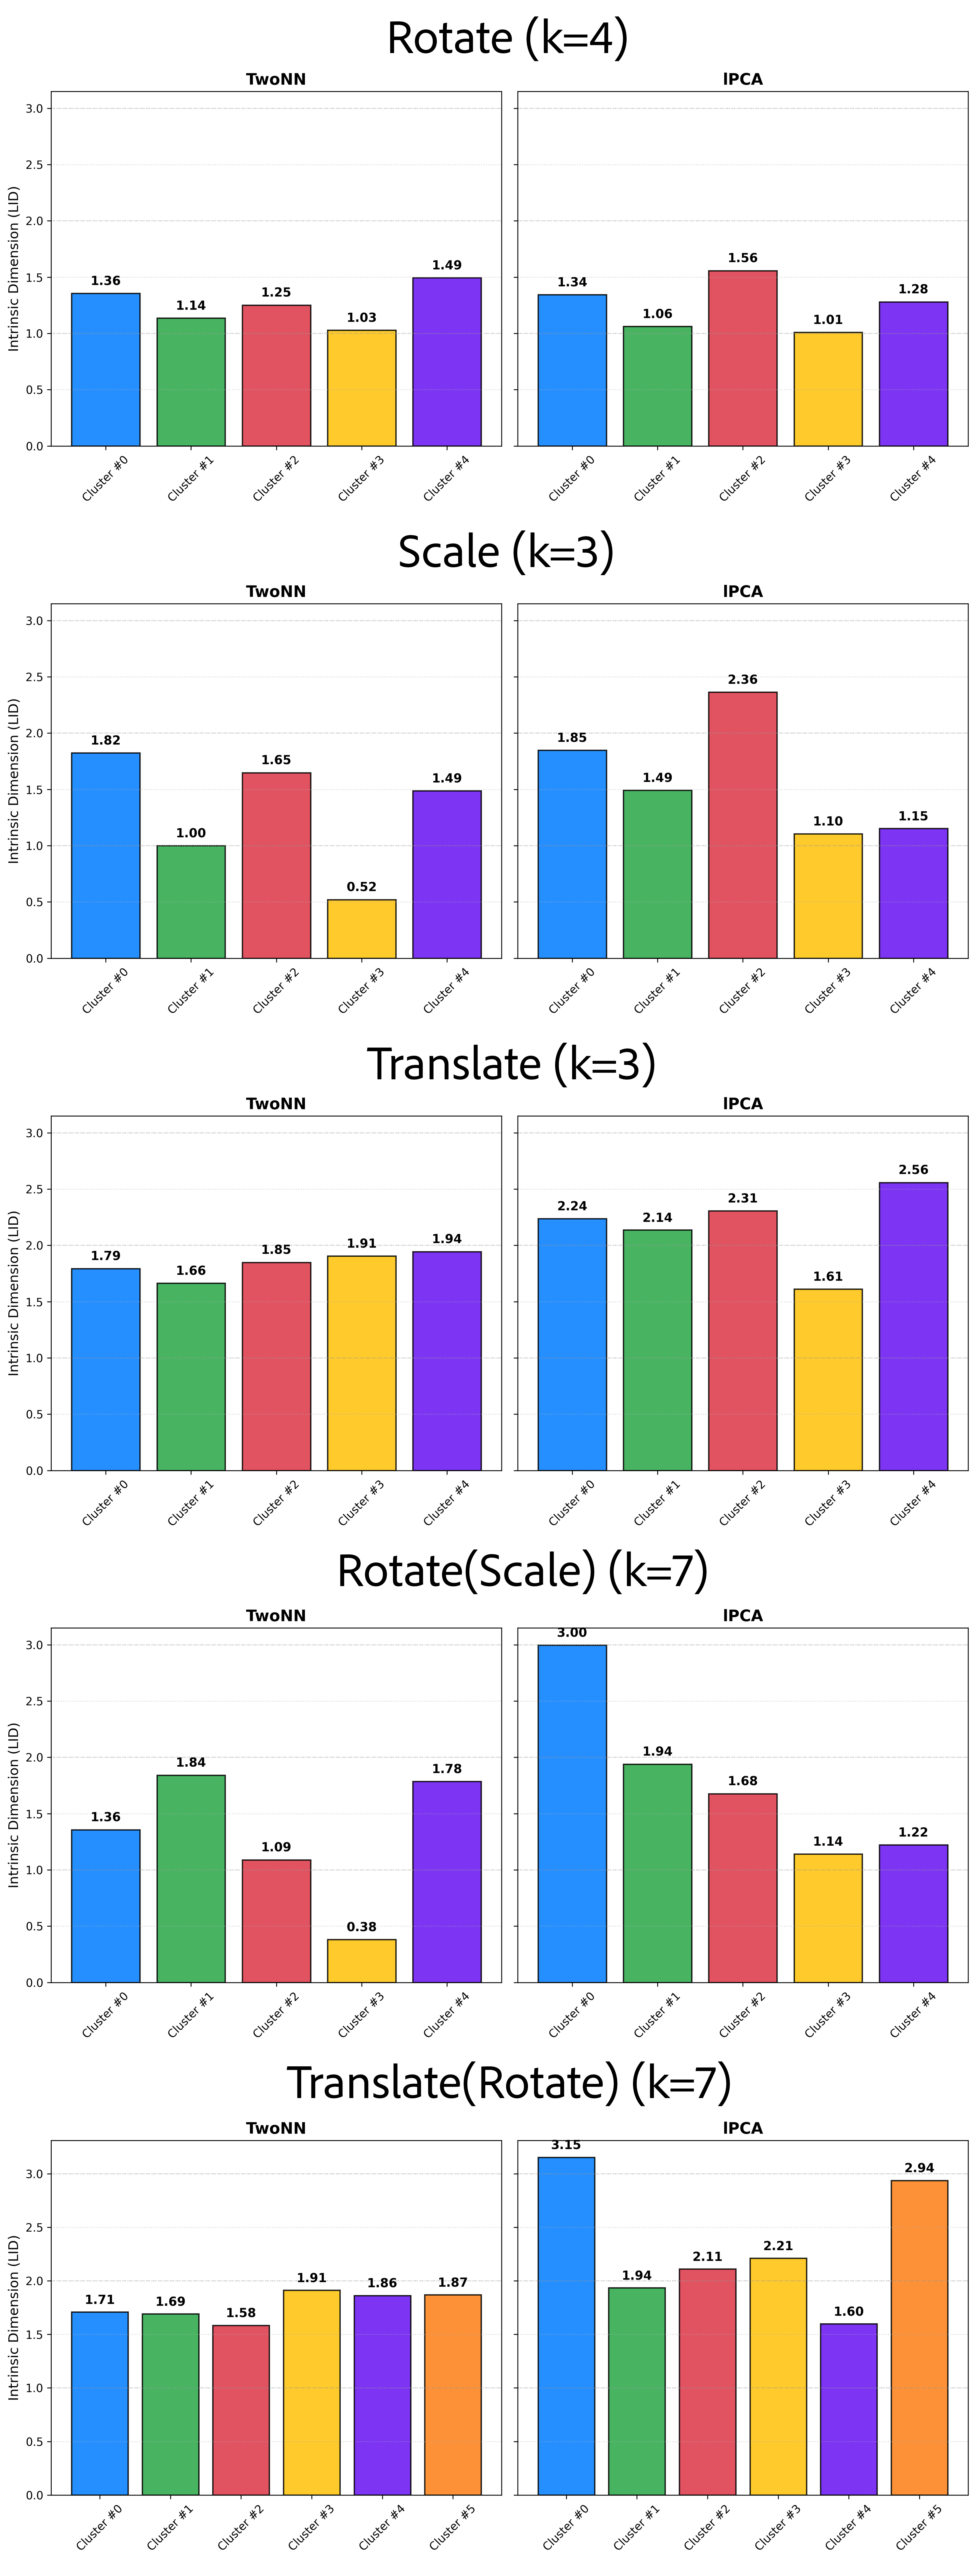
\includegraphics[width=0.5\textwidth]{figures/lidv2.png}
    \caption{Local Intrinsic Dimensionality (LID) estimation across stable HDBSCAN clusters for various structural signatures. Each row displays the estimated ID for a signature and its ambient dimension $k$, comparing results from the \textbf{Two-NN} and \textbf{Local PCA} estimators. The bar colors correspond to the clusters identified in Section \ref{sec:clustering_analysis} (see Figure \ref{fig:clustersv2}).}
    \label{fig:lid}
\end{figure}

To provide justification for our neural bottleneck selection, we perform a Local Intrinsic Dimensionality (LID) analysis on the stable clusters discovered via HDBSCAN. As illustrated in \autoref{fig:lid}, we observe a significant discrepancy between the original dimension of the raw primitive parameters and the intrinsic dimensionality of the underlying geometric manifold.

For the structural signatures, the ambient dimension $k$ ranges from 3 up to 12. However, our LID estimates, calculated using the \textbf{Two-NN} and \textbf{Local PCA} methods, consistently identify intrinsic dimensions between $d \approx 1$ and $d \approx 4$. We observe that \textbf{Two-NN} often yields lower estimates as it operates at the extreme local limit ($k=2$) and remains robust to the ``thickness'' of the manifold caused by noise, whereas \textbf{Local PCA} utilizes a larger neighborhood ($K=30$) that is more sensitive to curvature and stochastic variations. This reveals that a large percentage of the parameter variance in the PartNet dataset is redundant, representing noisy geometric relationships rather than independent semantic degrees of freedom.

This quantitative discovery provides the theoretical foundation for our neurosymbolic compression strategy. By setting our latent bottleneck $d_z$ to match these lower LID values, we ensure that our latent representations are regularized to capture only the functional essence of each part. From an MDL perspective, this reduction in dimensionality leads to a considerably improved objective function, as replacing high-entropy floats with a compact latent vector significantly reduces the total description length $F(L, P)$ without sacrificing reconstruction fidelity. Our results demonstrate that LID serves as an effective compression heuristic, accurately predicting the minimum representational capacity required to model complex 3D shape variations.

\section{Quantitative Results}

To evaluate the effectiveness of the proposed neurosymbolic abstractions, we analyze the compression performance of our framework using the MDL objective. The results in \autoref{tab:complexity_analysis} compare the baseline primitive representation (L0) against discovered libraries using Principal Component Analysis (PCA), Autoencoders (AE), and Variational Autoencoders (VAE) across two levels of abstraction discovery (L1 and L2).

We define these levels as stages in an iterative discovery process: \textbf{L1} represents the first pass of the pipeline (extraction, clustering, and training) applied to the initial hierarchical programs. \textbf{L2} represents a second iteration where the same pipeline is applied using the programs refactored with L1 nodes as the new input. This hierarchical stacking allows the system to discover complex, nested abstractions that compose existing L1 macros into higher-order structural units.

The total description length $F$ is calculated by summing the costs associated with the library, the program structure, and the reconstruction error, as formalized in Section \ref{sec:mdl_objective}. For the baseline (L0), the cost is defined by the raw program structure and the high-dimensional parameters of the input primitives. For the L1 and L2 levels, the system incorporates a library of learned abstractions. Here, $F$ includes the fixed definition penalty for the library ($|L|$) and the lowered parameter cost achieved by the neural bottleneck. To characterize the complexity of the inferred programs, we report the \textit{Avg. Struct} (the mean number of structural nodes per program) and \textit{Avg. Param} (the mean number of continuous parameters per program) across the dataset. Our neural abstractions use the intrinsic dimension $d_z$ identified during LID estimation (Section \ref{sec:lid_analysis}) to determine the length of the latent vectors, ensuring a significant reduction in the description length of these parameters.

\begin{table}[ht]
\centering
\caption{Abstraction Analysis for the PartNet-Symh Chair Dataset.}
\label{tab:complexity_analysis}
\begin{tabular}{l cccc}
\toprule
Method & $F \Downarrow$ & $|L|$ & Avg. Struct & Avg. Param \\
\midrule
Input Prims L0 & 106.8 & 8 & 32.3 & 74.5 \\
PCA L1  & 98.0 & 13 & 29.1 & 69.0 \\
PCA L2  & 96.3 & 18 & 28.7 & 68.2 \\
AE L1  & 85.0 & 16 & 29.0 & 60.3 \\
AE L2  & 82.3 & 20 & 28.1 & 58.8 \\
VAE L1  & 95.7 & 15 & 32.3 & 63.4 \\
VAE L2  & 91.7 & 18 & 31.9 & 60.4 \\
\bottomrule
\end{tabular}
\end{table}

As demonstrated in Table \ref{tab:complexity_analysis}, both the AE and VAE architectures significantly outperform the linear PCA baseline. While PCA achieves modest reductions in the total description length (down to $96.3$ at L2), it is fundamentally limited by its linear assumption. In contrast, the AE models achieve the highest overall compression, reaching an MDL score of $82.3$. This suggests that the geometric manifolds within the PartNet-Symh dataset contain significant non-linear regularities that purely symbolic or linear methods fail to exploit, allowing the neural macros to represent complex part variations with fewer parameters.

An important result is the performance gap between the standard Autoencoder and the Variational Autoencoder. While the VAE achieves better compression than PCA, its final MDL score ($91.7$ at L2) is higher than that of the standard AE. This should be viewed as a deliberate trade-off necessitated by the VAE's regularization. The inclusion of the KL-divergence and the Lipschitz continuity constraints (discussed in Section \ref{sec:neural_training}) prevents the model from achieving the same narrow reconstruction minima as an unconstrained AE. However, as shown in the qualitative analysis (Section \ref{sec:qualitative}), the ``compression penalty'' of the VAE is compensated by the production of a continuous and interpretable latent space, which is essential for stable program editing.

Across all methods, we see a significant improvement in compression when moving from the baseline (L0) to L1. However, the further gains from L1 to L2 are much less significant. This occurs because the majority of redundant degrees of freedom are already captured and compressed during the first level of discovery. Once the parameters have been mapped to their initial low-dimensional manifolds at L1, the remaining ``compressibility'' of the data reduces, making it harder for level-2 abstractions to achieve the same degree of structural or parametric savings.

\subsection{Comparison to Rule Discovery Engine}

We implemented a rule discovery engine to find hidden mathematical relationships between shape parameters, inspired by the approach used in \textit{ShapeCoder}. Instead of treating every dimension (like width, height, or depth) as a separate parameter, we check if one can be derived from others. For example, by recognizing that a part's $depth$ might always equal its $width$, or its position might be the sum of two other coordinates ($z_{offset} = x_{pos} + y_{pos}$). This process effectively turns unstructured raw numbers into clean, structured rules.

To distinguish genuine rules from random noise, we use a numerical tolerance ($tol$) and a minimum match threshold ($min\_match$), meaning a rule is only accepted if it holds true across many different instances. Successfully discovered rules are saved in a shared library $L_{rules}$, which allows individual programs to simply ``point'' to these rules instead of listing every parameter, leading to parameter reduction. This changes our collection of shapes from a list of independent parts into a structured library, where complexity is replaced by an interpretable set of rules.

\begin{table}[ht]
\centering
\caption{Comparison of Rule Discovery and Neural Abstractions for the PartNet-ShapeCoder Chair Dataset.}
\label{tab:comparison_results}
\begin{tabular}{l cccc}
\toprule
Method & $F \Downarrow$ & $|L|$ & Avg. Struct & Avg. Param \\
\midrule
Input Prims L0 & 96.24 & 4 & 30.1 & 68.4 \\
Rule Discovery L1 & 75.81 & 12 & 26.1 & 57.9 \\
VAE L1 & 83.68 & 10 & 28.3 & 61.2 \\
\bottomrule
\end{tabular}
\end{table} 

As shown in \autoref{tab:comparison_results}, the symbolic search achieves the superior objective value ($F = 75.81$), outperforming the VAE abstraction method ($F = 83.68$). By identifying parametric combinations, it also manages to reduce the average parameter count more aggressively than the neural model ($57.9$ vs $61.2$). However, it is critical to note that this success is highly dependent on the precision and consistency of the input data. The symbolic method performed effectively because the PartNet-ShapeCoder dataset contained specific structural preprocessing to expose these algebraic relationships. Experimental attempts to implement this same search directly on raw, unprocessed geometric data failed to yield meaningful results, as high-precision noise obscured the discrete identities that rule discovery engines rely on.

The symbolic approach wins on total description length in this specific scenario because a rule is significantly ``cheaper'' to store than a neural latent vector. This suggests that while symbolic discovery is the most efficient compression strategy for clean, engineered datasets, it lacks the robustness of our neural approach when faced with raw, high-variance geometric data.

\section{Qualitative Analysis}
\label{sec:qualitative}

To evaluate the semantic meaning of our learned neural abstractions, we analyze the quality of the induced latent manifolds. As illustrated in Figure \ref{fig:chaircomparegenius}, we compare the raw structural and parametric complexity of various 3D models from the PartNet-Symh dataset against their neural-abstracted counterparts. A ``good'' abstraction in our framework can be defined by its ability to compress this complexity into two key properties: \textit{continuity} (the ability to interpolate between shapes without fracturing the geometry) and \textit{interpretability} (the ability to map latent axes to identifiable geometric transformations).

\begin{figure}[htbp]
    \centering
    \includegraphics[width=0.8\textwidth]{figures/chaircomparegenius.png}
    \caption{\textbf{Qualitative comparison of complexity reduction across methods.} Each row (a--j) displays an input model from PartNet-Symh and its reconstructed counterparts using PCA, AE, and VAE at two levels of hierarchical abstraction (L1, L2). The numbers beneath each shape indicate the corresponding structural node count and total parameter count. Note the progressive compression from L1 to L2 and the performance gap between methods. Row (c, f, h) highlights failure cases where compression leads to a major \textit{geometric disconnection} of the chair parts.}
    \label{fig:chaircomparegenius}
\end{figure}

The induction of neural macros allows for a simplification of the shape programs through a hierarchical discovery process. At the \textbf{L1 level}, the system identifies repeating structures by abstracting singletons and pairs of base operators into singular \textit{Abstraction} nodes. At the \textbf{L2 level}, this complexity is further refined by abstracting pairs of these pre-existing L1 abstractions into higher-order structural units. By collapsing these expansive tree branches into compact library calls, this combining leads to a primary reduction in \textbf{structure count}. Simultaneously, the neural bottleneck informed by LID estimation leads to a secondary reduction in \textbf{parameter count}. This dual compression ensures that the resulting programs are not only structurally shallow but also parametrically efficient.

Despite these gains, compression can sometimes exceed the representational capacity of the neural manifold, leading to identifiable failure modes. As seen in certain high-compression regimes, the decoder may fail to preserve the exact spatial alignment between abstracted parts. A common artifact is \textit{geometric disconnection}, where the reconstructed parameters for a part (e.g., a chair armrest) deviate enough from the original mounting points to create a visual ``gap'' in the 3D model. These failures typically occur when the intrinsic dimensionality is underestimated or when the local manifold curvature is too high for the chosen bottleneck $d_z$. This highlights the importance of the \textit{Geometric Fidelity Check} (Section \ref{sec:neural_training}), which serves as a critical filter to ensure that only those abstractions that maintain topological integrity are integrated into the final library.

\subsection{Latent Space Analysis and Interpretability}

We visualize the structural properties of our latent spaces by projecting the parameters of all instances assigned to specific abstraction nodes into a two-dimensional representation of their latent space, as illustrated in the scatter plots of Figure \ref{fig:latentwalkscale} and Figure \ref{fig:latentwalktranslate}.

The \textit{AE Latent Space} typically exhibits a branched structure. This represents a sparse encoding where the model has successfully identified the low-dimensional skeleton of the data but lacks a density constraint in the gaps between known samples. In contrast, the \textit{VAE Latent Space}, regularized by the KL-divergence and Lipschitz constraints, demonstrates a dense and continuous manifold. This continuity is essential for extending the pipeline to higher levels of abstraction, as it provides a stable parametric basis for subsequent recursive discovery while facilitating more intuitive and interpretable editing of the induced abstraction nodes.

To verify the interpretability of these encodings, we perform ``latent walks'' by smoothly varying the latent parameters and decoding the results back into parameter space.

\begin{figure}[htbp]
    \centering
    \includegraphics[width=0.95\textwidth]{figures/latentwalkscale.png}
    \caption{\textit{Latent Walk for the $Abs(Scale)$ Node.} (Top-left) AE latent space for that node. (Bottom-left) VAE latent space for that node. (Right) Latent Walk examples for AE and VAE.}
    \label{fig:latentwalkscale}
\end{figure}

As shown in Figure \ref{fig:latentwalkscale}, the latent space for the \textit{Scale} node enables significantly smoother geometric transitions. The continuity of the VAE manifold ensures that traversing the latent space results in stable variations without the disjoint artifacts observed in standard Autoencoders. This demonstrates that the neural model has localized a manifold that preserves geometric coherence across the data distribution.

\begin{figure}[htbp]
    \centering
    \includegraphics[width=0.95\textwidth]{figures/latentwalktranslate.png}
    \caption{\textit{Latent Walk for the $Abs(Translate)$ Node.} (Top-left) AE latent space for that node. (Bottom-left) VAE latent space for that node. (Right) Latent Walk examples for AE and VAE.}
    \label{fig:latentwalktranslate}
\end{figure}

Similar behavior is observed for the \textit{Translate} node in Figure \ref{fig:latentwalktranslate}, where coordinate changes lead to stable geometric gradients. The stability of these transitions, verified by the lack of ``jitter'' or discontinuous jumps in the chair geometry, justifies our use of spectral normalization. By enforcing Lipschitz continuity, we ensure that small edits in the latent space result in predictable, proportional changes in the 3D model.

%%%%%%%%%%%%%%%%%%%%%
% CONCLUSION
%%%%%%%%%%%%%%%%%%%%%

% \textcolor{red}{easily}

\chapter{Conclusion}\label{ch:conclusion}

This thesis has investigated the integration of neural parameter learning with symbolic program induction to overcome the ``greedy parametric'' bottleneck in automatic abstraction discovery in ShapeCoder. By shifting the focus from parametric combinatorial search to the modeling of continuous parametric distributions, this work provides a scalable framework for discovering complex, non-linear parametric relationships in 3D shape datasets.

\section{Summary of Results}

The findings of this thesis demonstrate that a hybrid neurosymbolic approach can effectively discover programmatic abstractions by leveraging the underlying data distributions of geometric parameters. This methodology provides a scalable alternative to traditional greedy parametric search, as it avoids the combinatorial explosion while searching for abstractions. By training neural models to directly learn and represent underlying data distributions, we enable the system to capture complex patterns that were previously computationally inaccessible.

We have shown that robust clustering, specifically using hierarchical density-based methods (HDBSCAN), is a critical prerequisite for identifying stable structural regularities within these parameter spaces. Building upon these clusters, the application of Local Intrinsic Dimensionality (LID) estimation provides a principled mechanism for determining the optimal latent bottleneck size, ensuring that our neural models capture the true degrees of freedom of the data while filtering out redundant parametric noise. 

Our evaluation across L1 and L2 discovery levels further confirms that this hierarchical discovery process can capture the primary modes of variation in the initial pass. While subsequent iterations provide diminishing returns, they demonstrate that neural manifolds are highly effective at bottom-up parametric abstraction. Furthermore, our comparative analysis reveals a trade-off between reconstruction accuracy and latent interpretability. While standard Autoencoders (AEs) achieve high fidelity, they often produce disjoint latent spaces. Variational Autoencoders (VAEs), particularly when regularized with Lipschitz constraints, provide the continuous and interpretable manifolds necessary for intuitive program editing and stable induction. Ultimately, this approach bridges the gap between raw geometric data and high-level programmatic structure by replacing brute-force parametric search with flexible, data-driven neural parameter modeling.

\section{Future Work}

Future focus should be on the tighter integration of neural discovery logic within existing neurosymbolic frameworks. A major next step involves embedding our neural abstractions directly into the ShapeCoder ``wake-sleep'' cycle to evaluate if this end-to-end combination yields improved global compression and geometrical stability. Additionally, we aim to explore Mixture of Experts (MoE) models to unify the clustering and autoencoding phases. By training specialized experts to model specific geometric structures while simultaneously learning the partitioning of the parameter space, we expect to achieve a more seamless and automated discovery cycle that bypasses the need for separate multi-stage processing, thereby reducing the risk of error propagation between the discrete clustering and continuous encoding phases. Beyond structural discovery, future work should investigate the semantic grounding of latent parameters. By mapping the learned latent spaces to natural language labels, we can enable more intuitive program editing through high-level semantic commands rather than raw parameter manipulation. Finally, extending this approach to more diverse domain-specific languages, such as those used in procedural texture synthesis or architectural modeling, remains a promising direction for further advancing the field of visual program induction.

\cleardoublepage

\backmatter
\phantomsection
\addcontentsline{toc}{chapter}{Bibliography}
\begingroup
\setlength{\emergencystretch}{8em}
\printbibliography{}
\endgroup

\cleardoublepage
\phantomsection
\addcontentsline{toc}{chapter}{Index}
\printindex
\cleardoublepage

\end{document}
